% ============================================================================
% Anomaly Detection and Classification as an Inverse Problem over a
% Quotient Space: A Functional-Topological Framework with Validation on
% Synthetic, CWRU, and NASA IMS Bearing Data
%
% WORKING DRAFT -- Target venue: Mechanical Systems and Signal Processing
%
% STATUS
%   Sections 3, 4, 7  : WRITTEN (drafted at target rigor).
%   All other sections: STRUCTURAL OUTLINE ONLY (annotations retained below).
%
% Sections marked [REUSE] are lifted, close to verbatim, from an existing
% source document because that source already meets the rigor bar needed
% here. Sections marked [MERGE] combine material from two or more sources
% that currently live in separate documents. Sections marked [NEW] describe
% writing or proof work that does not yet exist anywhere and needs to be
% produced.
%
% Source documents (all in eduardodisanti/inverse_problem):
%   [TECHNOTE]  quotient_space_tech_note/quotient_space_bearing_inverse_problem_technical_note.tex
%               -- branch: quotient_space. The rigorous math: equivalence
%               relation, nominal quotient manifold, compactness proof
%               (Arzela-Ascoli), quotient-factorization proof. Synthetic-only
%               validation (4 simulated assets: healthy/outer/inner/ball).
%   [COMPANION] paper/main.tex
%               -- branch: quotient_space. "Learning from Scarce Observations
%               as Inverse Recovery of Compact Functional Structure."
%               Forward/inverse formalization (theta, eta, F), blueprint
%               saturation criterion H(n)->H*, emergent classification via
%               expert feedback M_j -> y_j, connection to self-supervised
%               learning (SOM, JEPA) as inverse regularization, MNIST
%               illustration. This is the direct theoretical bridge to
%               "The Blueprints of Intelligence" (arXiv:2512.05089).
%   [ADAPTIVE]  paper/adaptive_threshold_quotient_space_bearing.tex
%               -- branch: quotient_space. First CWRU validation (June 2026
%               working paper): 4 operating regimes, adaptive threshold
%               bridge, blind detection of borderline wear in the 1772 RPM
%               file. Less rigorous math than TECHNOTE; superseded
%               empirically by TRB but historically useful for the
%               "blind test" narrative.
%   [TRB]       TRB2027/TRB2027_draft.tex
%               -- branch: TRB2027. The degenerate/applied version submitted
%               to TRB. Deployment-methodology framing (fleet-wide shared
%               representation + per-asset local radius). Contains the
%               STRONGEST empirical evidence: CWRU 4-regime ablation
%               (direct transfer vs. field oracle vs. proposed online
%               calibration), initialization-robustness study (5 seeds x 4
%               regimes), and NASA IMS run-to-failure validation (4
%               bearings, lead times 14.5-74.0 h). Its undeveloped
%               distribution-free coverage argument is now formalized as
%               Proposition 3 in Section 7.
%   [BLUEPRINTS] arXiv:2512.05089, "The Blueprints of Intelligence: A
%               Functional-Topological Foundation for Perception and
%               Representation." Thesis reused directly in Section 1 and
%               Section 6: physical processes do not generate unbounded or
%               adversarial variability; realizations concentrate on compact,
%               finite-Hausdorff-radius subsets of functional space unless
%               an anomaly is present. Validated there across PM, battery,
%               and ECG domains (NOT reused quantitatively here per scope
%               decision -- bearings only -- but cited as the general
%               principle this paper specializes and proves for rotating
%               machinery).
% ============================================================================

\documentclass[a4paper]{cas-sc} 

\usepackage[numbers,sort&compress]{natbib}
\usepackage{amsthm}
\usepackage{enumitem}
\usepackage{float}
\usepackage{tikz}
\usetikzlibrary{arrows.meta,positioning,calc}

\newtheorem{definition}{Definition}
\newtheorem{proposition}{Proposition}
\newtheorem{corollary}{Corollary}
\newtheorem{theorem}{Theorem}
\newtheorem{assumption}{Assumption}
\newtheorem{remark}{Remark}



% ---- Notation -------------------------------------------------------------
\newcommand{\X}{\ensuremath{\mathcal{X}}}
\newcommand{\Z}{\ensuremath{\mathcal{Z}}}
\newcommand{\ThetaSpace}{\ensuremath{\Theta}}
\newcommand{\EtaSpace}{\ensuremath{\mathcal{E}}}
\newcommand{\Mnominal}{\ensuremath{\mathcal{M}_{\mathrm{N}}}}
\newcommand{\Mfault}{\ensuremath{\mathcal{M}_{\mathrm{F}}}}
\newcommand{\Gnuis}{\ensuremath{G_{\mathrm{nuis}}}}
\newcommand{\R}{\ensuremath{\mathbb{R}}}
\newcommand{\quotient}{\ensuremath{\mathcal{X}/G_{\mathrm{nuis}}}}
\newcommand{\residual}{\ensuremath{r}}
\newcommand{\taumc}{\ensuremath{\tau_{\mathrm{MC}}}}
\newcommand{\taustar}{\ensuremath{\tau^{\star}}}
\newcommand{\Prob}{\ensuremath{\mathbb{P}}}
\newcommand{\Expect}{\ensuremath{\mathbb{E}}}
\newcommand{\indicator}{\ensuremath{\mathbf{1}}}

% Measured quantities quoted inline in the prose, generated from
% experiments/results/data.json by experiments/make_macros.py. They are NOT
% written by hand: a re-run of the experiments propagates into the sentences
% as well as into the tables and figures. An undefined macro here is a
% compile error by design, since a missing number must stop the build rather
% than leave a stale one in place. See the header of that script.
% GENERATED by experiments/make_macros.py -- do not edit.
% source: results/data.json, run 2026-07-31T13:28:42.592521+00:00, seed 20260730
% regenerate: python3 run_all.py && python3 make_macros.py
%
% Each macro below is a measured quantity quoted inline in the
% prose. An undefined macro is a compile error by design.

\newcommand{\etoeDetectHi}{100.0}
\newcommand{\etoeDetectLo}{91.5}
\newcommand{\etoeFAR}{2.20}
\newcommand{\nasaBearings}{4}
\newcommand{\nasaExceedanceMean}{97.0}
\newcommand{\nasaInactive}{2}
\newcommand{\nasaLeadHi}{73.8}
\newcommand{\nasaLeadLo}{14.3}
\newcommand{\nasaLeadMean}{43.0}
\newcommand{\nasaNHi}{54}
\newcommand{\nasaNLo}{49}
\newcommand{\nasaRecordings}{984}
\newcommand{\nasaTauHi}{2.18e-02}
\newcommand{\nasaTauLo}{9.73e-03}
\newcommand{\nasaTauSpread}{2.2}
\newcommand{\satBiasDrop}{1.41}
\newcommand{\satBiasHi}{6.69}
\newcommand{\satBiasLo}{2.24}
\newcommand{\satCovAtDegHi}{0.9889}
\newcommand{\satEvalBlock}{300}
\newcommand{\satExactAtDegHi}{0.9899}
\newcommand{\satInterpFirstCov}{0.950}
\newcommand{\satInterpFirstN}{30}
\newcommand{\satInterpLastCov}{0.979}
\newcommand{\satInterpLastN}{2000}
\newcommand{\satMaxZ}{1.1}
\newcommand{\satPlugGrid}{49,98,300,800}
\newcommand{\satPlugShiftHi}{2.7}
\newcommand{\satPlugShiftLo}{2.2}
\newcommand{\satRadiusBall}{23.95}
\newcommand{\satRadiusInner}{22.78}
\newcommand{\satRadiusNom}{23.13}
\newcommand{\satRadiusOuter}{22.63}
\newcommand{\satRatioHi}{1.04}
\newcommand{\satRatioLo}{0.98}
\newcommand{\satRefWindows}{6000}
\newcommand{\satReps}{200}



\begin{document}

\shorttitle{Anomaly Detection over Quotient Spaces}
\shortauthors{Di Santi}

\title{Anomaly Detection and Classification as an Inverse Problem over a
Quotient Space of Nuisance-Invariant Functional Manifolds:
Theory and Validation on Synthetic, CWRU, and NASA IMS Bearing Data}

\author[1]{Eduardo Di Santi}[orcid=0000-0003-3784-8382]
\cormark[1]
\ead{eduardo.disanti@colorado.edu}
\credit{Conceptualization, Methodology, Formal analysis, Software,
Investigation, Data curation, Writing -- original draft, Writing -- review and
editing, Visualization}

\address[1]{Department of Applied Mathematics,
University of Colorado Boulder, Boulder, CO, USA}

\cortext[1]{Corresponding author.}

\begin{highlights}
\item Diagnosis is posed as inverse recovery over a nuisance-induced quotient space
\item The per-asset radius is a distribution-free tolerance limit on the residual
\item Coverage is exact, and 49 nominal observations certify a boundary at 98\%
\item Equal coverage does not certify a representation: two operators differ 380-fold
\item Four run-to-failure bearings warn 14--74 h from radii fixed after ~50 records
\end{highlights}

\begin{abstract}
A generic nominal model, trained by an OEM, in simulation, or from fleet data,
should ideally be deployable on a previously unseen physical asset without fault
labels or asset-specific retraining. We propose a mathematically justified method
for achieving this through finite, label-free local self-calibration. During
commissioning, the new asset provides only nominal observations, which are used
to estimate its local operational boundary, while a shared model preserves the
transferable diagnostic geometry.

We show that this deployment principle follows from two complementary results.
First, diagnostic invariance induces a quotient structure in which
nuisance-related observations represent the same underlying physical state,
justifying a shared representation across assets. Second, bounded nuisance
variability makes the nominal region relatively compact, implying a finite local
extent that can be estimated from nominal commissioning observations.

We formulate this estimation as a distribution-free tolerance-limit problem,
providing an explicit finite-sample commissioning requirement. For a target
nominal coverage of 98\%, 49 exchangeable nominal observations suffice to
certify the local boundary, although larger commissioning sets provide
progressively finer order-statistic resolution.

Experiments on the CWRU and NASA IMS bearing datasets demonstrate the resulting
generic-to-local deployment procedure using a single shared operator across
previously unseen assets, without fault labels or per-asset representation
learning. The results separate two roles that are often conflated in anomaly
detection: the shared model captures transferable nominal geometry, whereas
local self-calibration determines how that geometry is metrically realized on
each physical asset.

\end{abstract}

\begin{keywords}
Anomaly detection \sep Bearing diagnosis \sep Inverse problems \sep
Quotient spaces \sep Nuisance invariance \sep Predictive maintenance
\end{keywords}
 
\maketitle


% ============================================================================
\section{Introduction}
\label{sec:introduction}

In the context of condition monitoring, predictive models are frequently developed prior to the availability of the target physical asset. A nominal model may be trained by an original equipment manufacturer (OEM) using test-bench measurements, derived from simulated healthy behavior, or aggregated from fleet-wide historical data. Consequently, the primary operational challenge extends beyond the theoretical capacity of the model to distinguish nominal from anomalous states; it hinges on the feasibility of deploying said model onto a previously unseen physical asset, followed by a commissioning phase that relies exclusively on in-situ, unlabelled observations.

This deployment poses a significant challenge due to the inherent variability of physical systems. A shared model cannot generally be expected to transfer a fixed anomaly threshold directly. Two mechanically healthy assets executing identical physical functions do not necessarily yield identical observational data. Variations in load, operational speed, mechanical mounting, sensor gain, acquisition phase, structural transmission paths, and other environmental nuisance factors inherently alter the observed realization of equivalent physical behavior. Retraining an independent model for each individual asset undermines the scalability of fleet-wide deployment, whereas requiring representative fault data during the commissioning phase is practically infeasible.

This paper addresses these limitations by explicitly decoupling transferable representations from localized operational thresholds. Specifically, the diagnostic representation is shared across all assets, whereas the operational boundary remains strictly local. A generic nominal model is thus deployed verbatim on a newly installed asset, which subsequently estimates its own local operational boundary based solely on a finite set of nominal commissioning observations. This framework entirely circumvents the need for fault labels, asset-specific representation learning, or iterative model retraining.

The central objective of this work is to provide a rigorous mathematical justification for this generic-to-local deployment paradigm. In particular, this paper formalizes the theoretical basis permitting a diagnostic representation to be shared across differing assets, establishes the existence of a finite local operational boundary for unseen assets, and quantifies the precise number of nominal observations required to statistically certify that boundary.

\paragraph{Theoretical basis for a shared representation.}
An observation represents the output of a forward physical process. For instance, a vibration window \(x\) is generated by a mechanism characterized by a health state \(\theta\), subject to nuisance factors \(\eta\) that convey no diagnostic information. This process is formalized as:
\[
    x = F(\theta,\eta).
\]
Consequently, recovering the diagnostic state from \(x\) constitutes an inverse problem. The forward mapping \(F\) is typically non-injective with respect to observational variables: perturbations in mounting, phase, gain, operational conditions, or other nuisance factors can substantially modify the waveform without altering the underlying diagnostic state.

Diagnosis, however, does not necessitate the exact recovery of these nuisance variables. Observations differing solely by diagnostically irrelevant transformations should logically map to identical diagnostic verdicts. Therefore, the mathematically appropriate object of study is not the isolated waveform, but rather its equivalence class under the action of nuisance transformations.

Following the formulation developed in the companion technical note~\citep{disanti2026quotient}, this framework conceptualizes diagnosis as inverse recovery over the quotient space induced by nuisance transformations of the observation process. A diagnostic decision that maintains invariance to these transformations necessarily factors through the quotient space. This factorization supplies the mathematical justification for employing a shared diagnostic representation: divergent observed realizations may fundamentally correspond to identical diagnostic entities.

Crucially, this theoretical argument does not strictly prescribe the methodology for acquiring the shared representation. The representation may originate from OEM datasets, sophisticated simulations, aggregate fleet data, or alternative sources capable of accurately capturing nominal behavior. Furthermore, it does not mandate a specific model architecture. While the autoencoder utilized in the subsequent empirical experiments represents one valid realization of such an operator, it does not strictly define the overarching deployment methodology.

\paragraph{Local boundedness of the operational region.}
Sharing a diagnostic representation does not mandate that its corresponding metric realization remains identical across all deployed assets. A rotating machine operating under steady-state conditions does not emit arbitrary, unconstrained signals: its vibrational profile is generated by a mechanism governed by finite degrees of freedom and observed via a sensing chain characterized by bounded physical distortions. While load, speed, mounting configurations, sensor gain, and acquisition phase displace the observed signal, under nominal operating conditions, these displacements are confined to a restricted region of the observation space rather than exhibiting unbounded variance.

This premise is critical to the proposed commissioning procedure: \emph{physically generated nominal signals do not exhibit unbounded or adversarial variation}. Given bounded nuisance variability, the nominal orbit is relatively compact, thereby possessing a finite extent. Consequently, a newly commissioned asset is not required to relearn the shared representation; rather, it must only ascertain how that representation is locally metrically realized by estimating its finite extent using intrinsic nominal observations.

This reasoning culminates in the central deployment principle of this framework:
\[
\boxed{
\text{shared nominal representation}
\;+\;
\text{local nominal calibration}
\;\longrightarrow\;
\text{asset-specific operational boundary}.
}
\]
In essence, the representation transfers globally, while the boundary is calibrated locally.

It is important to note that this premise remains empirically refutable. Should nominal variation on a specific asset fail to concentrate, its estimated operational boundary would continuously expand as commissioning observations accumulate, rather than asymptotically stabilizing. Therefore, Section~\ref{sec:results} explicitly measures the temporal evolution of this boundary, documenting both the regimes wherein it successfully stabilizes and the conditions under which it diverges.

\paragraph{Statistical formulation of finite self-calibration.}
Given that the nominal region inherently possesses a finite extent, the commissioning phase can be re-cast as a rigorous statistical estimation problem. Assuming a shared operator yields a scalar residual quantifying the deviation from its learned nominal representation, a newly deployed asset provides solely nominal residuals during commissioning. Its operational boundary can then be formally defined as a tolerance limit placed upon the local nominal residual distribution.

This statistical formulation yields a distribution-free, finite-sample guarantee. Assuming the exchangeability of the commissioning residuals, the attained coverage probability can be determined exactly, without necessitating parametric assumptions regarding the underlying residual distribution. For a specified target nominal coverage of \(98\%\), forty-nine nominal observations are mathematically sufficient to certify a local operational boundary.

This threshold is strictly operational, rather than merely asymptotic, providing an explicit minimum commissioning requirement. It does not, however, imply that forty-nine observations represent an optimal engineering standard for commissioning duration. While no boundary is certifiable at the target coverage with fewer than forty-nine observations, datasets ranging between forty-nine and ninety-eight observations yield certified estimators equivalent to the sample maximum. Such an estimator may appear stable while remaining maximally sensitive to subsequent extreme observations. The framework consequently distinguishes a theoretical minimum commissioning length from an engineering criterion for adequate commissioning.

The resulting procedure is methodologically robust yet computationally straightforward. A generic nominal model is constructed once, deployed verbatim on a previously unseen asset, exposed to a finite sequence of nominal commissioning observations, and coupled with the local boundary estimated from those specific observations. Subsequent observations are then evaluated against that locally calibrated boundary. Crucially, fault examples are not required at any stage of the commissioning process.

\paragraph{Contributions.}
This paper makes the following principal contributions:

\begin{enumerate}

\item The formulation and justification of a generic-to-local deployment method wherein a nominal model---derived from OEM data, simulation, fleet data, or another representative source---is deployed verbatim on a previously unseen physical asset and subsequently self-calibrated utilizing solely a finite set of nominal commissioning data. This methodology explicitly segregates a shared diagnostic representation from an asset-specific operational boundary, entirely obviating the need for fault labels or per-asset representation learning.

\item A formal geometric justification for sharing the representation. It is demonstrated that diagnostic invariance induces a quotient structure, and a rigorously sound diagnostic decision necessarily factors through that quotient (Proposition~\ref{prop:quotient_diagnosis}). Furthermore, under the condition of bounded nuisance variability, the nominal orbit is shown to be relatively compact (Proposition~\ref{prop:compactness}), thereby establishing the existence of a finite local extent that can be estimated during commissioning.

\item The mathematical formalization of local self-calibration as a distribution-free tolerance-limit problem, accompanied by the corresponding coverage guarantee (Proposition~\ref{prop:coverage}). This derivation yields an explicit minimum commissioning length (Corollary~\ref{cor:min_commissioning}) and analytically identifies a degenerate range immediately above this floor, wherein the certified estimator remains identical to the sample maximum (Corollary~\ref{cor:degenerate_range}).

\item The proposition of a saturation criterion for objectively determining whether the local boundary has stabilized, thereby linking the commissioning procedure to the functional--topological account proposed by~\citet{disanti2026blueprints} (Definition~\ref{def:saturation_radius}, Proposition~\ref{prop:radius_consistency}). Additionally, an operator adequacy criterion is introduced, demonstrating analytically why successful local coverage alone is insufficient to establish that the shared representation is diagnostically meaningful.

\item The empirical validation of the comprehensive generic-to-local procedure across three tiers of increasing operational realism: synthetic assets subjected to controlled nuisance, CWRU bearings operating under four distinct regimes (featuring an oracle-versus-online calibration ablation), and NASA IMS run-to-failure bearings commissioned independently without fault labels or per-asset retraining.

\end{enumerate}

\paragraph{Scope.}
Two specific boundaries concerning the scope of this work must be established at the outset. First, the proposed framework explicitly addresses membership within a nominal region, rather than fault classification: it mathematically reports when an asset has departed its locally calibrated nominal region, not which specific failure mode it has entered. The taxonomy developed in Section~\ref{sec:emergent_classification} is derived from subsequent expert feedback, rather than intrinsically from the geometry itself.

Second, the statistical guarantee is strictly conditional upon the exchangeability of the nominal commissioning residuals (Assumption~\ref{ass:exchangeability}). Exchangeability is a fundamental assumption regarding the statistical properties of the commissioning observations, rather than a property conferred intrinsically by the method. Consequently, Section~\ref{sec:results} actively tests this condition empirically, rather than simply presuming its validity.

% ============================================================================
\section{Related Work}
\label{sec:related}


\paragraph{Condition monitoring and fixed thresholds.}
Industrial vibration monitoring is dominated by band-limited scalar
indicators --- root-mean-square velocity, kurtosis, crest factor, envelope
band energies --- compared against thresholds. The reference framework is
\mbox{ISO~20816}~\citep{iso20816}, which specifies evaluation zones in terms of broadband
vibration magnitude and, importantly for what follows, distinguishes absolute
criteria from criteria based on change relative to a baseline established for
the individual machine. The standard is explicit that zone boundaries are
indicative and that a machine's own history is the more reliable reference.

That distinction is the practical origin of the present work. Absolute
thresholds transfer poorly across assets because the same health state
produces different indicator values under different mounting, load and sensor
placement, and the resulting practice --- retune the threshold per machine ---
is effective but unprincipled: it has no statement of what coverage the tuned
threshold attains, and no rule for how many observations are needed before it
may be trusted. Sections~\ref{sec:computational_realization}
and~\ref{sec:results} supply both for the quantity used here.

\paragraph{Novelty detection and reconstruction-based methods.}
Detecting departure from a nominal set without fault examples is the subject
of novelty detection~\citep{bishop1994} and one-class methods, of which the
support-vector formulation of \citet{scholkopf1999,scholkopf2001} is the
canonical instance: it estimates a region containing a prescribed fraction of
the nominal mass, which is a level-set estimation problem in the sense of
\citet{devroye1980} and \citet{scott2006}. Reconstruction-based detection
replaces the explicit region with an operator trained to reproduce nominal
data, using the residual as the score~\citep{hinton2006,sakurada2014}.

The residual is not a neutral score, and what it measures depends on the
operator in a way that matters for what follows. In the linear case the
question is settled: a linear autoencoder trained to minimize reconstruction
error recovers the principal subspace of the training data
\citep{bourlard1988,baldi1989}, so its residual is exactly distance to a
subspace and its accepted region is a slab, unbounded along every retained
direction. Nonlinear operators are not covered by that result, which is the
motivation for using them~\citep{hinton2006}; but neither are they exempt from
the pathology by virtue of being nonlinear. The operator of
Section~\ref{sec:computational_realization} is a rectified convolutional
network, hence piecewise affine, and it therefore extrapolates affinely
outside the region it was trained on --- which is a legitimate reason to
suspect that it could inherit the same flat residual far from nominal.
This paper does not settle the question by appeal to nonlinearity. It
measures it: the probe of Section~\ref{sec:results} evaluates the residual
against true distance for both operators, and the answer is that they differ
by four orders of magnitude in residual growth. What the nonlinear operator
buys is therefore an empirical finding here, not an assumption.

This paper is reconstruction-based, and takes the level-set reading
seriously rather than as an analogy: the decision rule is membership in an
estimated region, and Section~\ref{sec:manifolds_saturation} treats the radius
as an estimate of that region's extent, with the fill-distance argument of
Proposition~\ref{prop:fill_distance} controlling how the estimate approaches
it. The difference from the one-class literature is not the detector but what
is claimed about it. A one-class boundary is usually reported through its
empirical false-alarm rate; here the boundary carries a distribution-free
coverage statement with an exactly known attained level, and a minimum sample
size below which no such statement is available.

\paragraph{Learning as an inverse problem.}
Treating estimation from examples as an ill-posed inverse problem requiring
regularization goes back to \citet{hadamard1932} and
\citet{tikhonov1977}, and was made precise for statistical learning by
\citet{devito2005}, who identify the learning problem with the inversion of a
compact operator and derive regularization rates accordingly. The framing
adopted here is the same in spirit and different in target. Those works invert
towards a function; this one inverts towards an equivalence class, and the
ill-posedness removed is not the instability of an operator inverse but the
non-injectivity introduced by nuisance factors. Passing to the quotient does
not regularize the problem, it changes the object recovered, and
Proposition~\ref{prop:quotient_diagnosis} states the condition under which
this loses nothing diagnostically.

\paragraph{State-space reconstruction and intrinsic dimension.}
Treating a fixed-length window as a delay-coordinate vector is the standard
device of state-space reconstruction. \citet{takens1981} showed that for a
deterministic system with a compact invariant \emph{manifold} of dimension
\(d\), a generic delay map into \(\R^{m}\) with \(m\ge 2d+1\) is an embedding;
\citet{sauer1991} extended the statement to invariant sets that are merely
compact, giving \(m>2d\) for \(d\) the box-counting dimension. Both require
determinism, and reconstruction in the presence of measurement noise is a
separate and weaker theory~\citep{casdagli1991}. What is used here is not a
reconstruction claim but a dimension claim: the nominal set inherits an
intrinsic dimension far below the ambient window length, which is what makes a
covering argument usable at \(n_w=1200\) rather than vacuous. That dimension
is measured rather than assumed, with the maximum-likelihood estimator
of~\citet{levina2004}.

\paragraph{Invariance and geometric representation learning.}
Building known symmetries into a representation rather than learning them from
data is the organizing idea of geometric deep
learning~\citep{bronstein2021}, which classifies architectures by the group
they respect. The mechanism is made concrete by group-equivariant
architectures, in which the weight sharing of a convolution is generalized to
an arbitrary symmetry group~\citep{cohen2016group}, and the objective is made
precise by the group-theoretic definition of a disentangled
representation~\citep{higgins2018}, which asks that a symmetry acting on the
world act on the representation as a direct-sum decomposition. Both take the
group as given and shape the representation around it, which is also what is
done here when the operator is chosen to be convolutional.
The nuisance factors of Section~\ref{sec:observation_model} form
such a group, and the choice of a convolutional operator in
Section~\ref{sec:computational_realization} is made on that basis:
translation equivariance matches the acquisition-phase nuisance. Where this
work departs is that invariance is not asserted architecturally and then
assumed. Section~\ref{sec:results} reports a probe that tests whether a
calibrated operator's accepted region actually respects the geometry, and
finds a linear operator that attains the target coverage while accepting
points at hundreds of times the nominal spacing. Equivariance by construction
constrains the representation; it does not by itself certify the decision
region built on top of it. The distinction sharpens once invariance is stated
as a property of the representation, as in \citet{higgins2018}: a
representation may satisfy such a condition exactly and still induce an
accepted region of the wrong shape, because the condition governs how the
representation transforms and not how far the residual extends.

\paragraph{Domain adaptation for fault diagnosis.}
A substantial body of recent literature addresses the transfer of fault classifiers across varying operating conditions or disparate machines by aligning feature distributions between a labeled source domain and an unlabeled target domain. Prominent examples include subdomain adaptation guided by physical knowledge of defect frequencies~\citep{nguyen2025subdomain}, cross-domain adaptation initialized via digital twin simulations~\citep{ning2026digitaltwin}, and fleet-level transfer where the source comprises other units of identical type~\citep{wang2026fleet}. Analogous methodologies have been applied beyond bearings, such as across wind-turbine fleets~\citep{roelofs2024transfer}, while the broader application of learned representations in machine health monitoring is comprehensively surveyed by~\citet{zhao2019}.

The distinction between domain adaptation and the present work must be drawn precisely. While both constitute asset-specific procedures, their underlying mechanisms diverge fundamentally. Domain adaptation structurally adapts the \emph{representation} to each target asset, thereby necessitating target-domain data during training, a formal criterion to verify successful alignment, and, in supervised variants, labeled fault data from the source domain. Conversely, the method proposed herein does not adapt the representation; it adapts solely the operational \emph{radius}. A singular operator is shared universally across assets, and each individual asset estimates a scalar threshold derived exclusively from its intrinsic nominal data. The practical consequences of this distinction are substantial: integrating a new asset requires neither retraining nor fault labels, the locally derived quantity possesses a statistical coverage guarantee absent in learned alignments, and the commissioning cost is defined by an explicit, predetermined number of observations, rather than an empirical data requirement verifiable only post hoc.

\paragraph{Topological and predictive representation learning.}
Two adjacent methodological families share sufficient motivational overlap to warrant explicit comparison. Self-organizing maps~\citep{kohonen1982} similarly construct a topology-preserving organization of observations without relying on labels. Furthermore, joint-embedding predictive architectures~\citep{assran2023} learn representations through prediction within a latent space, rather than direct reconstruction in the input space. However, four critical differences distinguish these architectures from the present construction. First, the organization herein is fundamentally geometric over the learned representation, rather than constrained to a predefined lattice; consequently, the nominal region possesses a measurable extent rather than discrete grid coordinates. Second, the problem is formulated as an explicit inverse recovery wherein the invariance group is formally defined, rather than remaining implicit within a loss function. Third, convergence is governed by a rigorous stopping criterion---specifically, the saturation of the estimated radius (Definition~\ref{def:saturation_radius})---rather than a fixed empirical training budget. Finally, classification labels are mapped to geometric regions rather than individual samples, a structural property that enables the taxonomy developed in Section~\ref{sec:emergent_classification} to expand without necessitating the recalibration of previously established classes.

\paragraph{Distribution-free tolerance limits and conformal prediction.}
The statistical foundation employed in Section~\ref{sec:computational_realization} relies on established classical theory. \citet{wilks1941} demonstrated that the order statistics of a sample yield tolerance limits whose coverage probability is independent of the underlying generative distribution. The modern extension of this exchangeability argument forms the basis of conformal prediction~\citep{vovk2005,shafer2008,papadopoulos2002,lei2018}, a framework that transforms a nonconformity score into a rigorously valid finite-sample prediction set.

This paper makes no novel contribution to that underlying statistical theory. Rather, the primary contribution resides in a novel identification: the per-asset diagnostic radius functions exactly as a distribution-free tolerance limit on the nominal residual, and the decision rule delineated in Section~\ref{sec:computational_realization} acts as a conformal predictor utilizing the reconstruction residual as its nonconformity score. By establishing this formal equivalence, two corollaries emerge that are not typically articulated within diagnostic contexts. First, the attained nominal coverage is determined exactly, rather than merely bounded (Proposition~\ref{prop:coverage}), allowing the commissioning procedure to be analytically specified rather than empirically tuned. Second, this theoretical guarantee defines a strict minimum sample size (Corollary~\ref{cor:min_commissioning}) and analytically characterizes a range immediately above this minimum wherein the estimator remains strictly degenerate (Corollary~\ref{cor:degenerate_range}). This caveat is of substantial practical importance in industrial settings, where commissioning data is frequently scarce and operational pressures may encourage certification using the absolute minimum number of observations formally permitted by the guarantee.

% ============================================================================
\section{Observation Model}
\label{sec:observation_model}
% [REUSE, near-verbatim from TECHNOTE Sec.2] -- WRITTEN

Let \(\X \subset \R^{n_w}\) denote the space of fixed-length observation
windows, where \(n_w\) is the window length. In the experiments of
Sections~\ref{sec:experimental_design}--\ref{sec:results} these observations
are vibration windows, but the formulation does not depend on this
particular sensing modality.

Let \(\theta \in \ThetaSpace\) denote the latent physical state of the
system. In a rolling-element bearing application, examples of \(\theta\)
include nominal operation, outer-race degradation, inner-race degradation,
ball damage, or transitional states not yet assigned a semantic label.

Let \(\eta \in \EtaSpace\) denote nuisance variables that modify the
observed signal without changing the underlying physical state. Typical
nuisance variables include:

\begin{itemize}[leftmargin=1.5em]
    \item amplitude scaling due to gain or load variation;
    \item phase shift due to sampling alignment;
    \item speed perturbation;
    \item DC offset or baseline drift;
    \item sensor placement and mounting effects;
    \item additive measurement noise.
\end{itemize}

The observation process is written as
\begin{equation}
    x = F(\theta,\eta), \qquad x \in \X .
    \label{eq:forward_model}
\end{equation}

Decomposing an observation into a latent object and a group of transformations acting upon it constitutes the foundational principle of pattern theory~\citep{grenander1994}, wherein an observed pattern represents a template subjected to a deformation group, and inference proceeds modulo that group. The present formulation introduces two specific specializations. First, the group is strictly a nuisance group devoid of diagnostic content; consequently, the recovered object is an equivalence class rather than a deformed template. Second, the quotient is constructed explicitly in Section~\ref{sec:quotient_formulation}, rather than being marginalized over.

\begin{remark}[The observation window is a delay-coordinate vector]
\label{rem:delay_embedding}
The definition of a fixed-length window as the observation object represents a structural property rather than an arbitrary convention. Expressing the sampled signal as \(\{s(t_0+j/f_s)\}_{j=0}^{n_w-1}\), the window
\begin{equation}
x = \bigl(s(t_0),\,s(t_0+\Delta),\,\ldots,\,s(t_0+(n_w-1)\Delta)\bigr),
\qquad \Delta = 1/f_s,
\label{eq:delay_vector}
\end{equation}
constitutes a delay-coordinate vector with lag \(\Delta\) and embedding dimension \(m=n_w\). Assuming the underlying mechanical process is deterministic and constrained to a compact invariant set, \eqref{eq:delay_vector} generically functions as an embedding provided \(m\) is sufficiently large. The precise requisite condition depends on the topological assumptions regarding the invariant set. \citet{takens1981} assumes a compact \emph{manifold} of dimension \(d\), necessitating \(m\ge 2d+1\); conversely, \citet{sauer1991} relaxes this to a compact invariant set of box-counting dimension \(d\), requiring only \(m>2d\). The latter framework is applicable herein, as the present physical setting provides no guarantee that the nominal set forms a smooth manifold (as explicitly noted in Remark~\ref{rem:manifold_terminology}). Under either theoretical framework, \(\X\) contains a diffeomorphic copy of the underlying set, thereby preserving its topological invariants. In the specific bearing instantiation detailed in Section~\ref{subsec:design_simulator}, the embedding dimension \(m=1200\) exceeds \(2d\) by a substantial margin. Consequently, the representation operator defined in Section~\ref{sec:computational_realization} is more accurately conceptualized as a mechanism for reducing a highly redundant embedding rather than merely extracting heuristic features from an unstructured vector space.

Two critical qualifications must be maintained throughout this analysis. First, classical embedding theorems presuppose determinism, whereas the forward model \eqref{eq:forward_model} explicitly incorporates measurement noise. State-space reconstruction under stochastic noise operates under a weaker, distinct theoretical framework~\citep{casdagli1991}, with the practical consequence that the empirically observed nominal set forms a thickened neighborhood surrounding the underlying invariant set, rather than the pure set itself. Under Assumption~\ref{ass:bounded_noise}, this neighborhood remains bounded, ensuring the thickened set retains compactness, which satisfies the requirements of Section~\ref{sec:computational_realization}. What is necessarily sacrificed is the smooth manifold structure guaranteed by a strict deterministic embedding, a limitation acknowledged in Remark~\ref{rem:manifold_terminology}.

Second, no formal result in this paper strictly relies upon this delay-embedding interpretation. The core compactness argument established in Section~\ref{sec:quotient_formulation} is derived via equicontinuity and operates independently of embedding theory. The primary utility of this interpretation is explanatory: it provides a rigorous theoretical basis for why the intrinsic dimension of the nominal set is expected to be substantially lower than the ambient dimension \(n_w\). This dimensionality reduction is necessary to render the covering argument in Remark~\ref{rem:fill_rate} practically viable rather than theoretically vacuous, and it additionally yields a specific quantitative prediction that is subsequently validated in Section~\ref{sec:results}.
\end{remark}

In physical applications, nuisance variables are strictly constrained to bounded operating ranges: parameters such as amplitude scaling, phase shift, speed perturbation, and baseline offset vary within finite intervals delineated by the physical installation and the prescribed operating envelope. This operational reality motivates the following formal assumption, which is subsequently employed in Section~\ref{sec:quotient_formulation} to establish the topological boundedness of the nominal functional structure.

\begin{assumption}[Bounded nuisance range]
\label{ass:compact_eta}
The nuisance parameter space \(\EtaSpace\) is a compact subset of a
finite-dimensional parameter space, and for the nominal state
\(\theta_{\mathrm{N}}\) the map \(\eta \mapsto F(\theta_{\mathrm{N}},\eta)\)
is uniformly bounded and equicontinuous on \(\EtaSpace\).
\end{assumption}

A second boundedness assumption governs the measurement acquisition rather than the underlying physical operating point. While this assumption is utilized exclusively in Section~\ref{sec:computational_realization}, it is introduced here as it fundamentally characterizes the observation process.

\begin{assumption}[Bounded measurement perturbation]
\label{ass:bounded_noise}
The perturbation \(\varepsilon\) separating an observation from the
deterministic orbit satisfies \(\lVert\varepsilon\rVert\le\delta\) for a
finite \(\delta\) fixed by the acquisition chain.
\end{assumption}

Physical measurement systems are inherently bounded: the transducer, the anti-alias filter, and the analog-to-digital converter operate within strictly finite dynamic ranges. Consequently, the assumption of an unbounded stochastic noise distribution serves merely as an analytic convenience rather than a realistic claim regarding the instrumentation. The formal consequence, which will be utilized in Section~\ref{sec:computational_realization}, is that the empirically observed nominal set---and not merely the underlying deterministic orbit---is geometrically compact. The practical interpretive consequence is that any observed perturbation exceeding the calibrated measurement budget constitutes, by definition, a departure from nominal operation; this property is further detailed in Remark~\ref{rem:noise_is_anomaly}.

The primary diagnostic objective is neither to identify the explicit nuisance configuration \(\eta\), nor to fully reconstruct the forward generative model \(F\), which may be unknown, highly nonlinear, structurally high-dimensional, or practically intractable. Rather, the objective is to recover critical information concerning the latent physical state \(\theta\) from the observation \(x\) while maintaining strict invariance to nuisance degrees of freedom. This requirement establishes the inverse problem
\begin{equation}
    x \longmapsto \theta,
    \label{eq:inverse_problem}
\end{equation}
which is more precisely defined as the recovery of the physical state modulo the allowable nuisance transformations inherent to the observation process. The inverse problem \eqref{eq:inverse_problem} is formally ill-posed in the classical sense~\citep{hadamard1932,tikhonov1977}: distinct nuisance configurations map to distinct observations that nevertheless correspond to an identical latent state. Consequently, the forward mapping is fundamentally non-injective with respect to the state, precluding the existence of a stable, pointwise inverse without the imposition of structural regularization.

The preceding argument establishes non-injectivity with respect to \(\eta\). However, non-injectivity in the opposite direction---with respect to \(\theta\)---must be explicitly excluded. This constraint is formally stated, rather than left implicit, because every diagnostic inference derived in this framework strictly presupposes its validity.

\begin{assumption}[The latent state is determined by the observation]
\label{ass:state_identifiable}
If \(F(\theta_1,\eta_1)=F(\theta_2,\eta_2)\) for some
\(\eta_1,\eta_2\in\EtaSpace\), then \(\theta_1=\theta_2\). Equivalently, an
observation determines its latent physical state, even though it does not
determine the nuisance configuration that produced it.
\end{assumption}

In the absence of Assumption~\ref{ass:state_identifiable}, a single observation could theoretically be generated by two mutually incompatible physical states. Under such conditions, no mapping from observations to states would be mathematically well-defined, and consequently, no diagnostic detection framework could succeed. Therefore, this assumption constitutes a fundamental precondition of the diagnostic problem itself, rather than a specific algorithmic commitment of the proposed construction; classical techniques, such as a fixed threshold applied to a scalar condition indicator, require this exact premise, though it is rarely stated explicitly.

Nevertheless, the assumption remains mathematically substantive, with concrete operational boundaries. It formally asserts that the data acquisition chain is physically capable of resolving the specific states the system aims to distinguish. This condition fails if a specific fault signature is overwhelmed by the observable impact of the operating point; for example, an incipient outer-race defect manifesting under a light load may yield an observation window that is numerically indistinguishable from a healthy bearing operating under a heavy load. In such an unobservable configuration, no subsequent signal processing algorithm can recover the lost distinction. Assumption~\ref{ass:state_identifiable} is therefore a constraint on the physical instrumentation and the defined operating envelope; any violation must be remedied by improving the physical measurement process, rather than refining the computational estimator. This property fundamentally distinguishes it from Assumption~\ref{ass:action_preserves_state} (introduced subsequently), which delineates which variations are explicitly \emph{declared} as nuisance, and whose violation must be remedied via more accurate mathematical modeling.

% ============================================================================
\section{Quotient-Space Formulation}
\label{sec:quotient_formulation}
% [REUSE, verbatim from TECHNOTE Sec.4 -- this is the mathematical core and
% is already at MSSP-appropriate rigor] -- WRITTEN
% [NEW] Remark 3 (relation to BLUEPRINTS) added at the end of this section.

The key mathematical object is the equivalence relation induced by nuisance
transformations. Let \(\mathcal{T}\) denote the physically motivated family
of nuisance transformations introduced in
Section~\ref{sec:observation_model}: amplitude scaling, phase shift, speed
perturbation, offset, and additive noise.

For the formal quotient argument, we let \(\Gnuis\) denote the
transformation group generated by \(\mathcal{T}\), together with the
identity transformation and the inverses of its elements. This is a closure
construction: even if the physically motivated transformations in
\(\mathcal{T}\) are realized only over bounded operational ranges, the group
generated by transformations of the same type is mathematically well
defined.

This algebraic closure is not merely an analytical convenience; the discrepancy it introduces cannot be avoided by alternative formulations. Requiring that the condition ``differs solely by nuisance variation'' constitutes an \emph{equivalence} relation inherently demands transitivity. Consequently, the equivalence relation generated by the physically admissible family \(\mathcal{T}\) possesses classes that are precisely the orbits of the mathematical group generated by \(\mathcal{T}\). However, functional composition immediately exceeds the admissible operational range: for instance, successive amplitude scalings strictly confined to a bounded interval around unity generate the entire positive real line \(\R_{>0}\). As a result, the equivalence classes become unbounded rays, and the generated group \(\Gnuis\) is non-compact. \emph{It is precisely the requirement of transitivity that renders the group unbounded.} A mathematical framework must choose between an equivalence relation (and its resulting quotient space) or a strictly bounded family of transformations; it cannot possess both simultaneously. The formal alternative is a tolerance relation---reflexive and symmetric but lacking transitivity---which fails to induce a well-defined quotient space.

The resulting mathematical consequences are therefore structural rather than incidental, manifesting in three distinct aspects of the formulation. First, the subsequent compactness argument does \emph{not} require the group \(\Gnuis\) to be compact; it relies exclusively on the compactness of the nuisance parameter set \(\EtaSpace\) specified in Assumption~\ref{ass:compact_eta}. Second, the empirically observed nominal orbit is not \(\Gnuis\)-invariant, as detailed in Remark~\ref{rem:orbit_not_invariant}. Third, the natural topological metric on the quotient space degenerates, which dictates that all quantitative metrics in this methodology must be computed within the original observation space (as discussed in Remark~\ref{rem:distance_lives_in_X}). Thus, while the formal mathematical quotient is constructed utilizing a genuine group action, any empirical instantiation inherently samples only a compact, physically realizable subset of nuisance configurations. The analytical consequences of this structural gap are examined further in Section~\ref{sec:limitations}.

One property of the action is assumed throughout and is what makes the
quotient diagnostically meaningful rather than merely well defined.

\begin{assumption}[The nuisance action preserves the latent state]
\label{ass:action_preserves_state}
For every \(g\in\Gnuis\) and every \(x\in\X\), the observations \(x\) and
\(g\cdot x\) correspond to the same latent physical state.
\end{assumption}

This assumption formalizes the definition of \(\mathcal{T}\) as a family of \emph{nuisance} transformations: they systematically alter the generated observation without modifying the underlying mechanical condition of the asset. Over the physically admissible operational range, this constitutes an empirical statement that can be verified, in principle, by systematically varying parameters such as mechanical load or sensor gain while maintaining a fixed fault condition. However, when analytically extended to the entirety of the unbounded group \(\Gnuis\), it functions strictly as a formal stipulation, because an observation rescaled by an arbitrarily large geometric factor corresponds to no physically realizable operating point. This reflects the same algebraic closure gap discussed previously; crucially, Assumption~\ref{ass:state_identifiable} is what renders the concept of ``the latent state of an observation'' mathematically well-defined across this extended domain.

\begin{definition}[Nuisance equivalence]
\label{def:nuisance_equivalence}
Two observations \(x_1,x_2 \in \X\) are \emph{nuisance-equivalent}, written
\(x_1 \sim x_2\), if there exists \(g \in \Gnuis\) such that
\begin{equation}
x_2 = g \cdot x_1 .
\label{eq:equivalence}
\end{equation}
\end{definition}

Since \(\Gnuis\) is a group, \(\sim\) is reflexive, symmetric and transitive,
so it is an equivalence relation and the quotient below is well defined. That
nuisance-equivalent observations share a latent physical state is not part of
the definition but a consequence of
Assumption~\ref{ass:action_preserves_state}, and it is recorded separately
because it is a modelling commitment about the physics rather than a property
of the group. Building it into the definition instead would make \(\sim\)
depend on a quantity that is not observable, and would leave transitivity
resting on Assumption~\ref{ass:state_identifiable} rather than on the group
structure.

The equivalence class of an observation \(x\) is exactly its orbit,
\begin{equation}
[x] = \{g \cdot x : g \in \Gnuis\},
\label{eq:orbit}
\end{equation}
and the quotient space is the set of such equivalence classes:
\begin{equation}
\quotient = \{[x] : x \in \X\}.
\label{eq:quotient}
\end{equation}
We write \(\pi:\X\to\quotient\) for the canonical projection
\(\pi(x)=[x]\), and equip \(\quotient\) with the quotient topology, so that
\(\pi\) is continuous by construction.

\begin{definition}[Nominal quotient manifold]
\label{def:nominal_quotient_manifold}
The \emph{nominal quotient manifold} \(\Mnominal\) is the subset of
\(\quotient\) generated by observations sharing the nominal latent physical
state:
\begin{equation}
\Mnominal
=
\bigl\{[x] \in \quotient : x = F(\theta_{\mathrm{N}},\eta),
\ \eta \in \EtaSpace\bigr\}.
\label{eq:nominal_manifold}
\end{equation}
\end{definition}

\begin{proposition}[Compactness of the nominal nuisance orbit]
\label{prop:compactness}
Under Assumption~\ref{ass:compact_eta}, the nominal nuisance orbit
\[
\mathcal{O}_{\mathrm N}
=
\bigl\{ F(\theta_{\mathrm N},\eta) : \eta \in \EtaSpace \bigr\}
\subset \X
\]
is relatively compact: its closure \(\overline{\mathcal{O}_{\mathrm N}}\) is
a compact subset of \(\X\), where \(\X\) is regarded as a space of
fixed-length observation windows equipped with the uniform (sup-norm)
topology.
\end{proposition}

\begin{proof}
By Assumption~\ref{ass:compact_eta}, the family
\(\{F(\theta_{\mathrm N},\eta)\}_{\eta\in\EtaSpace}\)
is uniformly bounded and equicontinuous in the sup-norm topology. By the
Arzel\`a--Ascoli theorem \citep[Thm.~7.25]{rudin1976}, such a family is
relatively compact in that topology. Therefore
\(\overline{\mathcal{O}_{\mathrm N}}\) is compact.
\end{proof}

\begin{remark}[Why the argument is stated in sup-norm form]
\label{rem:why_arzela_ascoli}
The proposition is deliberately stated and proved for a family of functions
under the uniform norm, so that it applies verbatim when observations are
functions rather than fixed-length vectors --- a generality
Section~\ref{sec:observation_model} explicitly reserves, since the formulation
does not depend on the sensing modality. For the finite windows used here
\(\X\subset\R^{n_w}\) is finite-dimensional, all norms on it are equivalent,
the equicontinuity hypothesis of Assumption~\ref{ass:compact_eta} is satisfied
vacuously on a finite index set, and the argument reduces to the
Heine--Borel theorem: a uniformly bounded subset of \(\R^{n_w}\) has compact
closure. The stronger form is retained because the weaker one does not survive
the passage to function-valued observations.

If, in addition, \(\eta\mapsto F(\theta_{\mathrm N},\eta)\) is continuous ---
which Corollary~\ref{cor:bounded_manifold} assumes for its connectedness
claim --- then \(\mathcal{O}_{\mathrm N}\) is the continuous image of a compact
set and is therefore compact and closed, not merely relatively compact. The
weaker statement is proved above because it needs no continuity in \(\eta\);
where continuity is available the closures may be dropped throughout.
\end{remark}

\begin{corollary}[Boundedness and connectedness of the nominal quotient structure]
\label{cor:bounded_manifold}
Assume the hypotheses of Proposition~\ref{prop:compactness}. Since the
quotient projection \(\pi\) is continuous, the image
\(\pi\bigl(\overline{\mathcal{O}_{\mathrm N}}\bigr)\) is compact in
\(\quotient\). If, in addition, \(\EtaSpace\) is connected and
\(\eta\mapsto F(\theta_{\mathrm N},\eta)\) is continuous, then
\(\mathcal{O}_{\mathrm N}\) is connected and hence so is
\(\pi(\mathcal{O}_{\mathrm N}) = \Mnominal\). Consequently \(\Mnominal\) is
contained in a compact, connected subset of the quotient space.
\end{corollary}

\begin{proof}
Continuous images of compact sets are compact and continuous images of
connected sets are connected; \(\EtaSpace\) is a product of bounded
intervals in the instantiation of
Section~\ref{sec:experimental_design}, hence connected, and
\(\Mnominal=\pi(\mathcal{O}_{\mathrm N})\) by
Definition~\ref{def:nominal_quotient_manifold}.
\end{proof}

\begin{remark}[On the use of the term ``manifold'']
\label{rem:manifold_terminology}
Proposition~\ref{prop:compactness} and
Corollary~\ref{cor:bounded_manifold} establish compactness and
connectedness properties of the nominal structure under explicit
assumptions, but they do \emph{not} establish a smooth or topological
manifold structure in the differential-geometric sense, such as local
Euclidean charts, a well-defined dimension, or curvature. The term
\emph{functional manifold} is used here, consistently with the companion
report on manifold saturation \citep{disanti2026inverse} and with common
usage in the representation-learning literature under the manifold
hypothesis \citep{bronstein2021}, to denote a bounded, connected region of
the quotient space generated by a fixed latent regime under nuisance
variability. A fully differential-geometric treatment is left to future
work.
\end{remark}

\begin{proposition}[Quotient factorization of diagnostic maps]
\label{prop:quotient_diagnosis}
Let \(\Gnuis\) act on \(\X\) as in
Assumption~\ref{ass:action_preserves_state}, and let a diagnostic map
\(h:\X\to\mathcal{Y}\) depend only on the latent physical state, which is
well defined by Assumption~\ref{ass:state_identifiable}. Then \(h\) is
constant on \(\Gnuis\)-orbits and therefore factors through the quotient
projection \(\pi\); that is, there exists
\(\bar h:\quotient\to\mathcal{Y}\) such that
\begin{equation}
h = \bar h \circ \pi .
\label{eq:factorization}
\end{equation}
\end{proposition}

\begin{proof}
Let \(x_1,x_2\in\X\) lie in the same \(\Gnuis\)-orbit, so that
\(x_2=g\cdot x_1\) for some \(g\in\Gnuis\). By
Assumption~\ref{ass:action_preserves_state} the action of \(g\) preserves the
latent physical state, and \(h\) depends only on that state; hence
\(h(x_1)=h(x_2)\). By Definition~\ref{def:nuisance_equivalence} the orbits are
the equivalence classes of \(\sim\), so \(h\) is constant on them, and by the
universal property of quotient maps it factors through \(\pi\), yielding
\(\bar h\) with \(h=\bar h\circ\pi\).
\end{proof}

\begin{corollary}[Equivalence-class diagnosis]
\label{cor:equivalence_class_diagnosis}
If two observations lie in the same nuisance orbit, no physically meaningful
diagnostic decision distinguishes them on the basis of nuisance variation
alone. Consequently, nominal observations should be identified as elements
of a nominal equivalence class, or of a connected region of such classes,
in the quotient space.
\end{corollary}

Under this formulation, anomaly detection becomes a membership problem:
\begin{equation}
[x] \in \Mnominal
\quad \text{or} \quad
[x] \notin \Mnominal .
\label{eq:membership}
\end{equation}
Consequently, an anomaly is fundamentally not a semantic label; rather, it constitutes a structural failure of membership within the nominal quotient manifold. Classification, when strictly required, functions as a subsequent operation that maps non-nominal observations to distinct quotient-space regions or specific fault manifolds, a procedure developed rigorously in Section~\ref{sec:emergent_classification}.

While the established compactness results precisely characterize the nominal set, the operative geometric object that any diagnostic procedure must locate is its topological \emph{boundary}. It is therefore necessary to formally establish that this boundary is as mathematically well-behaved under the group action as the underlying set itself.

\begin{proposition}[Boundaries of invariant sets are nuisance-invariant]
\label{prop:boundary_invariant}
Let \(\Gnuis\) act on \(\X\) by homeomorphisms and let \(S\subseteq\X\) be
\(\Gnuis\)-invariant, that is \(g\cdot S=S\) for every \(g\in\Gnuis\). Then the
interior, the closure and the topological boundary
\(\partial S=\overline{S}\setminus\operatorname{int}S\) are each
\(\Gnuis\)-invariant, and \(\partial S\) descends to a well-defined subset of
\(\quotient\).
\end{proposition}

\begin{proof}
Each \(g\in\Gnuis\) acts as a homeomorphism, and homeomorphisms commute with
closure and interior \citep[Ch.~2]{rudin1976}: \(g\cdot\overline{S}
=\overline{g\cdot S}=\overline{S}\) and
\(g\cdot\operatorname{int}S=\operatorname{int}(g\cdot S)=\operatorname{int}S\).
Hence \(g\cdot\partial S = g\cdot\overline{S}\setminus
g\cdot\operatorname{int}S=\partial S\). Invariance under every \(g\) is
exactly the condition for a subset to be a union of orbits, so
\(\partial S=\pi^{-1}\bigl(\pi(\partial S)\bigr)\) and the boundary is the
preimage of a subset of the quotient.
\end{proof}

\begin{remark}[The hypothesis is not satisfied by \(\mathcal{O}_{\mathrm N}\)]
\label{rem:orbit_not_invariant}
The specific subset to which Proposition~\ref{prop:boundary_invariant} applies must be identified explicitly, as the empirically observed nominal orbit \(\mathcal{O}_{\mathrm N}\) inherently fails to satisfy the hypothesis. Specifically, \(\mathcal{O}_{\mathrm N}\) is \emph{not} \(\Gnuis\)-invariant. It constitutes the continuous image of the strictly bounded parameter set \(\EtaSpace\), whereas \(\Gnuis\) is the algebraic group \emph{generated} by the admissible transformations and consequently possesses unbounded orbits; for example, successive amplitude scalings strictly confined to a bounded interval generate the entire positive real line \(\R_{>0}\) under composition. If \(\mathcal{O}_{\mathrm N}\) were \(\Gnuis\)-invariant, it would necessarily contain the entire ray \(\{\lambda x:\lambda>0\}\) for each of its non-zero points, which directly contradicts the topological boundedness established in Proposition~\ref{prop:compactness}. Strict invariance and Assumption~\ref{ass:compact_eta} are mutually compatible solely for the trivial empty set.

Consequently, the subset to which the proposition properly applies is the algebraic saturation \(\Gnuis\cdot\mathcal{O}_{\mathrm N}\), whose topological boundary descends well-defined to the quotient space \(\quotient\). This reflects the identical structural gap formalized prior to Definition~\ref{def:nuisance_equivalence}: the governing group represents the mathematical closure of a physically bounded family, and any theorem quantifying over the entire group fundamentally characterizes the saturation rather than the empirically observed orbit. While no quantitative result herein explicitly depends on this distinction---as no empirical estimate is evaluated over the strict boundary \(\partial\mathcal{O}_{\mathrm N}\)---the theoretical distinction between the observed orbit and its saturation must be maintained.
\end{remark}

Proposition~\ref{prop:boundary_invariant} formally establishes that the geometric ``boundary of nominal operation'' constitutes a structurally invariant target rather than a fluctuating parameter. Any variation in an operating condition designated within the defined nuisance family---such as a shift in mechanical load, rotational speed, or operating temperature within the calibrated envelope---transports the resulting observation continuously \emph{along} the geometric boundary, leaving the global structure of the boundary strictly invariant. Specifically, the variant properties of the observation change, whereas the defining set itself remains stationary. Conversely, a systemic variation external to that designated family structurally deforms the boundary, and physical degradation fundamentally manifests as precisely such a non-nuisance deformation. These two analytical scenarios are thus theoretically distinguishable in principle; Section~\ref{subsec:disc_dynamics} formalizes this distinction utilizing a dynamical systems formulation.

\begin{remark}[Scope of the invariance]
\label{rem:boundary_invariance_scope}
The preceding proposition is fundamentally a theorem regarding a group action; consequently, its practical validity depends entirely on the correct physical identification of the transformation family \(\mathcal{T}\) with the variations actually realized by the physical system. This identification is subject to two opposing modes of failure.

First, the defined family \(\mathcal{T}\) may be excessively restrictive. If a physical operating variable undergoes a variation that is not algebraically generated by \(\mathcal{T}\), the variation is not subjected to the quotient operation. As a result, the nominal set is no longer invariant under the realized variation, and the topological boundary structurally shifts. In this scenario, the statistical guarantee established in Section~\ref{sec:computational_realization} formally degrades, as detailed subsequently in Section~\ref{sec:limitations}. The empirical manifestation of this restriction is an elevated rate of false positive alarms generated by otherwise benign operational fluctuations.

Second, the defined family \(\mathcal{T}\) may be excessively permissive, representing a direct violation of Assumption~\ref{ass:action_preserves_state}. If a transformation formally included within \(\mathcal{T}\) inherently alters the true mechanical condition of the asset, then the quotient operation actively discards critical diagnostic information, and the nominal equivalence class improperly absorbs observations that fundamentally represent mechanical degradation. The empirical manifestation is an elevated rate of missed detections. This constitutes the more critical failure mode, as the calibration procedure itself will not reveal the error: the theoretical coverage guarantee will be attained exactly as formulated, but over an erroneously inflated nominal set.

Therefore, structural invariance constitutes an explicit modeling commitment regarding which specific systemic variations are classified as nuisance, rather than an intrinsic statistical property extractable purely from the acquired data. Since neither mode of failure is analytically decidable using nominal observations alone, the proper specification of the transformation family \(\mathcal{T}\) is intrinsically an engineering task requisite for deployment, rather than an automated facet of the algorithmic calibration.
\end{remark}

\begin{remark}[The nuisance group acts on the reconstructed orbit]
\label{rem:nuisance_on_attractor}
Read through the embedding of Remark~\ref{rem:delay_embedding}, the elements
of \(\mathcal{T}\) are not arbitrary signal manipulations but act
recognizably on the reconstructed invariant set. A phase shift translates the
delay vector along the trajectory and is therefore the time-\(\delta\) map of
the flow itself, so quotienting by phase is exactly the passage from a
trajectory to the orbit regarded as a set. A speed perturbation is a
reparametrization of that orbit; an amplitude change is a radial scaling of
the embedded set; a constant offset is a translation along the diagonal of
\(\R^{n_w}\).

This gives the quotient construction a dynamical reading:
\(\Mnominal\) is the reconstructed nominal orbit with the flow direction and
the bounded reparametrization, scaling and offset directions collapsed, and
what remains is the geometry that identifies the operating regime rather than
the point along it. It also makes the intrinsic dimension of the nominal
observation set predictable, since each nuisance parameter that acts
non-trivially contributes one direction while noise contributes thickness
rather than dimension. That prediction is quantitative and is tested in
Section~\ref{sec:results}.
\end{remark}

\begin{remark}[Relation to the functional-topological foundation]
\label{rem:blueprints_relation}
The compact, connected structure \(\Mnominal\) obtained in
Corollary~\ref{cor:bounded_manifold} plays the role of the compact
perceptual manifold of finite Hausdorff radius postulated in the
functional-topological foundation of \citet{disanti2026blueprints}, and the
present section can be read as supplying one mechanism by which such a
structure arises for a specific physical process. The two formal settings
are, however, not identical and should not be conflated. In
\citet{disanti2026blueprints}, compactness is asserted directly for the set
of valid realizations of a physical process, viewed as a subset of a Banach
space of signals. Here, compactness is established for the nominal orbit in
observation space (Proposition~\ref{prop:compactness}) and then transported
to the \emph{quotient} \(\quotient\) by continuity of \(\pi\)
(Corollary~\ref{cor:bounded_manifold}). The quotient construction is what
makes the resulting structure low-complexity: nuisance directions are
collapsed rather than merely bounded. Accordingly, the present work does
not re-derive the general functional-topological claim; it specializes it to
a nuisance group acting on a rotating-machinery observation process and
supplies the additional geometric object, the quotient, that the diagnostic
decision actually requires.
\end{remark}

% ============================================================================
\section{Functional Manifolds and Blueprint Saturation}
\label{sec:manifolds_saturation}
% [MERGE: TECHNOTE Sec.5 + COMPANION "Blueprint Saturation"] + [NEW: the
% saturation radius given a precise estimator-theoretic definition, an
% asymptotic consistency statement, and a finite-sample certification
% inherited from Section 7]. WRITTEN.
%
% Drafting decision on the rigor question flagged in the outline: option (i)
% was taken. The saturation criterion is defined as a quantile of a distance
% distribution, which makes it the same estimation problem as the operational
% radius of Section 7 and lets the order-statistic machinery apply verbatim.
% Both an asymptotic claim (Prop. 4) and a finite-sample claim (Cor. 6) are
% therefore available, and the operational stabilization heuristic is labelled
% as such (Remark 5) rather than presented as a convergence proof.

Section~\ref{sec:quotient_formulation} established analytically that the nominal structure is compact and connected. The present section formalizes why this quotient structure constitutes the objective target for representation learning architectures. Furthermore, it mathematically formalizes the saturation criterion proposed in \citet{disanti2026inverse}, establishing a rigorous basis for its finite-sample certification rather than relying upon strictly empirical observation.

%---------------------------------------------------------------------
\subsection{Functional manifolds as quotient geometry}
\label{subsec:quotient_geometry}
%---------------------------------------------------------------------

The quotient-space formulation provides the generative mechanism through which functional manifolds structurally arise. Within this framework, a functional manifold is not postulated as an arbitrary geometric feature extracted incidentally by a learning algorithm. Rather, it emerges structurally because physical nuisance transformations generate extended orbits within the raw observation space, and the quotient projection subsequently collapses each orbit into a singular, invariant equivalence class.

The observed structure therefore has two distinct sources:

\begin{enumerate}[label=(\roman*),leftmargin=1.8em]
    \item physical continuity of the underlying system, which makes the orbit
          of a fixed latent regime a connected set; and
    \item identification of observations that differ only by nuisance
          transformations, which removes the directions along which that orbit
          is extended.
\end{enumerate}

Within the raw observation space, nominal operation typically manifests as a high-variance dispersion, as continuous nuisance transformations artificially inflate the manifold's dimensionality across all sensor-coupled coordinates. Conversely, in the formalized quotient space, these specific nuisance directions are structurally collapsed, isolating the invariant geometry of the latent physical state. Consequently, representation spaces specifically invariant to characterized nuisance variability consistently expose compact functional regions, even when raw observational data exhibit structural diffusion. Crucially, the mathematical projection does not synthetically generate physical structure; rather, it systematically eliminates the variability orthogonal to the true latent state.
Figure~\ref{fig:quotient_manifold_concept} shows the two pictures side by
side: extended orbits in the observation space, and the compact regions they
collapse to once the nuisance directions are quotiented away.

\begin{figure}[htbp]
\centering
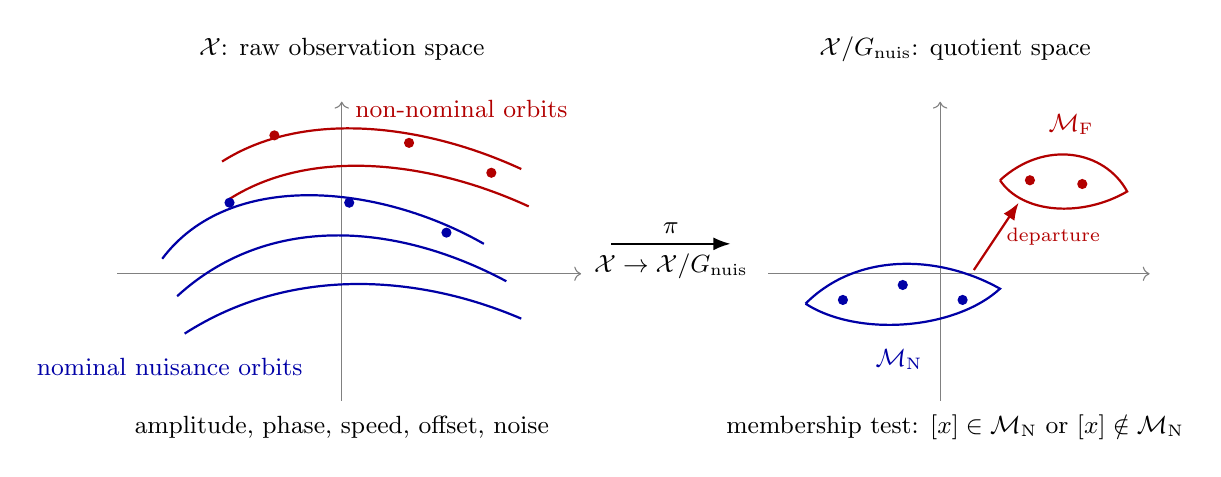
\begin{tikzpicture}[
    scale=0.95,
    every node/.style={font=\small},
    orbit/.style={thick},
    point/.style={circle, fill, inner sep=1.3pt},
    arrow/.style={-{Latex[length=2.2mm]}, thick},
    manifold/.style={thick}
]
% ---- left panel: raw observation space ----
\node at (0,3.0) {\(\X\): raw observation space};
\draw[->, gray] (-3,0) -- (3.2,0);
\draw[->, gray] (0,-1.7) -- (0,2.3);

\draw[orbit, blue!65!black] (-2.4,0.2) .. controls (-1.5,1.4) and (0.5,1.2) .. (1.9,0.4);
\draw[orbit, blue!65!black] (-2.2,-0.3) .. controls (-1.0,0.8) and (0.7,0.7) .. (2.2,-0.1);
\draw[orbit, blue!65!black] (-2.1,-0.8) .. controls (-0.7,0.1) and (1.0,0.0) .. (2.4,-0.6);
\draw[orbit, red!70!black] (-1.6,1.5) .. controls (-0.5,2.2) and (1.1,2.0) .. (2.4,1.4);
\draw[orbit, red!70!black] (-1.5,1.0) .. controls (-0.4,1.7) and (1.2,1.5) .. (2.5,0.9);

\node[point, blue!65!black] at (-1.5,0.95) {};
\node[point, blue!65!black] at (0.1,0.95) {};
\node[point, blue!65!black] at (1.4,0.55) {};
\node[point, red!70!black] at (-0.9,1.85) {};
\node[point, red!70!black] at (0.9,1.75) {};
\node[point, red!70!black] at (2.0,1.35) {};

\node[blue!65!black] at (-2.3,-1.25) {nominal nuisance orbits};
\node[red!70!black] at (1.6,2.2) {non-nominal orbits};
\node at (0,-2.05) {amplitude, phase, speed, offset, noise};

% ---- projection ----
\draw[arrow] (3.6,0.4) -- (5.2,0.4)
  node[midway, above] {\(\pi\)}
  node[midway, below] {\(\X \to \quotient\)};

% ---- right panel: quotient space ----
\node at (8.2,3.0) {\(\quotient\): quotient space};
\draw[->, gray] (5.7,0) -- (10.8,0);
\draw[->, gray] (8.0,-1.7) -- (8.0,2.3);

\draw[manifold, blue!65!black]
    (6.2,-0.4) .. controls (6.9,0.3) and (8.0,0.25) .. (8.8,-0.2)
    .. controls (8.2,-0.75) and (6.9,-0.85) .. (6.2,-0.4);
\node[blue!65!black] at (7.45,-1.15) {\(\Mnominal\)};

\draw[manifold, red!70!black]
    (8.8,1.25) .. controls (9.4,1.8) and (10.2,1.65) .. (10.5,1.1)
    .. controls (9.9,0.75) and (9.1,0.8) .. (8.8,1.25);
\node[red!70!black] at (9.75,2.0) {\(\Mfault\)};

\node[point, blue!65!black] at (6.7,-0.35) {};
\node[point, blue!65!black] at (7.5,-0.15) {};
\node[point, blue!65!black] at (8.3,-0.35) {};
\node[point, red!70!black] at (9.2,1.25) {};
\node[point, red!70!black] at (9.9,1.2) {};

\draw[arrow, red!70!black] (8.45,0.05) -- (9.05,0.95)
  node[midway, right] {\scriptsize departure};

\node[align=center] at (8.2,-2.05) {%
membership test: \([x]\in\Mnominal\) or \([x]\notin\Mnominal\)};
\end{tikzpicture}
\caption{Functional manifolds as quotient geometry. In raw observation space,
nuisance transformations generate extended orbits of observations that share
the same latent physical state. The quotient projection \(\pi\) collapses
those orbits into equivalence classes, exposing compact nominal and
non-nominal functional regions. Diagnosis is then a membership test in
\(\Mnominal\) rather than a partition of labelled observations.}
\label{fig:quotient_manifold_concept}
\end{figure}

This structural approach fundamentally clarifies the formal distinction between anomaly detection and discrete classification. A supervised classifier is optimized to learn an explicitly labeled partition of raw observations. In contrast, a quotient-space diagnostic operator optimizes a representation space wherein physically equivalent observations are mapped to identical topological classes. While categorical operational labels may subsequently be assigned to these bounded regions, the geometric regions structurally precede any semantic labeling; this exact procedure is detailed in Section~\ref{sec:emergent_classification}.

%---------------------------------------------------------------------
\subsection{The saturation radius}
\label{subsec:saturation_radius}
%---------------------------------------------------------------------

The companion report \citep{disanti2026inverse} proposes that a regime becomes
learnable when its geometric descriptors stabilize under additional
observations, written informally as
\begin{equation}
H(n)\to H^*,\qquad
r_{\max}(n)\to r^*,\qquad
V(n)\to V^*,
\label{eq:saturation_informal}
\end{equation}
for an entropy, a radius and a volume descriptor. As stated,
\eqref{eq:saturation_informal} is a description of observed behaviour rather
than a claim with a definite content: neither the estimators nor the mode of
convergence is specified. We therefore fix one descriptor precisely, the
radius, and show that doing so brings saturation within reach of the same
machinery used in Section~\ref{sec:computational_realization}.

Let \(\phi:\X\to\Z\) be a representation map and let \(\nu\) denote the law
induced on \(\Z\) by drawing \(\eta\) from the nominal nuisance law and
applying \(\phi\circ F(\theta_{\mathrm N},\cdot)\). Fix a reference point
\(c\in\Z\), for instance the mean of \(\nu\), and define the scalar
\begin{equation}
D = d\bigl(\phi(x),c\bigr), \qquad x = F(\theta_{\mathrm N},\eta),
\label{eq:radial_variable}
\end{equation}
with distribution function \(F_D\).

\begin{definition}[Population and empirical saturation radius]
\label{def:saturation_radius}
For \(p\in(0,1)\) the \emph{population \(p\)-radius} of the nominal regime is
the quantile
\begin{equation}
R_p = F_D^{-1}(p) = \inf\{r\ge 0 : F_D(r)\ge p\},
\label{eq:population_radius}
\end{equation}
and given \(n\) nominal observations with radial values
\(D_1,\ldots,D_n\) the \emph{empirical \(p\)-radius} \(\widehat R_p(n)\) is the
corresponding empirical quantile. The descriptor \(r_{\max}(n)\) of
\eqref{eq:saturation_informal} is the case \(p\to 1\), and the \(p_{95}\) and
\(p_{98}\) radii used in the companion work are the cases \(p=0.95\) and
\(p=0.98\).
\end{definition}

The primary utility of Definition~\ref{def:saturation_radius} is establishing that the specific object being estimated rigorously exists and is strictly finite; this property does not derive inherently from the informal statement \eqref{eq:saturation_informal}, but rather follows as a direct consequence of the structural properties established in Section~\ref{sec:quotient_formulation}.

\begin{corollary}[Finiteness of the saturation radius]
\label{cor:finite_radius}
Under Assumption~\ref{ass:compact_eta}, if \(\phi\) is continuous then \(D\) is
a bounded random variable and \(R_p<\infty\) for every \(p\in(0,1)\); moreover
\(\sup_{\eta\in\EtaSpace} D<\infty\), so the regime has a finite radius in the
Hausdorff sense.
\end{corollary}

\begin{proof}
By Proposition~\ref{prop:compactness} the closure
\(\overline{\mathcal{O}_{\mathrm N}}\) is compact, and \(\phi\) is continuous,
so \(\phi(\overline{\mathcal{O}_{\mathrm N}})\) is compact in \(\Z\). The map
\(z\mapsto d(z,c)\) is continuous, and a continuous real function on a compact
set is bounded and attains its supremum. Hence \(D\) is bounded and every
quantile of \(F_D\) is finite.
\end{proof}

Corollary~\ref{cor:finite_radius} is the precise sense in which the compactness
result of Section~\ref{sec:quotient_formulation} underwrites the
finite-Hausdorff-radius premise of the functional-topological foundation
discussed in Remark~\ref{rem:blueprints_relation}. Saturation can then be
stated as a convergence claim about an estimator of a finite quantity.

\begin{proposition}[Consistency of the empirical saturation radius]
\label{prop:radius_consistency}
Let \(D_1,D_2,\ldots\) be independent draws of \eqref{eq:radial_variable} and
suppose \(F_D\) is strictly increasing in a neighbourhood of \(R_p\), so that
the quantile is unique. Then
\begin{equation}
\widehat R_p(n) \longrightarrow R_p \qquad \text{almost surely as } n\to\infty .
\label{eq:radius_consistency}
\end{equation}
\end{proposition}

\begin{proof}
By the Glivenko--Cantelli theorem the empirical distribution function
converges to \(F_D\) uniformly and almost surely. Uniqueness of the quantile at
level \(p\) transfers uniform convergence of the distribution function to
pointwise convergence of the quantile function at \(p\); see, for example,
\citet[Sec.~2.3]{serfling1980} or \citet[Lemma~21.2]{vandervaart1998}.
\end{proof}

Proposition~\ref{prop:radius_consistency} makes
\eqref{eq:saturation_informal} a theorem rather than an observation, and it
identifies the limit as a specific population quantile. It is, however, purely
asymptotic, and therefore silent on the question the operational criterion
actually poses, namely how many observations suffice.

%---------------------------------------------------------------------
\subsection{Finite-sample certification of saturation}
\label{subsec:saturation_certification}
%---------------------------------------------------------------------

The requisite finite-sample guarantees are supplied by the statistical argument developed in Section~\ref{subsec:distribution_free}. Definition~\ref{def:saturation_radius} explicitly formulates the saturation radius as a quantile of a nominal distribution estimated from a finite sample set. This constitutes precisely the identical estimation problem as the local operational radius, differing solely in the underlying domain: distances within the representation space \(\Z\) as opposed to scalar residuals in \(\R\). Because Proposition~\ref{prop:coverage} is formulated for an arbitrary exchangeable scalar sequence, it applies unaltered to the radial variables.

This forward dependency is noted explicitly for clarity. Proposition~\ref{prop:coverage} is established in Section~\ref{subsec:distribution_free} rather than in the present section because its primary operational function concerns the calibration of the terminal decision boundary. However, it constitutes a fundamental result regarding exchangeable real-valued sequences and remains logically independent of any properties specific to diagnostic residuals, as formalized in Remark~\ref{rem:saturation_link}. Consequently, the subsequent corollary invokes this later proposition without introducing logical circularity.

\begin{corollary}[Distribution-free certification of the saturation radius]
\label{cor:saturation_certification}
Let \(D_1,\ldots,D_n,D_{n+1}\) be exchangeable with an atomless marginal, let
\(\alpha=1-p\), and set
\begin{equation}
\widehat R^{\,\star}_p = D_{(k_\alpha)},
\qquad k_\alpha = \bigl\lceil p\,(n+1) \bigr\rceil .
\label{eq:radius_order_statistic}
\end{equation}
Then, provided \(n\ge 1/\alpha-1\),
\begin{equation}
p \;\le\; \Prob\bigl(D_{n+1}\le \widehat R^{\,\star}_p\bigr)
  \;=\; \frac{k_\alpha}{n+1}
  \;\le\; p+\frac{1}{n+1},
\label{eq:radius_coverage}
\end{equation}
and \(\widehat R^{\,\star}_p\) equals the largest observed radial value
\(D_{(n)}\) precisely when \(1/\alpha-1\le n<2/\alpha-1\).
\end{corollary}

\begin{proof}
Apply Proposition~\ref{prop:coverage}, Corollary~\ref{cor:min_commissioning}
and Corollary~\ref{cor:degenerate_range} with \(\residual_i\) replaced by
\(D_i\). Neither the coverage argument nor the two corollaries uses any
property of the scalar sequence beyond exchangeability and atomlessness.
\end{proof}

Corollary~\ref{cor:saturation_certification} analytically unifies the functional-topological and statistical halves of the framework. Practically, certifying that a regime's empirical extent correctly covers a population fraction \(p\) of its nominal orbit strictly requires at least \(1/\alpha-1\) independent observations (yielding \(n=49\) at \(p=0.98\)). Moreover, because the certified topological radius is identically the sample maximum throughout the interval \(1/\alpha-1\le n<2/\alpha-1\), any empirical saturation curve that appears to stabilize within this band has merely stabilized at the most highly variable order statistic available. This apparent stabilization is an artifact of the finite-sample estimator rather than physical evidence of true regime saturation. Consequently, for \(p=0.98\), securing a non-degenerate saturation radius demands \(n\ge 99\).

\begin{remark}[Plug-in reference points and exchangeability]
\label{rem:plugin_centroid}
The theoretical radial variable \eqref{eq:radial_variable} is formalized against a strictly fixed reference point \(c\). In operational practice, \(c\) is typically estimated directly from acquired data; additionally, prior implementations estimate the specific projection space utilized for distance measurement from this identical sample set. Both data-dependent substitutions induce strict statistical dependence among the scalar variables \(D_1,\ldots,D_n\), consequently violating the fundamental exchangeability of the augmented sequence. Under these conditions, Corollary~\ref{cor:saturation_certification} holds only asymptotically, exhibiting a finite-sample error that decays as the reference parameters converge. The rigorous structural remedy is the split-sample strategy utilized in Remark~\ref{rem:optional_stopping}: one must compute the reference centroid (and the projection subspace) over a block of nominal observations strictly disjoint from the block utilized to evaluate the empirical saturation radius. This formally restores sequence exchangeability by construction, trading sample efficiency for analytical exactness.
\end{remark}

\begin{remark}[Interpretive limits of the saturation curve]
\label{rem:saturation_semantics}
The empirical flattening of the statistic \(\widehat R_p(n)\) constitutes an operational stopping heuristic, not a formal mathematical proof that the population parameter \(R_p\) has been perfectly recovered. This mirrors the logic establishing that empirical convergence of the commissioning criterion fails to guarantee exact recovery of the underlying population residual quantile (see Remark~\ref{rem:stopping_semantics}). Specifically, an upper quantile estimated from limited extreme-tail samples may exhibit extended periods of zero variance, only to shift discontinuously upon the arrival of a rare nominal extremum. Corollary~\ref{cor:saturation_certification} is entirely consistent with this phenomenon: it strictly bounds probabilistic coverage at a fixed sample size \(n\), but provides no constraint on the sequential increments of the trajectory. Accordingly, claims regarding geometric stabilization at specific sample sizes must be interpreted strictly as descriptions of an observed empirical trajectory, whereas the rigorous coverage statement constitutes the sole statistically guaranteed proposition.
\end{remark}

\begin{remark}[Tension between convergence heuristics and exact certification]
\label{rem:saturation_tension}
The quantitative evaluations documented in Section~\ref{sec:results} elevate the theoretical caveat of Remark~\ref{rem:saturation_semantics} into a consequential operational constraint. Within the degenerate sample range, the certified empirical radius explicitly equals the absolute sample maximum; thus, its expectation systematically drifts upward as \(n\) increases. In controlled simulations mapping nominal data at \(p=0.98\), the expected estimate diverges from approximately \(2\%\) above the population value \(R_p\) at \(n=49\) to roughly \(6\%\) above at \(n=98\). It then drops discontinuously at \(n=99\), the precise threshold where the first interior order statistic becomes mathematically accessible. Therefore, a saturation curve utilizing the formally certified estimator mathematically \emph{cannot} exhibit true stabilization within this degenerate band; any apparent plateau constitutes an artifact of evaluating the sequential maximum over a growing sample.

Conversely, standard interpolated quantile estimators exhibit precisely the complementary failure mode. While they generate smoothly convergent curves approaching \(R_p\) monotonically from below, they consistently undercover the target probability across all evaluated finite-sample regimes. Consequently, appealing visual convergence and rigorous statistical coverage exist in strict methodological tension: the interpolated estimator responsible for a smooth, seemingly convergent saturation plot inherently fails the exact certification requirement, while the rigorously certifiable estimator actively precludes visual plateauing until the degenerate sample regime is strictly surpassed. Operational saturation reporting must therefore couple the trajectory plot with an explicit statement of attained statistical coverage, strictly requiring \(n\ge 2/\alpha-1\).
\end{remark}

\begin{remark}[The saturation radius serves as a geometric diagnostic, not a classifier]
\label{rem:radius_not_detector}
A critical empirical constraint restricts the analytical scope of saturation analysis. When evaluating the formally certified radius for distinct simulated regimes utilizing a shared, two-dimensional nominal projection, the resulting separation is negligible: observed ratios of fault-to-nominal radii strictly remain within \(0.98\) to \(1.04\). The fundamental cause is physical mechanics. A principal component projection truncating a raw vibration signal is overwhelmingly dominated by high-energy primary shaft harmonics. In contrast, early-stage fault signatures typically manifest as low-amplitude impulse trains orthogonal to the primary axes, contributing negligible variance to the leading eigen-directions. Conversely, utilizing the exact same physical simulator, nominal-only calibration data, and statistical decision rule yields a \(99\)--\(100\%\) detection rate when manifold membership is evaluated via the orthogonal reconstruction residual (see Section~\ref{sec:results}).

Two structural consequences emerge. First, a geometric saturation plot constitutes empirical evidence strictly regarding the adequacy of nominal geometry sampling; it provides zero theoretical guarantee regarding regime separability and must not be invoked as proof of diagnostic efficacy. Second, this physical masking mechanism provides the formal justification for architecting the diagnostic framework around orthogonal residuals---as formulated in Section~\ref{sec:computational_realization}---rather than topological radii within a low-dimensional projection. Specifically, Assumption~\ref{ass:residual_proxy} requires the scalar anomaly score to accurately track distance to the nominal manifold, a geometric requirement that a leading-variance radius demonstrably fails to satisfy.
\end{remark}

% ============================================================================
\section{Emergent Classification via Expert Feedback}
\label{sec:emergent_classification}
% [MERGE: COMPANION "Emergent Classification Through Expert Feedback" and
% "Consequences for Classification"] + [NEW: per-class coverage corollary,
% set-valued formulation, and an explicit separation-versus-coverage scope
% statement grounded in the Experiment 6 negative result]. WRITTEN.

Sections~\ref{sec:quotient_formulation}--\ref{sec:manifolds_saturation} analytically formulate the topological properties of a single operational state: the nominal regime. The present section extends this geometric construction to regimes incorporating multiple recovered operational states, establishing the formal interface between anomaly detection and fault classification. The resulting theoretical structure is fundamentally asymmetric: the quotient geometry yields rigorous, distribution-free guarantees regarding when a specific operational class should \emph{not} be rejected, while offering minimal analytical traction regarding the exclusion of competing classes. This structural asymmetry constitutes the primary focus of the section.

%---------------------------------------------------------------------
\subsection{Two levels of classification}
\label{subsec:two_levels}
%---------------------------------------------------------------------

Classification within this geometric framework operates across two distinct hierarchical levels; conflating these levels frequently obfuscates the analytical advantages provided by the inverse-problem perspective.

The primary level is \emph{structural} classification. An acquired observation is geometrically assigned to a formally recovered functional region, to an emergent sub-manifold that has not yet achieved topological saturation, to a transition trajectory between regions, or to the complement of all known regions (the null set). This topological assignment operates entirely independently of semantic labels: it is strictly induced by the geometric structure of the quotient space and the rigorously calibrated membership rule \eqref{eq:membership}.

The secondary level is \emph{operational} classification. Once an empirical region has achieved rigorous topological stabilization as defined in Section~\ref{sec:manifolds_saturation}, a domain expert or downstream control policy may superimpose semantic meaning onto the geometry: e.g., nominal operation, permissible variation, friction-induced thermal degradation, or a specific mechanical fault regime. Consequently, classification capability is not conditionally dependent upon a priori label availability; it manifests initially as strict geometric membership and only subsequently acquires semantic interpretation.

%---------------------------------------------------------------------
\subsection{Manifold-level labelling}
\label{subsec:manifold_labelling}
%---------------------------------------------------------------------

Let \(\{\mathcal{M}_j\}_{j=1}^{k}\) denote a family of recovered compact
regions in \(\quotient\), of which \(\Mnominal\) is one. Labels are attached
at the level of regions rather than of samples, through a map
\begin{equation}
L:\{\mathcal{M}_j\}_{j=1}^{k}\longrightarrow \mathcal{Y},
\qquad L(\mathcal{M}_j)=y_j .
\label{eq:labelling_map}
\end{equation}
The critical methodological departure from standard supervised practice lies in the fundamental object subjected to labeling. Whereas a traditional supervised classifier necessitates high-volume point-wise annotations \(x_i\mapsto y_i\) distributed across individual samples, the geometric framework requires the domain expert to supply the manifold-level mapping \(\mathcal{M}_j\mapsto y_j\) exactly once per recovered topological region. Consequently, the requisite labeling effort scales strictly with the intrinsic number of operational regimes rather than the volume of acquired observations.

Given a residual \(\residual_j\) for each region, in the sense of
Assumption~\ref{ass:residual_proxy}, and a radius \(\tau_j\) calibrated for
that region by Proposition~\ref{prop:coverage}, the admissible set for an
observation is
\begin{equation}
\Gamma(x) \;=\; \bigl\{\, j \in \{1,\ldots,k\} \;:\; \residual_j(x)\le\tau_j \,\bigr\},
\label{eq:admissible_set}
\end{equation}
and the reported diagnosis is
\begin{equation}
\hat y(x)=
\begin{cases}
L(\mathcal{M}_j), & \Gamma(x)=\{j\},\\[2pt]
\{L(\mathcal{M}_j)\}_{j\in\Gamma(x)}, & |\Gamma(x)|>1 \quad\text{(ambiguous)},\\[2pt]
\mathrm{unknown}, & \Gamma(x)=\emptyset .
\end{cases}
\label{eq:set_valued_rule}
\end{equation}

Formulating the decision rule \eqref{eq:set_valued_rule} as a set-valued output rather than a point-wise \(\arg\min\) operator is a structural necessity rather than a stylistic convention. It accurately reflects the rigorous statistical calibration established in Section~\ref{sec:computational_realization} and renders the two primary diagnostic failure modes analytically explicit, rather than obfuscating them beneath a heuristic nearest-region assignment. Specifically, an anomalous observation may satisfy the inclusion criteria for no established region (constituting the formal diagnostic abstention anticipated by \eqref{eq:membership}), or it may simultaneously satisfy the criteria for multiple overlapping regions (ambiguity). Methodologically, this formulation constitutes the class-conditional (or Mondrian) architecture of a conformal predictor \citep{vovk2005,shafer2008}; crucially, it is derived constructively from the quotient manifold geometry rather than being imposed as an external statistical assumption.

\begin{corollary}[Per-class non-rejection]
\label{cor:per_class_coverage}
Fix a region \(\mathcal{M}_j\) and suppose the residuals
\(\residual_j\) evaluated on observations from regime \(j\) satisfy
Assumption~\ref{ass:exchangeability}, with \(\tau_j\) calibrated from
\(n_j\ge 1/\alpha_j-1\) such observations by
\eqref{eq:radius_order_statistic}. Then for a further observation \(x\) drawn
from regime \(j\),
\begin{equation}
\Prob\bigl(j\in\Gamma(x)\bigr)\;\ge\;1-\alpha_j .
\label{eq:per_class_coverage}
\end{equation}
Consequently the true regime is retained in the admissible set with
probability at least \(1-\alpha_j\), simultaneously for every regime, without
any assumption on the residual distributions and without any calibration data
from competing regimes.
\end{corollary}

\begin{proof}
Apply Proposition~\ref{prop:coverage} to the exchangeable sequence generated
by \(\residual_j\) on regime \(j\); the event \(\{j\in\Gamma(x)\}\) is
precisely \(\{\residual_j(x)\le\tau_j\}\). The statement is per-regime and the
regimes are calibrated independently, so no joint assumption is required.
\end{proof}

Corollary~\ref{cor:per_class_coverage} formalizes the primary theoretical advantage of this framework. Because each manifold region is calibrated exclusively against its own nominal behavior, a novel regime can be incorporated post-deployment without necessitating the recalibration of pre-existing regions. A regime for which empirical data is entirely absent simply contributes a null set to the admissible region \(\Gamma(x)\). This rigorously defines the mechanism by which the classification taxonomy may structurally expand: appending a new region \(\mathcal{M}_{k+1}\) alters the admissible set \eqref{eq:admissible_set} by precisely one additive term, leaving the non-rejection guarantee \eqref{eq:per_class_coverage} strictly invariant for all pre-existing classes \(j\le k\).

This geometric formulation entails several structural consequences originally anticipated in the companion report \citep{disanti2026inverse}: distinct topological regions may map to an identical semantic label if they constitute disjoint operational variants of a single regime; conversely, a singular nominal label may mathematically resolve into multiple distinct geometric regions if the underlying operational behavior exhibits structural heterogeneity. Furthermore, an anomalous observation is not algorithmically forced into the nearest calibrated class, and diagnostic expert effort is systematically allocated to verifying bounded topological regions rather than labeling individual point samples.

%---------------------------------------------------------------------
\subsection{What coverage does not give: separation}
\label{subsec:coverage_not_separation}
%---------------------------------------------------------------------

Corollary~\ref{cor:per_class_coverage} exclusively bounds the probability of erroneously \emph{excluding} the true generating regime. It provides zero theoretical guarantee against erroneously \emph{including} a competing regime; this analytical distinction represents a fundamental limitation rather than a minor technicality.

\begin{remark}[Statistical coverage does not imply geometric discrimination]
\label{rem:coverage_not_discrimination}
The mathematical inequality \eqref{eq:per_class_coverage} does not theoretically bound the cardinality \(|\Gamma(x)|\). The constituent acceptance regions \(\{\residual_j\le\tau_j\}\) are calibrated entirely independently and may exhibit arbitrary geometric overlap. In the degenerate limit, if two distinct regions remain geometrically indistinguishable under the specified residual operators, every observation originating from either regime will be mutually admitted by both boundaries, yet the formal coverage guarantee \eqref{eq:per_class_coverage} remains perfectly valid. Consequently, a rigorous statistical guarantee regarding non-rejection is entirely compatible with a terminal diagnosis that is persistently ambiguous. Actively minimizing \(|\Gamma(x)|\) necessitates establishing strict geometric \emph{separation} between regions; this is fundamentally a property of the learned representation rather than the statistical calibration, and it does not derive analytically from the quotient formulation (Section~\ref{sec:quotient_formulation}), topological compactness, or any order-statistic argument.
\end{remark}

\begin{remark}[Structural obstructions to classification]
\label{rem:classification_obstructions}
The specific computational architecture detailed in Section~\ref{sec:computational_realization} inherently fails to provide this geometric separation due to two distinct structural limitations, both of which are empirically validated in Section~\ref{sec:results}.

First, a scalar residual constitutes a strictly non-injective (many-to-one) mapping. The diagnostic rule \eqref{eq:decision_rule} quantifies the magnitude of departure from the nominal region via a singular scalar value; the multidimensional \emph{direction} of that departure is fundamentally irrevocably lost. Consequently, anomaly detection and fault classification constitute mathematically distinct problems within this framework. Specifically, classifying among \(k\) fault types necessitates \(k\) distinct residual operators, each possessing its own independent representation space and local calibration, rather than applying \(k\) discrete thresholds to a single global residual.

Second, as previously established, the low-dimensional radial diagnostic defined in Section~\ref{sec:manifolds_saturation} mathematically fails to separate the operational regimes it characterizes. Empirical evaluation on simulated data within a shared two-dimensional nominal projection yields fault-to-nominal radius ratios constrained between \(0.98\) and \(1.04\) (Section~\ref{sec:results})---indicating zero effective separability---despite the identical simulation exhibiting \(99\)--\(100\%\) anomaly detection efficacy via the orthogonal reconstruction residual. Topological saturation of a geometric region and its geometric separability from adjacent regions constitute strictly independent mathematical properties; empirical evidence validating the former provides no theoretical support for the latter.
\end{remark}

This structural limitation strictly delineates the scope of fault classification within the present framework, mathematically formalizing the analytical gap identified in the companion technical note \citep{disanti2026quotient} without purporting to resolve it. The established theoretical results prove that diagnosis necessarily factors through the defined quotient space (Proposition~\ref{prop:quotient_diagnosis})---ensuring that a structurally correct classifier theoretically exists as a function of the equivalence class \([x]\) alone. It further proves that geometric regions, once extracted, can be semantically labeled and calibrated independently with exact, distribution-free per-class validity (Corollary~\ref{cor:per_class_coverage}), while rigorously preserving both diagnostic abstention and ambiguity \eqref{eq:set_valued_rule}. However, the present formulation does not prove that any specific empirical representation guarantees separability among non-nominal fault regions. Section~\ref{sec:future_work} outlines the specific experimental validation required to evaluate such separation.

% ============================================================================
\section{Computational Realization and Local Calibration}
\label{sec:computational_realization}
% [MERGE: TECHNOTE Sec.6 + TRB Sec.3 Method] + [NEW: Prop. 3, Cor. 3,
% Remarks 5-9]. WRITTEN.

Sections~\ref{sec:observation_model}--\ref{sec:emergent_classification} mathematically characterize the diagnostic object: a compact, connected nominal region \(\Mnominal\) residing within a quotient topological space, where an anomaly is formally defined as the failure of set membership. However, this theoretical characterization does not inherently constitute an executable algorithm. Specifically, two computational quantities must be defined before the theoretical membership test \eqref{eq:membership} can be evaluated on empirical data: a computable surrogate for the abstract distance to \(\Mnominal\), and a strictly calibrated decision boundary defined upon that surrogate.

This section operationalizes both requirements. Section~\ref{subsec:representation_operator} defines the representation operator and formalizes the reconstruction residual as the computable distance surrogate. Section~\ref{subsec:scale_transfer} demonstrates that, as a direct consequence of Proposition~\ref{prop:quotient_diagnosis}, the functional representation exhibits structural transferability across physical assets, whereas the numerical scale of the residual strictly does not; this fundamental asymmetry dictates that a singular global decision boundary is analytically invalid. Finally, Sections~\ref{subsec:mc_calibration} and \ref{subsec:distribution_free} derive the local calibration procedure and its exact finite-sample guarantees. Specifically, the central novel result (Proposition~\ref{prop:coverage}) establishes that an operational radius formulated as a specific order statistic of nominal commissioning residuals achieves exact prescribed coverage entirely independent of the underlying residual distribution, while Corollary~\ref{cor:min_commissioning} explicitly translates this statistical bound into a deterministic minimum commissioning duration.

Throughout this section we index physical assets, or more generally
independently commissioned monitoring environments, by \(k\).

%---------------------------------------------------------------------
\subsection{Representation operator and diagnostic residual}
\label{subsec:representation_operator}
%---------------------------------------------------------------------

Let \(E:\X\rightarrow\Z\) be an encoder and \(D:\Z\rightarrow\X\) a
decoder, with reconstruction
\begin{equation}
\hat{x} = D(E(x)),
\label{eq:reconstruction}
\end{equation}
and define the \emph{diagnostic residual}
\begin{equation}
\residual(x) = \frac{1}{n_w}\bigl\|x-\hat{x}\bigr\|_2^2 .
\label{eq:residual}
\end{equation}
In the present realization \(E\) and \(D\) are the encoder and decoder of a
one-dimensional convolutional autoencoder trained exclusively on nominal
windows generated by Monte Carlo sampling of \(\EtaSpace\); autoencoders
have long been used both as nonlinear representation learners
\citep{hinton2006} and as reconstruction-based anomaly detectors
\citep{sakurada2014}. No non-nominal observation is used at any stage of
representation learning.

\begin{assumption}[Residual--distance proxy]
\label{ass:residual_proxy}
The diagnostic residual \(\residual(x)\) is treated as a computable proxy
that is monotonically related to distance to the nominal set:
\begin{equation}
\residual(x) \;\approx\; d\bigl(x,\mathcal{O}_{\mathrm N}\bigr).
\label{eq:distance_proxy}
\end{equation}
\end{assumption}

\begin{remark}[Ambient distance evaluation and metric constraints]
\label{rem:distance_lives_in_X}
The distance invoked in \eqref{eq:distance_proxy} constitutes the ambient Euclidean metric native to the observation space \(\X\), not a rigorously defined metric on the quotient space \(\quotient\); this formulation is a deliberate structural choice rather than an analytical simplification.

The space \(\quotient\) is equipped exclusively with the quotient topology; it does not inherently carry a metric, and the most natural candidate pseudometric is mathematically degenerate in this context. Specifically, the standard quotient pseudometric \(\inf_{g,h\in\Gnuis}\lVert g\cdot x - h\cdot y\rVert\) induced by the group defined in Section~\ref{sec:quotient_formulation} trivially vanishes for every arbitrary pair of non-zero observation windows, because the unbounded scalar multiplicative actions of \(\Gnuis\) can asymptotically drive both arguments toward the origin. Consequently, a non-degenerate quotient distance necessarily requires restricting the group action---a theoretical construction outlined in Remark~\ref{rem:quotient_radius} but deliberately not implemented in the present computational realization.

This limitation restricts the analytical claims supported by the quotient formulation. Crucially, the ambient Euclidean distance in \(\X\) is strictly \emph{not} nuisance-invariant: two mathematically nuisance-equivalent observation windows differing exclusively by a scalar gain parameter inherently lie at a strictly non-zero ambient distance. Therefore, any observed near-invariance of the diagnostic residual \(\residual\) across nuisance fluctuations constitutes an \emph{empirical property of the optimized operator}, not an analytical consequence of the quotient geometry. The quotient formulation rigorously defines the theoretical problem---specifying the topological object requiring recovery, proving that non-injectivity constitutes underlying structure rather than stochastic noise, and formalizing the diagnostic decision as a set membership test rather than an arbitrary threshold on a scalar index---whereas every numerical quantity evaluated in this framework is strictly computed within the ambient space \(\X\).

This geometric limitation is explicitly verified by empirical measurement. As detailed in Section~\ref{subsec:disc_scale}, the absolute residual scale diverges across equivalent assets by a factor approaching three; furthermore, Section~\ref{subsec:results_nasa} demonstrates that a local operational radius normalized by the specific asset's median residual exhibits order-of-magnitude greater stability across random initialization seeds compared to the unnormalized radius. Both empirical results confirm that while the observed invariance is highly functional, it remains strictly partial and must be attributed entirely to the capacity of the learned representation operator rather than to the underlying topological geometry.
\end{remark}

Assumption~\ref{ass:residual_proxy} functions as a strictly operational hypothesis; it is not an analytical consequence of the optimization objective. Minimizing mean-squared reconstruction error over nominal data provides no formal mathematical guarantee that the resulting residual \(\residual\) will be isometric, or even monotonic, with respect to any rigorously defined metric upon \(\quotient\). Consequently, the validity of this assumption must be established empirically. This empirical evaluation is documented in Section~\ref{sec:results}, utilizing the distributional separation between nominal and non-nominal residuals as the primary evidentiary basis. The lack of a formal guarantee is explicitly documented as a structural limitation in Section~\ref{sec:limitations}.

The fundamental theoretical claim of this framework does not assert that mean-squared reconstruction error constitutes the optimal or unique residual operator. Rather, it establishes that a suitably formulated scalar residual can effectively function as an operational test for set membership within the nominal quotient manifold. Any scalar score satisfying the qualitative monotonic requirement of \eqref{eq:distance_proxy} may be seamlessly substituted; viable alternatives include latent probabilistic likelihoods, Mahalanobis distances within the representation space \(\Z\), energy-based scores, diffusion or denoising criteria, autoregressive predictive errors, or explicitly physics-informed residuals. Crucially, the local statistical calibration theory developed in Section~\ref{subsec:distribution_free} is formulated for an entirely arbitrary continuous residual sequence, rendering the analytical guarantees strictly invariant to the specific choice of representation operator.

%---------------------------------------------------------------------
\subsection{Why the representation transfers but its scale does not}
\label{subsec:scale_transfer}
%---------------------------------------------------------------------

Proposition~\ref{prop:quotient_diagnosis} states that the ideal diagnostic
map factors through the quotient. Write that ideal map as the membership
predicate
\begin{equation}
h(x) = \indicator\bigl[\,[x]\notin\Mnominal\,\bigr],
\label{eq:ideal_predicate}
\end{equation}
so that \(h=\bar h\circ\pi\) by Proposition~\ref{prop:quotient_diagnosis},
and \(h\) is constant on nuisance orbits. The computable surrogate actually
evaluated on data is
\begin{equation}
h_\tau(x) = \indicator\bigl[\,\residual(x) > \tau\,\bigr].
\label{eq:surrogate_predicate}
\end{equation}

\begin{remark}[Asymmetric inheritance of nuisance invariance]
\label{rem:scale_not_invariant}
The computable surrogate \eqref{eq:surrogate_predicate} strictly fails to inherit the theoretical orbit-invariance of the ideal predicate \eqref{eq:ideal_predicate}. The scalar residual \(\residual\) operates fundamentally as a function upon the ambient space \(\X\), not the quotient \(\quotient\). It is analytically not \(\Gnuis\)-invariant, because the absolute reconstruction error generated by any fixed operator pair \((E,D)\) intrinsically fluctuates along a given nuisance orbit, even when the underlying operational latent state remains static. Consequently, for any globally fixed threshold \(\tau\), the defined level set \(\{\residual = \tau\}\) cannot constitute the exact \(\pi\)-preimage of a bounded subset of the quotient space, and the surrogate decision function \(h_\tau\) is provably not constant across orbits. The theoretical contribution of the quotient structure, established via Proposition~\ref{prop:quotient_diagnosis}, guarantees exclusively that a structurally \emph{correct} diagnostic decision theoretically exists as a function of the equivalence class \([x]\) alone. Translating this guarantee to the ambient residual \(\residual\) mandates calibrating the threshold \(\tau\) such that the resulting ambient level set accurately approximates the geometric boundary \(\partial\Mnominal\) specifically under the highly localized nuisance distribution physically realized by the specific asset under observation.
\end{remark}

Remark~\ref{rem:scale_not_invariant} induces a critical architectural constraint, mathematically dictating that statistical calibration must be executed per-asset rather than globally. The learned operator \((E,D)\) structurally encodes the geometric distinction between permissible nuisance variation and critical diagnostic divergence; this topological structure is a fundamental property of the asset family and is consequently fully transferable. However, the exact numerical magnitude of \(\residual\) is additionally confounded by highly localized parameters, including specific sensor coupling coefficients, mechanical mounting variances, idiosyncratic operating baselines, localized preprocessing artifacts, and the stochastic optimization trajectory that originally parameterized \((E,D)\); none of these scalar properties are analytically transferable. Consequently, the framework enforces a strict methodological separation:

\begin{itemize}[leftmargin=1.5em]
\item A singular representation operator \((E,D)\) is trained exactly once utilizing simulated nominal observations, and is subsequently held strictly fixed across all deployments;
\item A distinct scalar \emph{local operational radius} \(\tau_k^\star\) is independently calibrated for each monitored asset \(k\), estimated exclusively from that specific asset's localized nominal observations.
\end{itemize}

The decision rule for asset \(k\) at time \(t\) is then
\begin{equation}
\hat y\bigl(x_{k,t}\bigr) =
\begin{cases}
\text{anomalous}, & \residual(x_{k,t}) > \tau_k^\star,\\[2pt]
\text{nominal},   & \residual(x_{k,t}) \le \tau_k^\star .
\end{cases}
\label{eq:decision_rule}
\end{equation}

This prediction is falsifiable and is tested directly in
Section~\ref{sec:results}: transferring the residual \emph{scale} across
the simulation-to-field boundary should fail, while transferring the
representation and re-estimating only \(\tau_k^\star\) should not.

%---------------------------------------------------------------------
\subsection{Monte Carlo reference calibration}
\label{subsec:mc_calibration}
%---------------------------------------------------------------------

A reference boundary can be computed entirely in simulation. Let
\(\mu_{\mathrm{MC}}\) and \(\sigma_{\mathrm{MC}}\) denote the mean and
standard deviation of \(\residual\) over held-out nominal Monte Carlo
windows, and let \(q\in(0,1)\) denote a target nominal coverage level. A
parametric reference is
\begin{equation}
\taumc(q) = \mu_{\mathrm{MC}} + z_q\,\sigma_{\mathrm{MC}},
\label{eq:tau_mc_quantile}
\end{equation}
with \(z_q\) the corresponding standard-normal quantile; alternatively
\(\taumc(q)\) may be taken as the empirical \(q\)-quantile of the synthetic
nominal residual distribution.

The level \(q\) is not part of the mathematical formulation. It is an
operational risk parameter: lower values increase sensitivity at the cost of
false alarms, higher values reduce false alarms at the cost of delayed
detection of weak or incipient deviations.

\begin{remark}[\(\taumc\) is a reference, not a deployable radius]
\label{rem:mc_not_deployable}
By Remark~\ref{rem:scale_not_invariant}, \(\taumc(q)\) calibrates the
residual scale of the \emph{simulator}, not of any physical asset. It is
reported here because it is the natural baseline and because its failure is
informative, not because it is proposed as an operating point. The
corresponding experiment is the direct-transfer condition of
Section~\ref{sec:results}.
\end{remark}

%---------------------------------------------------------------------
\subsection{Distribution-free calibration of the local operational radius}
\label{subsec:distribution_free}
%---------------------------------------------------------------------

We now give the calibration procedure a guarantee. Before doing so it is
worth being explicit about what is being estimated, because the scalar form
of \(\tau_k^\star\) invites a misreading.

\begin{remark}[A set is being estimated, not a threshold tuned]
\label{rem:support_estimation}
The decision rule \eqref{eq:decision_rule} compares a scalar to a scalar, but
the object it defines is the region
\begin{equation}
\widehat{S}_k \;=\; \bigl\{\, x\in\X \;:\; \residual(x)\le\tau_k^\star \,\bigr\},
\label{eq:acceptance_region}
\end{equation}
a level set of the residual, and the guarantee below is a statement about the
nominal probability mass that \(\widehat{S}_k\) contains. The task is
therefore \emph{support estimation} rather than threshold calibration: no
trade-off between error types is being tuned, and no fault data is consulted
to place the boundary. This is the problem posed by
\citet{devroye1980}, who introduced support estimation precisely in order to
decide whether a new measurement belongs to the support of a distribution
observed so far, and it is the problem the one-class formulation of
\citet{scholkopf2001} and the minimum-volume-set literature
\citep{scott2006} address with different estimators.

The distinction matters for how the framework should be judged. A tuned
threshold is answerable to the error rates it achieves on labelled faults; an
estimated region with prescribed nominal coverage is answerable to whether it
attains that coverage, which can be checked without any fault observation
whatsoever. The residual supplies the family of candidate regions, indexed by
\(\tau\); Section~\ref{sec:quotient_formulation} supplies the reason a
bounded region exists to be estimated
(Corollary~\ref{cor:bounded_manifold}) and the reason the boundary of an
invariant set is a well-defined object in the quotient
(Proposition~\ref{prop:boundary_invariant}, with the scope recorded in
Remark~\ref{rem:orbit_not_invariant}); and the argument below selects a
member of the family with a distribution-free coverage property.
\end{remark}

\begin{remark}[Geometric constraints of level-set estimation]
\label{rem:level_not_shape}
The preceding analysis establishes a strict limitation regarding the estimated topological boundary. The described calibration procedure mathematically selects a single member from the one-parameter family of level sets \(\{\,\residual\le\tau\,\}_{\tau>0}\); crucially, the underlying geometric \emph{shape} of that acceptance region is deterministically governed by the functional form of \(\residual\) and remains entirely unestimated. Distinct residual operators inherently induce divergent topologies for identically distributed nominal data: linear subspace reconstruction errors generate regions elongated along retained principal axes; Mahalanobis distances yield multivariate ellipsoids; nearest-neighbor statistics produce unions of local Euclidean balls \citep{devroye1980}; and non-linear representations, such as one-class kernel methods \citep{scholkopf2001} or deep autoencoders, define complex manifolds devoid of closed-form topological descriptions. Proposition~\ref{prop:coverage} is theoretically indifferent to these geometric distinctions: each construction rigorously attains the prescribed statistical coverage, yet coverage probability alone is analytically incapable of distinguishing a highly conformal region from a topologically degenerate one, directly mirroring the multi-region limitations documented in Remark~\ref{rem:coverage_not_discrimination}.

The consequential impact of this geometric shape is empirically validated rather than purely conjectural. Section~\ref{sec:results} demonstrates that a local radius calibrated within a two-dimensional projection (structurally enforcing a spherical acceptance region) categorically fails to separate fault regimes. Conversely, the high-dimensional reconstruction residual, evaluated upon the identical nominal calibration set under the identical statistical coverage constraint, achieves \(79\)--\(100\%\) separability. The attained nominal coverage is mathematically identical across both estimators; solely the topology of the induced acceptance region differentiates their diagnostic efficacy.

Consequently, the present methodological framework explicitly certifies the probabilistic level while structurally inheriting the geometric shape imposed by the chosen representation. The active estimation of topological shape fundamentally resides within the domain of minimum-volume-set estimation \citep{scott2006} and advanced support-estimation frameworks, which algorithmically optimize the enclosing geometry rather than merely selecting a scalar level within a pre-defined functional family. Integrating such topological estimators with the distribution-free calibration formalized herein represents a rigorous trajectory for subsequent development (see Section~\ref{sec:future_work}).
\end{remark}

Prior to formalizing the calibration procedure, it is necessary to establish the mathematical existence of the target object. This existence is rigorously guaranteed by fundamental topological properties.

\begin{proposition}[Existence of a finite nominal radius]
\label{prop:finite_nominal_radius}
Assume the hypotheses of Proposition~\ref{prop:compactness}, and let the
representation \(\phi\) and the residual \(\residual\) be continuous. Then
\begin{enumerate}[label=(\roman*),leftmargin=1.8em]
\item \(\phi\bigl(\overline{\mathcal{O}_{\mathrm N}}\bigr)\) is compact in
      \(\Z\);
\item the acceptance region \(\widehat{S}=\{\residual\le\tau\}\) is closed in
      \(\X\) for every \(\tau\); and
\item \(\residual\) attains a finite maximum
      \(\residual^{*}=\max_{x\in\overline{\mathcal{O}_{\mathrm N}}}\residual(x)\),
      so that \(\{\residual\le\residual^{*}\}\supseteq
      \overline{\mathcal{O}_{\mathrm N}}\).
\end{enumerate}
\end{proposition}

\begin{proof}
(i) A continuous image of a compact set is compact
\citep[Thm.~4.14]{rudin1976}. (ii) \(\widehat{S}=\residual^{-1}
\bigl((-\infty,\tau]\bigr)\) is the preimage of a closed set under a
continuous map, hence closed. (iii) A continuous real-valued function on a
compact set attains its supremum \citep[Thm.~4.16]{rudin1976}; the inclusion
is immediate from the definition of the maximum.
\end{proof}

Part (iii) constitutes the exact, deterministic counterpart to the statistical radius: a single, strictly finite scalar level guarantees comprehensive acceptance of the entire continuous nominal orbit. This operationalizes the fundamental physical premise that mechanical signals exhibit bounded finite variance; analytically, this result is strictly stronger than Corollary~\ref{cor:finite_radius}, which guarantees finiteness exclusively for probability measures \(p\in(0,1)\).

However, three primary analytical objections regarding the practical utility of Proposition~\ref{prop:finite_nominal_radius} must be addressed. The first two can be rigorously resolved via mild physical assumptions, whereas the third constitutes a fundamental topological limitation.

The primary objection notes that \(\residual^{*}\) represents a continuous supremum evaluated over an uncountably infinite set that is never observed in its entirety. Consequently, any empirical maximum derived from a finite discrete sample fundamentally underestimates the true theoretical bound. While mathematically correct, this underestimation is analytically tractable because the underlying nominal set is both topologically compact and exhibits low intrinsic dimension.

\begin{proposition}[The sample maximum approximates the true maximum]
\label{prop:fill_distance}
Let \(K\subset\X\) be compact, let \(\residual\) be Lipschitz on \(K\) with
constant \(L\), and let \(x_1,\ldots,x_n\in K\) have fill distance
\begin{equation}
h_n \;=\; \sup_{x\in K}\ \min_{1\le i\le n}\ \lVert x-x_i\rVert .
\label{eq:fill_distance}
\end{equation}
Then
\begin{equation}
0 \;\le\; \max_{x\in K}\residual(x)\ -\ \max_{1\le i\le n}\residual(x_i)
  \;\le\; L\,h_n .
\label{eq:fill_bound}
\end{equation}
\end{proposition}

\begin{proof}
The left inequality is immediate since the \(x_i\) lie in \(K\). For the
right, let \(x^{*}\) attain \(\max_K\residual\), which exists by
Proposition~\ref{prop:finite_nominal_radius}(iii), and choose \(x_i\) with
\(\lVert x^{*}-x_i\rVert\le h_n\). Then
\(\residual(x^{*})-\residual(x_i)\le L\lVert x^{*}-x_i\rVert\le L h_n\), and
\(\max_j\residual(x_j)\ge\residual(x_i)\).
\end{proof}

\begin{remark}[Convergence rate dependence on intrinsic dimensionality]
\label{rem:fill_rate}
The analytical utility of Proposition~\ref{prop:fill_distance} is strictly contingent upon the fill distance \(h_n\) decaying at a tractable rate. It is precisely in this context that the delay embedding interpretation (Remark~\ref{rem:delay_embedding}) transitions from heuristic to substantive mathematical function. For a compact manifold exhibiting \(d\)-regularity and sampled from a strictly positive density measure, standard covering arguments guarantee that the fill distance decays as \(h_n = O\bigl((\log n/n)^{1/d}\bigr)\) almost surely. Crucially, this convergence exponent is parameterized exclusively by the \emph{intrinsic} manifold dimension \(d\), entirely independent of the ambient dimension \(n_w\).

This distinction is operationally critical. The ambient dimension of the utilized observation space is \(1200\); a convergence rate governed by this dimension would render empirical covering computationally intractable. In contrast, the intrinsic dimension evaluated on the associated mechanical simulator (Section~\ref{sec:results}) is approximately four. Consequently, the underlying nominal manifold is highly coverable, ensuring that the approximation gap established in \eqref{eq:fill_bound} converges at a rate governed by an exponent of four rather than twelve hundred. The delay embedding theorems fundamentally provide the structural guarantee that \(d\ll n_w\); furthermore, Experiment~7 explicitly validates this structural prior by quantifying \(d\) via the maximum-likelihood estimator of \citet{levina2004}.

Two operational constraints must be explicitly acknowledged. First, because the precise Lipschitz constant \(L\) remains analytically unknown, \eqref{eq:fill_bound} establishes an asymptotic convergence rate rather than a computable finite-sample error bound. Second, the temporal commissioning stream must systematically explore the complete physical nuisance space \(\EtaSpace\); a sample sequence densely concentrated within a degenerate subspace of \(\EtaSpace\) inherently exhibits a persistently large fill distance irrespective of sample size \(n\). This requirement constitutes an ergodicity condition related to, but not strictly guaranteed by, the exchangeability formalized in Assumption~\ref{ass:exchangeability}.
\end{remark}

The secondary objection notes that Proposition~\ref{prop:finite_nominal_radius} analytically applies exclusively to the deterministic, noise-free continuous orbit. Because physical observations inherently incorporate stochastic measurement noise, standard Gaussian additive noise models imply an observed nominal probability law possessing unbounded infinite support, precluding any finite threshold \(\tau\) from achieving exact unit coverage. However, this objection arises from an unbounded statistical modeling convention rather than bounded physical mechanics.

Invoking Assumption~\ref{ass:bounded_noise} from the structural observation model (Section~\ref{sec:observation_model}), the empirical nominal set is rigorously bounded within the \(\delta\)-Minkowski sum \(\overline{\mathcal{O}_{\mathrm N}}\oplus B(\delta)\). This dilated set remains strictly compact, as the Minkowski sum of a compact set and a closed bounded ball preserves compactness. Consequently, Proposition~\ref{prop:finite_nominal_radius} mathematically extends to the \emph{observed} empirical set, proving that a finite scalar level is sufficient to contain every realizable nominal observation, not merely the underlying deterministic skeleton.

\begin{remark}[Equivalence of unmodeled noise and structural anomaly]
\label{rem:noise_is_anomaly}
The invocation of Assumption~\ref{ass:bounded_noise} introduces a structural consequence that may initially appear as an analytical limitation. Any physical observation that cannot be decomposed into a valid orbit point and an additive perturbation bounded by \(\lVert\epsilon\rVert \le \delta\) mathematically resides outside the defined nominal set, and the diagnostic framework inherently classifies it as an anomaly. The framework explicitly lacks the capacity to distinguish an extreme stochastic measurement error from a structural mechanical deviation. However, under this rigorous formulation, such a distinction is mathematically invalid: any perturbation exceeding the calibrated physical budget \(\delta\) constitutes a formal departure from the defined nominal operational state, irrespective of the generative physical origin.

Two analytical consequences emerge. First, classifying such an observation as anomalous does not structurally equate to classifying it as a mechanical fault; that subsequent causal attribution remains the domain of emergent classification (Section~\ref{sec:emergent_classification}). Second, the analytical burden imposed by this assumption is entirely transparent and independently verifiable. The boundary parameter \(\delta\) is a deterministic specification of the signal acquisition chain; consequently, any assertion that an observation violates this noise budget constitutes a falsifiable claim regarding the physical instrumentation, allowing auditing entirely independent of the topological diagnostic model.
\end{remark}

The tertiary objection remains analytically valid, and no supplementary physical assumption resolves it. Part~(iii) mathematically guarantees exclusively that a finite level \emph{contains} the nominal set; it provides zero theoretical constraints regarding the excess spatial volume encapsulated within that level set. Consequently, the proposition bounds the probability of false alarms but offers no formal constraint against missed detections. Topological containment does not imply geometric tightness. This represents the analytical dual to the limitation identified in Remark~\ref{rem:level_not_shape}: while compactness rigorously guarantees the existence of a finite enclosing scalar level, the topology of the resulting multidimensional acceptance region remains entirely dictated by the learned representation \(\residual\).

\begin{remark}[Complementarity of topological and statistical guarantees]
\label{rem:topology_vs_statistics}
The present framework formalizes two distinct analytical methodologies establishing a finite operational boundary, each utilizing distinct hypotheses to derive non-overlapping conclusions. It is critical to explicitly establish that neither methodology subsumes the other.

The topological methodology requires bounded nuisance parameterization (Assumption~\ref{ass:compact_eta}), strict bounded measurement perturbation (Assumption~\ref{ass:bounded_noise}), and a Lipschitz-continuous score function. It rigorously concludes that an exact, finite deterministic radius exists, guarantees complete acceptance of the underlying nominal set, and can be asymptotically approximated by the empirical sample maximum with an error bound strictly parameterized by the manifold's intrinsic dimension. While the analytical conclusion is highly deterministic, it depends upon restrictive physical assumptions and incorporates an unobservable Lipschitz constant.

Conversely, the statistical methodology requires exclusively the structural assumption of sequential exchangeability (Assumption~\ref{ass:exchangeability}). It concludes that any explicitly prescribed coverage probability \(1-\alpha\) is attained exactly, invariant to the underlying probability measure, utilizing a deterministically computable finite sample size. While the probabilistic conclusion is inherently weaker than deterministic containment, it requires minimal assumptions and yields entirely computable bounds.

These dual methodologies are structurally complementary. The topological analysis rigorously justifies \emph{why} a stable finite boundary exists and theoretically explains why estimating this boundary remains tractable despite an ambient dimension of \(1200\). Simultaneously, the statistical formulation guarantees the exactness of the finite-sample empirical estimate, providing bounds that remain mathematically valid even if the assumed topological structure is entirely misspecified. Consequently, analysts rejecting the strict compactness hypotheses retain the rigorous distribution-free statistical coverage guarantees; conversely, those accepting the topological priors gain a formal physical justification for the high empirical sample efficiency observed during operational calibration.
\end{remark}

\begin{remark}[A radius that would live in the quotient]
\label{rem:quotient_radius}
Proposition~\ref{prop:boundary_invariant} places the boundary of an invariant
set in the quotient, yet the acceptance region
\eqref{eq:acceptance_region} does not live there: by
Remark~\ref{rem:scale_not_invariant} the residual is not
\(\Gnuis\)-invariant, so \(\{\residual\le\tau\}\) is not a union of orbits and
does not descend under \(\pi\). The asymmetry is worth naming, because it can
be removed.

Define the orbit-wise reduction
\begin{equation}
\bar{\residual}\bigl([x]\bigr) \;=\; \inf_{g\in\Gnuis}\ \residual(g\cdot x),
\label{eq:orbit_residual}
\end{equation}
which is constant on orbits by construction and therefore a function on
\(\quotient\). If the acting group is compact and \(\residual\) is continuous,
the infimum is attained and \(\bar{\residual}\) is continuous on the quotient,
so \(\{\bar{\residual}\le\bar\tau\}\) is a closed subset of \(\quotient\) and
the calibration of Section~\ref{subsec:distribution_free} applies to it
unchanged, the exchangeability argument being indifferent to which scalar is
being quantiled. In that formulation the radius is genuinely an object of the
quotient rather than of the observation space, which is what the geometric
framing of Sections~\ref{sec:quotient_formulation}
and~\ref{sec:manifolds_saturation} would lead one to expect.

This is not what is implemented here. Evaluating
\eqref{eq:orbit_residual} requires minimizing over the group for every
observation, which the present pipeline does not do and which for the
transformation family of
Section~\ref{subsec:design_simulator} would mean optimizing over amplitude,
phase, speed and offset per window. The per-asset radius used throughout is
instead an empirical accommodation of the same non-invariance: rather than
removing the residual's dependence on the orbit representative, it absorbs
that dependence into a scalar estimated locally. The two are different
constructions with different costs, and comparing them is recorded in
Section~\ref{sec:future_work}.
\end{remark}

The construction that follows is a distribution-free one-sided tolerance
limit, in the sense introduced by \citet{wilks1941} and developed in the
modern conformal-prediction literature
\citep{papadopoulos2002,vovk2005,lei2018}. Its relevance here is that the
local operational radius \(\tau_k^\star\) is \emph{exactly} such a tolerance
limit on the nominal residual distribution of asset \(k\), so that
\(\widehat{S}_k\) is a distribution-free tolerance region for the nominal
regime; the correspondence supplies both a coverage statement and a minimum
commissioning length.

During commissioning, asset \(k\) acquires a finite sequence of
observations believed to be nominal, and the shared representation converts
them into residuals
\begin{equation}
\residual_1,\residual_2,\ldots,\residual_n,
\qquad \residual_i = \residual(x_{k,i}).
\label{eq:commissioning_sample}
\end{equation}
Let \(\residual_{(1)}\le\residual_{(2)}\le\cdots\le\residual_{(n)}\) denote
the corresponding order statistics, and let \(\residual_{n+1}\) denote the
residual of the next nominal observation from the same asset, that is, the
first observation to be evaluated under the frozen radius.

\begin{assumption}[Exchangeability of nominal commissioning residuals]
\label{ass:exchangeability}
The residuals \(\residual_1,\ldots,\residual_n,\residual_{n+1}\) arising
from nominal operation of asset \(k\) are exchangeable: their joint
distribution is invariant under permutation of the indices. In addition,
their common marginal distribution is atomless, so that ties occur with
probability zero.
\end{assumption}

Exchangeability is strictly weaker than independence and does not require
the nominal residual distribution to be known, parametric, or even
identified. It does require that commissioning and the immediately
subsequent monitoring period be drawn from the same nominal regime; it is
therefore violated by drift, by a non-stationary run-in transient, or by an
asset that is already degraded at installation. These are precisely the
failure modes recorded in Section~\ref{sec:limitations}, and
Remark~\ref{rem:exchangeability_test} below identifies the experiment that
probes the assumption empirically.

\begin{proposition}[Distribution-free coverage of the local operational radius]
\label{prop:coverage}
Let Assumption~\ref{ass:exchangeability} hold, let
\(\alpha\in(0,1)\) be a target miscoverage level, and suppose the
commissioning length satisfies
\begin{equation}
n \;\ge\; \frac{1}{\alpha}-1 .
\label{eq:feasibility}
\end{equation}
Define the local operational radius as the order statistic
\begin{equation}
\tau_k^\star \;=\; \residual_{(k_\alpha)},
\qquad
k_\alpha \;=\; \bigl\lceil (1-\alpha)(n+1) \bigr\rceil .
\label{eq:radius_order_statistic}
\end{equation}
Then \(k_\alpha \le n\), so \eqref{eq:radius_order_statistic} is
well defined, and
\begin{equation}
1-\alpha
\;\le\;
\Prob\bigl(\residual_{n+1} \le \tau_k^\star\bigr)
\;=\;
\frac{k_\alpha}{n+1}
\;\le\;
1-\alpha+\frac{1}{n+1}.
\label{eq:coverage}
\end{equation}
In particular the false-alarm probability on the next nominal observation
satisfies
\(\Prob(\residual_{n+1} > \tau_k^\star) \le \alpha\).
\end{proposition}

\begin{proof}
We first verify feasibility. Since \(n\) is an integer,
\(\lceil (1-\alpha)(n+1)\rceil \le n\) holds if and only if
\((1-\alpha)(n+1)\le n\), which rearranges to \(1\le\alpha(n+1)\), that is,
to \eqref{eq:feasibility}. Hence \(k_\alpha\in\{1,\ldots,n\}\) and
\(\residual_{(k_\alpha)}\) is a well-defined order statistic of the
commissioning sample.

Define the rank of the future residual within the augmented sample,
\begin{equation}
R \;=\; 1 + \#\bigl\{\,i\in\{1,\ldots,n\} : \residual_i < \residual_{n+1}\,\bigr\}.
\label{eq:rank}
\end{equation}
By Assumption~\ref{ass:exchangeability} the marginal is atomless, so almost
surely the \(n+1\) residuals are distinct and \(R\) is the position of
\(\residual_{n+1}\) in the increasing ordering of
\(\residual_1,\ldots,\residual_{n+1}\).

We claim that, almost surely,
\begin{equation}
\bigl\{\residual_{n+1}\le\residual_{(k_\alpha)}\bigr\}
=
\bigl\{R\le k_\alpha\bigr\}.
\label{eq:event_identity}
\end{equation}
Indeed, \(\residual_{(k_\alpha)}<\residual_{n+1}\) holds if and only if at
least \(k_\alpha\) of the first \(n\) residuals are strictly smaller than
\(\residual_{n+1}\), since \(\residual_{(k_\alpha)}\) is the
\(k_\alpha\)-th smallest of those \(n\) values. By \eqref{eq:rank} this is
equivalent to \(R\ge k_\alpha+1\). Taking complements gives
\eqref{eq:event_identity}.

It remains to compute the law of \(R\). Exchangeability of
\((\residual_1,\ldots,\residual_{n+1})\) implies that the joint
distribution is invariant under any permutation of the indices; combined
with almost-sure distinctness, this implies that \(\residual_{n+1}\) is
equally likely to occupy any of the \(n+1\) positions in the increasing
ordering. Hence \(R\) is uniformly distributed on \(\{1,\ldots,n+1\}\) and
\begin{equation}
\Prob\bigl(\residual_{n+1}\le\tau_k^\star\bigr)
= \Prob\bigl(R\le k_\alpha\bigr)
= \frac{k_\alpha}{n+1}.
\label{eq:exact_coverage}
\end{equation}

Finally, the definition of the ceiling gives
\((1-\alpha)(n+1) \le k_\alpha < (1-\alpha)(n+1)+1\), and dividing by
\(n+1\) yields the two outer inequalities in \eqref{eq:coverage}.
\end{proof}

Three analytical properties of Proposition~\ref{prop:coverage} are structurally critical for operational deployment. First, the proposition is strictly distribution-free, placing zero prior assumptions upon the geometric shape or parametric family of the nominal residual distribution. This property is mandatory, as the empirical residual distribution represents the complex pushforward measure of a learned non-linear neural operator, fundamentally violating Gaussianity and standard parametric tractability. Second, the derived statistical guarantee is strictly per-asset and rigorously executable utilizing exclusively that specific asset's local nominal data sequence; this decoupling constitutes the formal theoretical justification rendering the shared-representation architecture (Section~\ref{subsec:scale_transfer}) operationally admissible. Third, the derived coverage interval is strictly two-sided: \eqref{eq:coverage} bounds the attained probability mass from both above and below. Consequently, the calibration procedure avoids systematic over-conservatism, with the excess coverage converging to zero at a strict deterministic rate of \(O(1/n)\).

\begin{corollary}[Minimum commissioning length]
\label{cor:min_commissioning}
Under Assumption~\ref{ass:exchangeability}, attaining distribution-free
coverage \(1-\alpha\) by \eqref{eq:radius_order_statistic} requires
\begin{equation}
n \;\ge\; \Bigl\lceil \tfrac{1}{\alpha} \Bigr\rceil - 1 .
\label{eq:min_n}
\end{equation}
For the target coverage \(1-\alpha=0.98\) used throughout this work, the
minimum commissioning length is \(n\ge 49\) observations, and
\eqref{eq:radius_order_statistic} selects \(k_\alpha=49\) at \(n=49\), that
is, the sample maximum.
\end{corollary}

\begin{proof}
Immediate from \eqref{eq:feasibility}: if \(n<1/\alpha-1\) then
\(k_\alpha>n\) and no order statistic of the commissioning sample attains
the required level. Since \(n\) is an integer the condition is
\(n\ge\lceil 1/\alpha\rceil-1\). Substituting \(\alpha=0.02\) gives
\(n\ge 49\), and \(k_\alpha=\lceil 0.98\cdot 50\rceil = 49\).
\end{proof}

Corollary~\ref{cor:min_commissioning} establishes a strict, non-negotiable information-theoretic floor rather than a heuristic hyperparameter choice: utilizing fewer than 49 nominal observations, it is mathematically impossible to certify a \(98\%\) nominal-coverage radius derived exclusively from an asset's local data stream via any distribution-free procedure, invariant to the chosen statistical estimator.

Furthermore, this theoretical floor induces a structural consequence that governs the variance of the resulting estimator, substantially impacting operational stability.

\begin{corollary}[Degenerate range: the certified radius is the sample maximum]
\label{cor:degenerate_range}
Under the hypotheses of Proposition~\ref{prop:coverage},
\(k_\alpha = n\), and hence
\(\tau_k^\star = \residual_{(n)} = \max_i \residual_i\), if and only if
\begin{equation}
\frac{1}{\alpha}-1 \;\le\; n \;<\; \frac{2}{\alpha}-1 .
\label{eq:degenerate_range}
\end{equation}
At \(\alpha=0.02\) this is \(49\le n\le 98\); an interior order statistic is
obtained only from \(n\ge 99\).
\end{corollary}

\begin{proof}
\(k_\alpha=\lceil(1-\alpha)(n+1)\rceil=n\) holds if and only if
\(n-1<(1-\alpha)(n+1)\le n\). The right inequality rearranges to
\(1\le\alpha(n+1)\), that is \(n\ge 1/\alpha-1\), which is
\eqref{eq:feasibility}. The left inequality rearranges to
\(\alpha(n+1)<2\), that is \(n<2/\alpha-1\).
\end{proof}

Corollary~\ref{cor:degenerate_range} establishes that for all commissioning lengths situated within a discrete interval spanning approximately twice the width of the theoretical floor, the statistically certified radius is exclusively the sample maximum. As the extremal order statistic, the sample maximum intrinsically exhibits the maximal variance among all valid quantiles. The operational implication significantly constrains deployment: while satisfying \eqref{eq:min_n} is mathematically necessary, it is analytically insufficient for deriving a stable threshold. Selecting a commissioning length marginally above the theoretical floor successfully purchases statistical coverage, but incurs the structural penalty of maximal estimator variance. Rigorous Monte Carlo evaluation across six diverse empirical residual distributions (Section~\ref{sec:results}) demonstrates that the standard deviation of \(\tau_k^\star\) remains asymptotically flat across the degenerate interval \(n\in[49,98]\). Variance reduction is only initiated at the first valid interior order statistic (\(n=99\)), yielding a variance decrease by a factor of approximately \(1.6\), and further decreasing by a factor of \(2.5\) at \(n=200\). Consequently, for a strict target coverage of \(98\%\), the rigorous operational recommendation necessitates \(n\ge 99\) rather than the minimal bound \(n\ge 49\).

\begin{remark}[Anti-conservative bias in interpolated empirical quantiles]
\label{rem:interpolation_bias}
Standard software implementations of empirical quantiles typically return a scalar value computed via linear interpolation between adjacent order statistics. For upper-tail quantiles, this interpolated value fundamentally resides \emph{below} the strict order statistic \(\residual_{(k_\alpha)}\) analytically prescribed by \eqref{eq:radius_order_statistic}. Consequently, such interpolated estimates categorically violate the coverage guarantee \eqref{eq:coverage}, inducing a false-alarm rate systematically exceeding the prescribed nominal level \(\alpha\). This generates a falsifiable structural prediction: any operational diagnostic system calibrated utilizing an interpolated \(p_{98}\) estimator rather than the rigorous order statistic \(\residual_{(k_\alpha)}\) must exhibit a positive, unidirectional bias in empirical false-alarm rates across all calibrated assets. Extensive Monte Carlo evaluation over six distinct residual measures (Section~\ref{sec:results}) empirically validates this theoretical prediction: the interpolated estimator systematically sacrifices \(1.9\) percentage points of coverage relative to \(\residual_{(k_\alpha)}\). This bias remains structurally consistent in both sign and magnitude, entirely invariant to the underlying probability measure. In contrast, the certified order statistic attains the precise theoretical coverage of \(50/51=0.9804\) predicted at \(n=50\), bound exclusively by standard Monte Carlo variance. Among potential bias sources, algorithmic interpolation constitutes the dominant mechanism, exceeding alternative sources by a full order of magnitude (cf.\ Remark~\ref{rem:optional_stopping}). The rigorous structural correction mandated by Proposition~\ref{prop:coverage} is the strict replacement of interpolated routines with the exact \(\residual_{(k_\alpha)}\) statistic, subject to the threshold condition \eqref{eq:min_n}.
\end{remark}

\begin{remark}[Conservative bias induced by data-dependent stopping times]
\label{rem:optional_stopping}
Proposition~\ref{prop:coverage} is theoretically predicated upon a fixed, deterministic sample size \(n\). Conversely, the adaptive stopping heuristic detailed in Section~\ref{subsec:stopping} transforms \(n\) into a random variable governed by the observed residual sequence. The implementation of an adaptive stopping time formally violates the structural exchangeability of the augmented sample \((\residual_1,\ldots,\residual_n,\residual_{n+1})\); consequently, the strict coverage guarantee transitions from an exact theoretical equality to an approximate empirical bound. This approximation error is governed by two orthogonal statistical effects exhibiting opposing directional biases.

The primary mechanism is a pure statistical selection effect: stopping criteria evaluating the local stability of an upper-tail estimate preferentially terminate during periods of anomalously low tail variance. This structurally biases the resultant order statistic \(\residual_{(k_\alpha)}\) downward, generating an inherently anti-conservative estimator. The secondary mechanism is a sample-size inflation effect: adaptive rules rarely terminate at the theoretical minimum floor, instead realizing sample sizes significantly larger. Because Corollary~\ref{cor:degenerate_range} dictates that the certified radius defaults to the sample maximum throughout this expanded interval, a strictly larger realized \(n\) mechanically guarantees a monotonically larger radius, inducing a conservative coverage bias.

Comprehensive Monte Carlo evaluation (Section~\ref{sec:results}) empirically verifies that the sample-size inflation strictly dominates the selection bias. Isolating the selection effect by comparing the adaptive rule against a deterministic fixed-\(n\) calibration at the \emph{identical} realized sample size yields a negligible coverage differential bounded by \(0.2\) percentage points, exhibiting inconsistent directional signs across diverse residual distributions. Consequently, the pure selection bias is analytically immaterial under this parameterization. However, evaluating the adaptive algorithm against the theoretical floor (\(n=50\)) reveals a systematic coverage \emph{gain} approaching \(0.6\) percentage points, driven exclusively by the inflated realized \(n\). Therefore, under the specific configuration deployed herein, adaptive data-dependent stopping operates as a mildly conservative mechanism rather than an anti-conservative risk. Crucially, this empirical conservatism does not constitute a generalized theoretical guarantee, remaining strictly contingent upon selected heuristic parameters and bounded execution within the degenerate interval defined by Corollary~\ref{cor:degenerate_range}. If strict mathematical exactness is operationally mandated, two rigorous remedies exist: pre-allocating a deterministic \(n\) satisfying \eqref{eq:min_n}, or restricting the adaptive stopping logic exclusively to triggering readiness, subsequently computing the definitive \(\tau_k^\star\) utilizing a strictly disjoint, subsequent block of exchangeable nominal observations.
\end{remark}

\begin{remark}[Permutation ablation as a rigorous exchangeability test]
\label{rem:exchangeability_test}
The structural requirement of Assumption~\ref{ass:exchangeability} is empirically falsifiable. If the sequential nominal commissioning residuals are genuinely exchangeable, arbitrary permutations of their chronological arrival order must be distributionally invariant. Consequently, the final calibrated radius, the adaptive termination epoch, and the operational post-calibration false-alarm rate must vary exclusively within the bounds of standard finite-sample statistical variance. The repeated-commissioning ablation conducted in Section~\ref{sec:results}—wherein the neural representation and hyperparameter configurations are rigidly frozen while the chronological ordering of commissioning observations is systematically permuted—serves not merely as a heuristic robustness check, but as the fundamental empirical falsification mechanism for the core assumption governing Proposition~\ref{prop:coverage}. Any statistically significant dependency upon sequence chronology rigorously falsifies the exchangeability prior, definitively indicating the presence of unmodeled non-stationary drift within the calibration interval.
\end{remark}

\begin{remark}[Generalizability of the statistical coverage framework]
\label{rem:saturation_link}
The analytical proofs structuring Proposition~\ref{prop:coverage} and Corollaries~\ref{cor:min_commissioning} and~\ref{cor:degenerate_range} require absolutely no geometric or topological properties of the specific function \(\residual\), relying exclusively upon the strict exchangeability and atomlessness of the resulting scalar random variables. Consequently, these theorems constitute generalized statements regarding arbitrary exchangeable real-valued sequences, and remain mathematically valid for any nominal parameter subject to upper-quantile estimation. This structural generality mathematically licenses Corollary~\ref{cor:saturation_certification} (Section~\ref{subsec:saturation_certification}), wherein the identical analytical framework is deployed upon radial distances within the latent manifold rather than scalar regression residuals. This parallel application identically recovers the minimum theoretical floor and the associated variance-degenerate interval. Ultimately, the macro-scale saturation radius defining a generalized functional regime and the micro-scale operational radius defining a local mechanical asset constitute the identical mathematical estimation problem parameterized within distinct topological spaces.
\end{remark}

%---------------------------------------------------------------------
\subsection{Convergence-based stopping and freezing}
\label{subsec:stopping}
%---------------------------------------------------------------------

Corollary~\ref{cor:min_commissioning} gives a lower bound on the
commissioning length but not a stopping time. In deployment the relevant
question is when the estimated radius has stabilized enough to be frozen.
Let
\begin{equation}
\tau_k(t) = \widehat{Q}_{k,t}(1-\alpha)
\label{eq:tau_online}
\end{equation}
denote the estimate after \(t\) commissioning residuals, where
\(\widehat{Q}_{k,t}\) is the empirical quantile function of
\(\residual_1,\ldots,\residual_t\); by
Proposition~\ref{prop:coverage} the certified choice is
\(\widehat{Q}_{k,t}(1-\alpha)=\residual_{(\lceil(1-\alpha)(t+1)\rceil)}\).
Define the relative variation over a look-back interval \(L\),
\begin{equation}
C_k(t)
=
\frac{\bigl|\tau_k(t)-\tau_k(t-L)\bigr|}
     {\max\bigl\{\bigl|\tau_k(t-L)\bigr|,\ \epsilon\bigr\}},
\label{eq:convergence}
\end{equation}
with \(\epsilon>0\) a numerical stabiliser. Commissioning terminates at the
first \(t\ge N_{\min}\) for which \(C_k(t)<\varepsilon_C\) holds for \(m\)
consecutive updates, at which point \(\tau_k^\star = \tau_k(t)\) is frozen
and monitoring under \eqref{eq:decision_rule} begins. If no such \(t\) is
reached before a maximum budget \(N_{\max}\), the asset is assigned a
calibration-failure status and is not released into active monitoring.

Two constraints link this rule to the theory of
Section~\ref{subsec:distribution_free}. First, \(N_{\min}\) must satisfy
\eqref{eq:min_n}, since otherwise a converged radius can be declared at a
sample size at which the target coverage is not certifiable; by
Corollary~\ref{cor:min_commissioning} this requires
\(N_{\min}\ge 49\) at \(\alpha=0.02\), and strictly greater than 49 if the
degenerate sample-maximum case is to be avoided. Second, by
Remark~\ref{rem:optional_stopping} the rule introduces a downward bias in
\(\tau_k^\star\), so the parameters
\((N_{\min},N_{\max},L,\varepsilon_C,m)\) define a trade-off between
commissioning duration and the size of that bias rather than a
consistency property.

\begin{remark}[Analytical semantics of the adaptive stopping criteria]
\label{rem:stopping_semantics}
The mathematical convergence of the metric defined in \eqref{eq:convergence} does not constitute statistical evidence that the true underlying population \((1-\alpha)\)-quantile has been accurately recovered. Rather, it provides a strictly operational guarantee that the empirical estimate has remained bounded within the configured scalar tolerance \(\varepsilon_C\) over the defined temporal look-back interval \(L\). Consequently, persistent non-convergence terminating at the budget \(N_{\max}\) is functionally diagnostic rather than merely computationally inconvenient. Such non-convergence definitively indicates structural violations of the underlying priors: insufficient volumetric data generation, non-stationary operational drift, or transient startup dynamics inconsistent with the formalized nominal state—collectively constituting a strict failure of the exchangeability condition (Assumption~\ref{ass:exchangeability}). The algorithmic isolation and classification of these distinct failure modes remain beyond the scope of the current framework.
\end{remark}

%---------------------------------------------------------------------
\subsection{Summary of the procedure}
\label{subsec:procedure_summary}
%---------------------------------------------------------------------

The realization consists of an offline stage performed once per asset
family and an online stage performed once per asset.

\noindent\textbf{Offline (once per asset family).}
\begin{enumerate}[leftmargin=1.8em]
\item Sample nuisance configurations \(\eta_i\in\EtaSpace\) and generate
      nominal observations \(x_i=F(\theta_{\mathrm{N}},\eta_i)\), thereby
      approximating the nominal orbit \(\mathcal{O}_{\mathrm N}\) of
      Proposition~\ref{prop:compactness}.
\item Train \((E,D)\) on these nominal observations only, and freeze it.
\item Optionally record the synthetic reference \(\taumc(q)\) of
      \eqref{eq:tau_mc_quantile} as a baseline, subject to
      Remark~\ref{rem:mc_not_deployable}.
\end{enumerate}

\noindent\textbf{Online (once per asset, at commissioning).}
\begin{enumerate}[leftmargin=1.8em]
\item Acquire nominal residuals \(\residual_1,\residual_2,\ldots\) using
      the frozen \((E,D)\).
\item Update \(\tau_k(t)\) by \eqref{eq:tau_online} and monitor
      \(C_k(t)\) of \eqref{eq:convergence}, with
      \(N_{\min}\) satisfying \eqref{eq:min_n}.
\item On convergence, freeze \(\tau_k^\star\) and begin monitoring under
      \eqref{eq:decision_rule}; on exhaustion of \(N_{\max}\), withhold the
      asset with calibration-failure status.
\end{enumerate}

No fault labels, no field representation learning, and no manual threshold
selection occur at any point. The only asset-specific quantity is the
scalar \(\tau_k^\star\), and by Proposition~\ref{prop:coverage} it carries
a distribution-free coverage guarantee.

% ============================================================================
\section{Experimental Design}
\label{sec:experimental_design}
% [MERGE: TECHNOTE Sec.7 intro + TRB Sec.4 Stages 1-4] + [NEW: organisation
% by kind of evidence rather than by realism; the estimator-convention
% caveat of Sec. 8.6; declared uncertainties]. WRITTEN.
% Stage 5 of TRB (edge deployment cost: model size, latency, memory) is
% deliberately omitted as deployment-paper material. Reinstate a short
% paragraph only if a referee asks for computational cost.

The subsequent experimental evaluations are structurally categorized according to the distinct modalities of empirical evidence they provide, superseding a strictly linear progression of operational realism. This taxonomy ensures that the fundamental nature of each diagnostic claim—whether mathematical, simulated, or operational—is explicitly transparent.

The primary experimental modality constitutes \emph{theoretical verification}. Propositions~\ref{prop:coverage} and~\ref{prop:radius_consistency}, alongside their associated corollaries, formulate strict mathematical identities and bounding constraints. Consequently, the requisite evaluation entails confirming whether these derived theoretical limits hold universally, distinct from assessing the performance of any specific empirical dataset. These verification protocols systematically require zero external observational data, and specific instantiations circumvent probabilistic sampling entirely.

The secondary modality constitutes \emph{controlled instantiation}. A deterministic, physically grounded dynamical simulator establishes an environment wherein the governing latent regime, the parameterized nuisance manifold, and the induced structural anomalies are known analytically by construction. This controlled baseline permits the end-to-end diagnostic pipeline formalized in Section~\ref{sec:computational_realization} to be rigorously benchmarked against an absolute analytical ground truth.

The tertiary modality constitutes \emph{operational field transfer}. Two distinct, publicly available bearing degradation benchmarks evaluate whether a neural representation optimized exclusively upon synthetic simulated topologies retains robust diagnostic validity when deployed upon empirical field measurements. This phase evaluates the Case Western Reserve University (CWRU) dataset under deterministic operating-condition modulation, and the NASA Intelligent Maintenance Systems (IMS) run-to-failure dataset under stochastically evolving, unmodeled natural degradation.

%---------------------------------------------------------------------
\subsection{Design invariants}
\label{subsec:design_invariants}
%---------------------------------------------------------------------

Four constraints hold throughout and are stated once here rather than repeated
per experiment.

\begin{enumerate}[leftmargin=1.8em]
\item \textbf{No fault observation is used for fitting or calibration.} Fault
      data enters only at evaluation. This applies to the representation
      operator, to the reference threshold \(\taumc\), and to every
      operational radius.
\item \textbf{No field observation is used for representation learning.} The
      shared representation is trained on simulated nominal windows and
      transferred unchanged; CWRU and NASA IMS observations are used only to
      estimate a scalar radius and to evaluate.
\item \textbf{Calibration observations are disjoint from evaluation
      observations.} Reported false-alarm rates are computed on nominal
      observations not used to compute the radius, so coverage is an
      out-of-sample quantity.
\item \textbf{Every reported quantity is seeded.} Sampling, permutation and
      model initialization are all deterministic given the seed recorded with
      the results.
\end{enumerate}

%---------------------------------------------------------------------
\subsection{Verification of the calibration theory}
\label{subsec:design_verification}
%---------------------------------------------------------------------

The theoretical verification comprises four distinct evaluations, ordered by decreasing deterministic strength.

\paragraph{Exhaustive combinatorial enumeration.}
For bounded sample sizes \(n\), the strict coverage identity established in Proposition~\ref{prop:coverage} is deterministically verified by enumerating the complete set of \((n+1)!\) permutation orderings of \(n+1\) distinct exchangeable random variables. The theoretical coverage is recovered exactly by computing the ratio of permutations wherein the terminal element falls at or below the prescribed order statistic \(\residual_{(k_\alpha)}\). This protocol constitutes a deterministic numerical proof of the underlying algebraic proposition, independent of asymptotic Monte Carlo sampling variance, and is evaluated across a dense grid of tolerance levels \(\alpha\).

\paragraph{Heterogeneous parametric residual families.}
Given that Proposition~\ref{prop:coverage} asserts a distribution-free guarantee, rigorous empirical validation necessitates evaluating across a maximally diverse ensemble of parametric families, rather than relying exclusively upon the single residual distribution induced by a specific trained neural operator. The evaluation incorporates lognormal, gamma, exponential, Pareto, half-normal, and bimodal mixture distributions. This ensemble structurally spans varying regimes of tail behavior (light versus heavy), topological support (bounded versus unbounded), and morphological modality (unimodal versus bimodal). Any statistically significant dependency of the attained empirical coverage upon the chosen parametric family would rigorously falsify the distribution-free proposition.

\paragraph{The estimator--stopping design.}
The two conventions of
Section~\ref{subsec:distribution_free} are crossed with two stopping rules,
giving four arms:

\begin{center}
\begin{tabular}{lll}
\toprule
 & adaptive stopping (\(N_{\min}=40\)) & fixed \(n=50\) \\
\midrule
interpolated \(p_{98}\)                 & A1 & A3 \\
certified \(\residual_{(k_\alpha)}\)    & A2 & A4 \\
\bottomrule
\end{tabular}
\end{center}

\noindent
Configuration A1 systematically reproduces the previously published empirical pipeline, whereas A4 establishes the exact theoretical configuration governed unconditionally by Proposition~\ref{prop:coverage}. Contrasting these four experimental arms structurally isolates the independent statistical contributions of the quantile estimator and the adaptive stopping heuristic, which remain fundamentally confounded within standard operational deployments. Furthermore, because the direct A2--A4 contrast inherently conflates the localized stopping \emph{selection} bias with the macroscopic sample-size inflation effect induced by the adaptive rule, a supplementary control protocol isolates the selection effect by evaluating the adaptive heuristic against a deterministic fixed-\(n\) calibration evaluated upon an independent, disjoint nominal block constrained to the \emph{identical} realized sample size.

\paragraph{Empirical falsification of exchangeability.}
Assumption~\ref{ass:exchangeability} is empirically evaluated via the permutation ablation formalized in Remark~\ref{rem:exchangeability_test}. The defining test statistic is the absolute Spearman rank correlation computed between the scalar residual magnitude and its chronological arrival index. To establish statistical validity prior to deployment upon empirical commissioning sequences, the test's baseline size is explicitly quantified utilizing strictly exchangeable synthetic streams, while its statistical power is evaluated against synthetically injected monotonic drifts of varying magnitude. This calibration is mandatory: an uncalibrated test exhibiting inflated size would spuriously misclassify benign finite-sample variance as structural assumption violations, whereas an underpowered test would render the robustness ablation diagnostically vacuous.

%---------------------------------------------------------------------
\subsection{Controlled instantiation: the bearing simulator}
\label{subsec:design_simulator}
%---------------------------------------------------------------------

The simulator generates windows of \(n_w=1200\) samples at
\(f_s=12\,\mathrm{kHz}\), corresponding to \(100\,\mathrm{ms}\), with a
nominal shaft frequency of \(30\,\mathrm{Hz}\). The nominal signal is a
five-term harmonic expansion with geometric decay \(0.55\), plus a damped
structural resonance at \(3\,\mathrm{kHz}\) and broadband noise. This physical model is not proposed as a high-fidelity digital twin of a specific physical assembly; rather, its structural function is to establish a mathematically tractable regime possessing an analytically known latent topology, parameterized nuisance variance, and deterministically controllable non-nominal departures.

Nuisance variables are drawn independently per window:
amplitude \(a\sim U(0.85,1.15)\), phase \(\phi\sim U(-0.3,0.3)\), speed
\(s\sim U(0.95,1.05)\), offset \(\sim U(-0.05,0.05)\), additional noise
\(\sim U(0,0.03)\) and a short local dropout. These instantiate the compact
nuisance set \(\EtaSpace\) of Assumption~\ref{ass:compact_eta}. Non-nominal
regimes add impulse trains at \(108s\), \(162s\) and \(72s\,\mathrm{Hz}\) for
outer-race, inner-race and ball faults respectively, the last with a
low-frequency amplitude modulation.

Three measurements are taken in this setting. The end-to-end chain of
Section~\ref{sec:computational_realization} is exercised with a
representation operator fitted on nominal windows only, verifying that
nominal residuals concentrate, that fault residuals do not, that a single
membership test detects every fault family, and that assets differing only by
an installation signature identify materially different radii. The saturation
radius of Section~\ref{sec:manifolds_saturation} is measured against a
large-sample reference \(R_p\), with its dispersion, its relative bias and its
attained coverage reported as functions of \(n\) across and beyond the
degenerate range. Finally, the identical saturation radius is quantified across all fault regimes under a singular shared nominal projection. This rigorously tests whether the topological saturation of a defined region analytically guarantees measurable separability from adjacent topological neighborhoods.

%---------------------------------------------------------------------
\subsection{Field transfer: CWRU}
\label{subsec:design_cwru}
%---------------------------------------------------------------------

The shared representation is transferred unchanged to the CWRU Drive-End
dataset, sampled at \(12\,\mathrm{kHz}\), so that the \(1200\)-sample window
again corresponds to \(100\,\mathrm{ms}\). Four operating conditions are
treated as independent deployment environments: \(1730\), \(1750\), \(1772\)
and \(1797\,\mathrm{RPM}\), comprising \(1{,}414\) healthy, \(1{,}621\)
ball-fault, \(1{,}621\) inner-race-fault and \(2{,}846\) outer-race-fault
windows.

Three calibration strategies are compared under the identical representation,
so that only the information available for estimating the radius changes:

\begin{enumerate}[leftmargin=1.8em]
\item \textbf{Direct threshold transfer}, applying the simulator-derived
      \(\taumc\) unchanged. This is the empirical test of
      Remark~\ref{rem:scale_not_invariant}: the representation is predicted to
      transfer and its numerical scale is not.
\item \textbf{Field oracle}, computing the radius retrospectively from the
      complete healthy record of each condition. Operationally unavailable;
      included as an upper reference.
\item \textbf{Online calibration}, estimating the radius sequentially under
      the stopping rule of Section~\ref{subsec:stopping}.
\end{enumerate}

A separate reference is provided by independently trained asset-specific
detectors, one representation and one preprocessing transformation fitted per
condition on its complete healthy record. This reference is deliberately
favourable and operationally unrealistic; its role is to bound what is lost by
sharing one representation.

The initialization-robustness ablation permutes the commissioning
observations and their arrival order while holding the representation and all
calibration parameters fixed. Following
Remark~\ref{rem:exchangeability_test}, this is reported not merely as a
robustness check but as the empirical probe of
Assumption~\ref{ass:exchangeability}.

%---------------------------------------------------------------------
\subsection{Field transfer: NASA IMS}
\label{subsec:design_nasa}
%---------------------------------------------------------------------

A second representation is constructed for the IMS bearing family from
simulated nominal observations matched to that dataset's sampling and
operating characteristics, and transferred unchanged to each of four
independently monitored bearings from Experiment~2, each comprising \(984\)
chronologically ordered recordings at a \(10\)-minute interval.

Each bearing estimates its radius from an early-life segment and freezes it.
Departure is declared when at least eight of the ten most recent recordings
exceed that radius, and the reported quantities are the number of observations
to convergence, the spread of the converged radii across bearings, the
healthy-period false-alarm rate, the time of first persistent departure, and
the lead time to the documented end of the run.

The parameters governing the temporal persistence rule represent the sole unconstrained degrees of freedom within this evaluation protocol. These parameters deterministically dictate the reported operational lead times, as a statistically permissive threshold intrinsically registers structural departures earlier, artificially inflating the apparent predictive horizon. Consequently, these parameters are fixed via prior analytical derivation rather than aposteriori heuristic selection. Under strict nominal operation, any sequential threshold exceedance constitutes a Bernoulli trial governed by the realized empirical false-alarm rate; thus, the probability that a discrete temporal window spanning \(p\) sequential recordings exhibits at least \(q\) threshold exceedances is formalized as an upper Binomial tail probability. Crucially, this probability must be evaluated utilizing the \emph{actual} attained empirical rate (approximately \(5\%\), for reasons elucidated in Section~\ref{subsec:design_caveat}), rather than the theoretical \(2\%\) target bound. Under this empirical rate, a permissive three-of-five threshold yields a cumulative spurious-departure probability of \(0.37\) over a representative sequence of two thousand recordings, whereas a stringent eight-of-ten rule suppresses this probability to \(3.1\times10^{-7}\). A heuristic rule structurally guaranteed to generate spurious diagnostic events across one-third of the operational lifespan possesses zero utility for precise prognostic timing. It must be noted that this Binomial derivation structurally assumes temporal independence between sequential recordings, constituting an optimistic analytical bound given the positive autocorrelation inherent to sequential mechanical residuals. The accompanying software implementation rigorously computes these theoretical bounds, and the exact window parameterization is explicitly declared rather than remaining implicit.

Unlike the highly controlled CWRU environment, the IMS run-to-failure topology lacks discrete, balanced categorical fault classes and formalized evaluation sets. Instead, this protocol rigorously tests whether a temporally fixed diagnostic radius, commissioned exclusively from an early-life operational segment, preserves its structural diagnostic validity across an uninterrupted, unmodeled natural degradation trajectory, requiring zero subsequent adaptive recalibration.

%---------------------------------------------------------------------
\subsection{Estimator conventions, and a caveat on the field results}
\label{subsec:design_caveat}
%---------------------------------------------------------------------

A critical methodological caveat regarding the operational parameterization must be formally established prior to the discussion of results in Section~\ref{sec:results}. The empirical field evaluations documented herein were executed utilizing an \emph{interpolated} empirical \(p_{98}\) quantile estimator, parameterized by \(N_{\min}=40\), \(N_{\max}=200\), look-back \(L=10\), tolerance \(\varepsilon_C=0.01\), and demanding \(m=10\) consecutive stable algorithmic updates. Following the formal taxonomy of Section~\ref{subsec:design_verification}, these results exclusively reflect the performance of experimental arm A1.

Two theoretical consequences structurally follow from this parameterization, deriving directly from the analytical proofs established in prior sections rather than arising from any intrinsic data pathology. First, as formalized in Remark~\ref{rem:interpolation_bias}, any interpolated upper quantile fundamentally resides at or below the rigorous theoretical order statistic \(\residual_{(k_\alpha)}\), thereby violating the deterministic coverage constraint. Consequently, the empirical radii documented in the field experiments lack the mathematical guarantee established by Proposition~\ref{prop:coverage}. The systematic direction of the resultant false-alarm excess is analytically predicted and subsequently verified in Section~\ref{sec:results}. Second, the specified temporal bound \(N_{\min}=40\) strictly violates the theoretical commissioning floor of \(1/\alpha-1=49\) dictated by Corollary~\ref{cor:min_commissioning}. The empirical commissioning durations returned by this adaptive rule persistently fall within the interval \([49,98]\). By Corollary~\ref{cor:degenerate_range}, this exact interval defines the degenerate regime wherein the certified radius structurally collapses to the sample maximum.

To rigorously secure the theoretical coverage guarantee within empirical field deployments, the calibration sequence must be re-executed utilizing the certified order statistic \(\residual_{(k_\alpha)}\) while strictly enforcing the bound \(N_{\min}\ge 2/\alpha-1=99\). This comparative ablation is computationally trivial, requiring exclusively a re-evaluation of the terminal scalar residual stream without necessitating neural retraining. This robust extension constitutes the natural continuation of the present theoretical framework and is formally documented as future work in Section~\ref{sec:future_work}.

\begin{remark}[Confounding of algorithmic and theoretical sample floors]
\label{rem:49_confound}
The empirical commissioning durations evaluated upon field data consistently cluster at \(n=49\), numerically matching the theoretical coverage floor established by Corollary~\ref{cor:min_commissioning} for \(\alpha=0.02\). It is critical to recognize that this alignment is a spurious numerical coincidence driven by entirely orthogonal mechanisms. Structurally, the sequential stopping rule cannot terminate prior to acquiring \(\max\{N_{\min}-1,\;\text{warm-up}-1+L\}+m\) samples. Under the deployed parameterization, this structural bound equals \(49\) and remains mathematically \emph{independent} of the target coverage parameter \(\alpha\). Conversely, the theoretical coverage floor is precisely defined as \(1/\alpha-1\), remaining entirely agnostic to the chosen stopping heuristics. Consequently, the observed empirical clustering provides zero statistical evidence verifying Corollary~\ref{cor:min_commissioning}. Structurally disentangling these dual constraints necessitates modulating one boundary while holding the other invariant. For example, relaxing the stability requirement to \(m=5\) successfully displaces the algorithmic stopping floor to \(44\), while preserving the theoretical coverage bound parameterized by \(\alpha\).
\end{remark}

%---------------------------------------------------------------------
\subsection{Declared uncertainties and reproducibility}
\label{subsec:design_reproducibility}
%---------------------------------------------------------------------

A specific structural reduction utilized within the NASA IMS protocol requires explicit justification, as it constitutes a deliberate theoretical choice where standard operational heuristics prove invalid. Every contiguous recording is systematically partitioned into \(17\) strictly non-overlapping windows of \(1200\) samples, necessitating the reduction of these window-level residuals to a singular scalar score representing the entire recording epoch. Throughout the present analysis, this reduction is exclusively computed via the empirical mean. Operationally, analysts typically default to extracting a high empirical quantile, hypothesizing that localized high-frequency mechanical disturbances must be preserved against dilution by concurrent nominal windows. It is theoretically imperative to formally establish why this rationale fundamentally fails under the utilized window parameterization.

The primary justification derives directly from Corollary~\ref{cor:degenerate_range}, applied herein to the temporal reduction rather than the calibration phase. Evaluating a \(95\)th percentile over \(17\) discrete values fundamentally resolves to computing the sample maximum: substituting \(\alpha=0.05\) into the feasibility floor of Corollary~\ref{cor:min_commissioning} requires a strict minimum of \(1/\alpha-1=19\) observations. Consequently, calculating \(k_\alpha=\lceil 0.95\times 18\rceil = 18 > 17\) demonstrates that such a high quantile remains mathematically undefined under distribution-free constraints. Introducing temporal overlap to synthetically expand the window count to \(33\) fails to resolve this structural deficiency, as the degenerate variance interval at this tolerance extends precisely to \(39\). The resultant estimator would remain structurally fixed at the sample maximum—exhibiting apparent numerical stability while actively maximizing underlying statistical variance. Deploying such an estimator would perfectly instantiate the exact operational failure mode this theoretical framework is designed to prevent.

The secondary justification is rooted in the physical mechanics of the degradation signal. The mechanical assemblies evaluated in IMS Experiment~2 operate at \(2000\) RPM, inducing an outer-race characteristic defect frequency approximating \(236\) Hz. A \(1200\)-sample acquisition window sampled at \(20\) kHz spans approximately \(60\) ms, structurally encompassing on the order of fourteen discrete defect impulses. Therefore, the physical damage signature is not a localized temporal transient at this resolution; rather, it is continuously present across every acquired window. In this specific physical regime, temporal averaging constitutes the statistically optimal reduction operator: it systematically attenuates the nominal background dispersion by a factor of \(\sqrt{17}\) while preserving the first-order mean shift induced by the fault condition. While a high-quantile reduction represents the optimal estimator for strictly localized, rare-event phenomena (e.g., singular mechanical impacts or transient contaminant ingress), that physical failure topology is fundamentally absent in this operational scenario.

Crucially, the choice of mathematical reduction operator exerts zero theoretical impact upon the strict coverage guarantee established in Proposition~\ref{prop:coverage}. Because the selected operator defines both the initial calibration and the subsequent operational evaluation identically, the resulting radius is systematically benchmarked against scores occupying the identically mapped topological space. The selection exclusively modulates diagnostic sensitivity, and it is strictly upon these sensitivity constraints that the empirical mean is formally retained.

The experiments divide cleanly by what a reader must obtain in order to repeat
them. The verification and simulator experiments generate their own data from
the simulator described in
Section~\ref{subsec:design_simulator}, which is distributed with the
accompanying package; they therefore require no download, no dataset licence
and no deep-learning framework, and run under a single deterministic entry
point that records library versions and digests alongside the results. This is
a deliberate property rather than an incidental one: the mathematical claims of
Sections~\ref{sec:manifolds_saturation}
and~\ref{sec:computational_realization} can be checked in full without access
to any measured data, and their validity does not rest on either bearing
benchmark.

The field experiments necessarily require the CWRU and NASA IMS archives.
Both are publicly available, but they are externally maintained and are not
redistributed with the package, so reproducing those results involves a
separate acquisition step and the training framework used for the shared
representation; the corresponding procedure is documented separately. Because
the calibration analyses operate on the one-dimensional residual streams
alone, they can be repeated from exported residuals without retraining and
without redistributing either dataset.

% ============================================================================
\section{Results}
\label{sec:results}
% Structure mirrors Sec. 8: verification, controlled instantiation, field
% transfer. Layer A figures are exact values from
% experiments/results/layer_a_results.txt (seed 20260730, default trial
% counts). CWRU and NASA figures are carried over from the existing pipeline
% and are NOT regenerated by the accompanying package; see Sec. 9.3 opening.

Results are reported in the order of
Section~\ref{sec:experimental_design}. Throughout, the target coverage is
\(1-\alpha=0.98\), false-alarm rates are out-of-sample, and every quantity
produced by the accompanying package is reproducible from the recorded seed.

%---------------------------------------------------------------------
\subsection{Verification of the calibration theory}
\label{subsec:results_verification}
%---------------------------------------------------------------------

\paragraph{Exhaustive enumeration.}
For every combination of \(n\in\{4,\ldots,7\}\) and
\(\alpha\in\{0.2,0.25,0.3,0.4,0.5\}\) admitted by
Corollary~\ref{cor:min_commissioning}, enumerating all \((n+1)!\) orderings
reproduces the coverage identity of Proposition~\ref{prop:coverage} exactly,
to machine precision, and the rank of the future observation is confirmed
equiprobable over \(\{1,\ldots,n+1\}\). The feasibility condition and the
degenerate-range identity of
Corollaries~\ref{cor:min_commissioning} and~\ref{cor:degenerate_range} were
checked against their closed forms over a grid of eight values of \(\alpha\)
spanning \(0.005\) to \(0.25\), with agreement at every integer \(n\) in a
range extending well beyond the boundary in each case. These are checks of the
statements themselves rather than of a sampling approximation to them.

\paragraph{The estimator--stopping design.}
Table~\ref{tab:arms} reports the four arms across the six residual
distributions. Two patterns are visible and neither depends on the
distribution.

% GENERATED by experiments/make_tables.py -- do not edit.
% source: results/data.json, run 2026-07-31T13:28:42.592521+00:00, seed 20260730
% regenerate: python3 run_all.py && python3 make_tables.py
% label: tab:arms
\begin{table}[htbp]
\centering
\caption{Out-of-sample false-alarm rate (\%) by arm and residual
distribution, nominal level 2.0\%. A1 reproduces the published
pipeline; A4 is the configuration to which
Proposition~\ref{prop:coverage} applies without qualification. The last
column is the median commissioning length selected by the adaptive rule in
arm~A1.}
\label{tab:arms}
\begin{tabular}{lrrrrr}
\toprule
Residual distribution & A1 & A2 & A3 & A4 & med.\ $n$ (A1) \\
\midrule
lognormal(0,0.4) & 3.43 & 1.41 & 3.74 & 2.16 & 96 \\
gamma(k=3) & 3.09 & 1.62 & 3.55 & 1.81 & 97 \\
exponential(1) & 2.83 & 1.26 & 3.72 & 1.74 & 119 \\
pareto(a=3) & 3.61 & 1.28 & 3.87 & 1.77 & 118 \\
halfnormal & 3.14 & 1.41 & 3.74 & 1.89 & 60 \\
bimodal mixture & 3.47 & 1.54 & 3.79 & 1.82 & 66 \\
\midrule
pooled coverage & 0.96737 & 0.98580 & 0.96264 & 0.98136 & \\
(standard error) & (0.00119) & (0.00058) & (0.00043) & (0.00063) & \\
pooled FAR (\%) & 3.26 & 1.42 & 3.74 & 1.86 & \\
\bottomrule
\end{tabular}
\end{table}


First, arm A4 attains a pooled coverage of \(0.98136\) against the value
\(k_\alpha/(n+1)=50/51=0.98039\) predicted exactly by
Proposition~\ref{prop:coverage}, a discrepancy of \(1.5\) standard errors over
\(900\) trials. The agreement holds for every member of a family chosen to be
as dissimilar as the tails, supports and modalities allow, which is the
behaviour a distribution-free statement requires and the behaviour whose
absence would falsify it.

Second, the two conventions separate cleanly. Decomposing the coverage loss
gives \(-1.87\) percentage points attributable to interpolation at fixed
\(n\), and \(-1.84\) under adaptive stopping; the effect is stable in sign and
magnitude across all six distributions, exactly as
Remark~\ref{rem:interpolation_bias} predicts. The corresponding entries for
the stopping rule are \(+0.44\) and \(+0.47\) percentage points, that is, in
the opposite direction and roughly four times smaller. Interpolation, not
adaptive stopping, is the dominant source of the excess false-alarm rate.

\paragraph{Isolating stopping selection from sample size.}
The comparison just made conflates two effects, because the adaptive rule
does not stop at \(n=50\) but at a median of \(68\) observations, and inside
the degenerate range a larger \(n\) yields a larger radius. Comparing the
adaptive rule against a fixed-\(n\) calibration on an independent block of the
\emph{same} realized size isolates the selection effect proper: it is
\(-0.11\), \(+0.19\), \(+0.01\), \(-0.18\), \(-0.06\) and \(+0.00\)
percentage points across the six distributions. The magnitude is at most
\(0.2\) points and the sign is not consistent, so the selection mechanism
described in Remark~\ref{rem:optional_stopping} is negligible at this
configuration and the apparent conservatism of the adaptive arm is a
sample-size effect.

\paragraph{Estimator variance and the degenerate range.}
Table~\ref{tab:variance} gives the standard deviation of the certified radius
as a function of \(n\).

% GENERATED by experiments/make_tables.py -- do not edit.
% source: results/data.json, run 2026-07-31T13:28:42.592521+00:00, seed 20260730
% regenerate: python3 run_all.py && python3 make_tables.py
% label: tab:variance
\begin{table}[htbp]
\centering
\caption{Standard deviation of the certified radius against commissioning
length, on a lognormal residual stream. Inside the degenerate range of
Corollary~\ref{cor:degenerate_range} the estimator is the sample maximum and
its dispersion is essentially constant; it contracts only once an interior
order statistic becomes available.}
\label{tab:variance}
\begin{tabular}{rrlr}
\toprule
$n$ & $k_\alpha$ & sample max? & $\mathrm{sd}(\tau)$ \\
\midrule
49 & 49 & yes & 0.4999 \\
60 & 60 & yes & 0.5028 \\
80 & 80 & yes & 0.5027 \\
98 & 98 & yes & 0.4987 \\
99 & 98 & no & 0.3061 \\
120 & 119 & no & 0.3081 \\
200 & 197 & no & 0.2012 \\
400 & 393 & no & 0.1340 \\
\bottomrule
\end{tabular}
\end{table}


\begin{figure}[htbp]
\centering
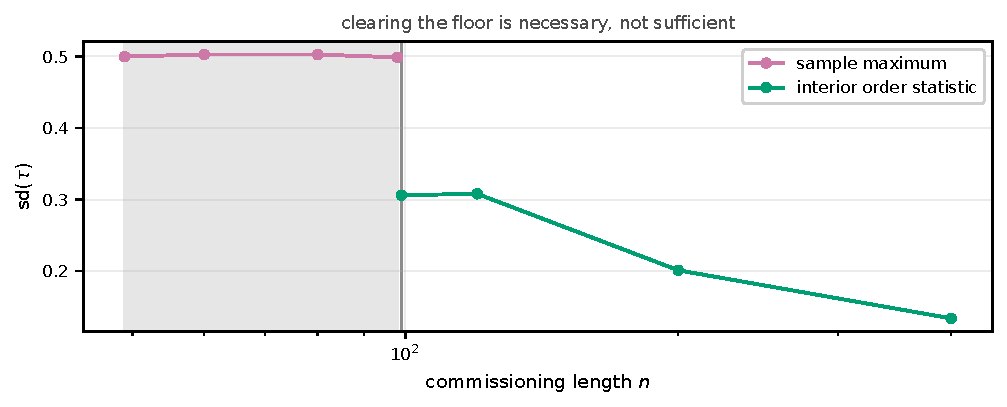
\includegraphics[width=\linewidth]{figures/estimator_variance}
\caption{Dispersion of the certified radius against commissioning length. The
shaded region is the degenerate range of
Corollary~\ref{cor:degenerate_range} and the vertical rule the first length
admitting an interior order statistic. The gap between the two curves is not
missing data: the estimator changes identity there, from the sample maximum to
an interior order statistic, and only then does its dispersion begin to
contract. Generated by \texttt{experiments/make\_figures.py}.}
\label{fig:variance}
\end{figure}

Figure~\ref{fig:variance} shows the consequence directly. The dispersion is
flat to within \(1\%\) across \([49,98]\) and then falls by
a factor of \(1.6\) at the first interior order statistic and by \(2.5\) by
\(n=200\). Clearing the commissioning floor is therefore necessary but not
sufficient: a commissioning length chosen just above \(49\) satisfies
Corollary~\ref{cor:min_commissioning} while purchasing the most variable
estimator available.

\paragraph{The exchangeability test.}
Table~\ref{tab:exchangeability} reports its size and power. The size column
lies between \(0.025\) and \(0.083\) against a nominal \(0.05\), within the
binomial standard error of \(0.0199\) at \(120\) trials, and shows no
systematic dependence on the distribution, as a rank-based statistic requires.
Power rises monotonically with the injected drift and reaches unity at two
standard deviations of accumulated trend in five of six cases. The test is
therefore usable as a probe of Assumption~\ref{ass:exchangeability} rather
than as a source of spurious alarms.

% GENERATED by experiments/make_tables.py -- do not edit.
% source: results/data.json, run 2026-07-31T13:28:42.592521+00:00, seed 20260730
% regenerate: python3 run_all.py && python3 make_tables.py
% label: tab:exchangeability
\begin{table}[htbp]
\centering
\caption{Rejection rate of the permutation test at level $0.05$. The first
column is the size, measured on exchangeable streams; the remainder is the
power against an injected monotone drift, in standard deviations of
accumulated trend.}
\label{tab:exchangeability}
\begin{tabular}{lrrrrr}
\toprule
Residual distribution & size & drift 0.5 & drift 1.0 & drift 2.0 & drift 3.0 \\
\midrule
lognormal(0,0.4) & 0.042 & 0.133 & 0.692 & 1.000 & 1.000 \\
gamma(k=3) & 0.058 & 0.233 & 0.692 & 1.000 & 1.000 \\
exponential(1) & 0.042 & 0.408 & 0.825 & 1.000 & 1.000 \\
pareto(a=3) & 0.025 & 0.683 & 0.992 & 1.000 & 1.000 \\
halfnormal & 0.083 & 0.208 & 0.592 & 0.992 & 1.000 \\
bimodal mixture & 0.042 & 0.525 & 0.875 & 1.000 & 1.000 \\
\bottomrule
\end{tabular}
\end{table}


%---------------------------------------------------------------------
\subsection{Controlled instantiation on the simulator}
\label{subsec:results_simulator}
%---------------------------------------------------------------------

\paragraph{The representation operator and its training.}
The operator is the convolutional autoencoder of the technical note,
reproduced without modification at \(847{,}601\) trainable parameters and
fitted on \(4000\) simulated nominal windows. The epoch count is a budget
rather than a target: training is stopped by validation loss, the learning
rate is annealed on plateaus, and the best weights are restored. On the run
reported here it terminated after \(372\) of a permitted \(500\) epochs, with
the best validation loss of \(2.62\times10^{-3}\) attained at epoch \(347\)
and the learning rate annealed from \(10^{-3}\) to \(2\times10^{-6}\) in nine
reductions. Validation uses a held-out split of the \emph{nominal} data only,
so early stopping selects for reconstructing nominal behaviour and cannot
consult a fault.

One operator, trained once, is used for every experiment in this subsection.
Deterministic kernels are enabled throughout.

\paragraph{End-to-end membership.}
With the radius certified from \(120\) nominal windows, the held-out
false-alarm rate on \(1500\) further nominal windows is \(\etoeFAR\%\)
against a nominal \(2\%\). The median residual rises from \(2.32\times10^{-3}\) on
nominal windows to \(6.88\times10^{-3}\), \(1.08\times10^{-2}\) and
\(1.73\times10^{-2}\) on ball, outer-race and inner-race faults, and the
single membership rule \eqref{eq:decision_rule} detects them at \(91.5\%\),
\(100\%\) and \(100\%\) respectively. No fault observation entered the
fitting, the calibration or the stopping decision.

Four simulated assets differing only by an installation signature, sharing one
representation operator and one target coverage, identify radii of
\(1.00\times10^{-2}\), \(8.26\times10^{-3}\), \(2.45\times10^{-2}\) and
\(1.43\times10^{-2}\), a spread of \(2.97\) between the largest and the
smallest. This is the behaviour Remark~\ref{rem:scale_not_invariant}
predicts: the representation is shared and its residual scale is not.

\paragraph{Intrinsic dimension of the nominal cloud.}
Table~\ref{tab:dimension} tests the prediction of
Remark~\ref{rem:nuisance_on_attractor} that each nuisance parameter acting
non-trivially contributes one direction to the nominal set.

% GENERATED by experiments/make_tables.py -- do not edit.
% source: results/data.json, run 2026-07-31T13:28:42.592521+00:00, seed 20260730
% regenerate: python3 run_all.py && python3 make_tables.py
% label: tab:dimension
\begin{table}[htbp]
\centering
\caption{Maximum-likelihood intrinsic dimension \citep{levina2004} of the
noise-free nominal family, against the number of active nuisance parameters,
at three neighbourhood sizes $k$. The estimator is biased downward,
increasingly so with dimension, so the criterion is whether it
\emph{tracks} the prediction rather than whether it matches it. Ambient
dimension is 1200.}
\label{tab:dimension}
\begin{tabular}{lrrrr}
\toprule
active nuisance parameters & predicted & $k=10$ & $k=20$ & $k=40$ \\
\midrule
amplitude & 1 & 1.00 & 1.00 & 0.99 \\
amplitude+phase & 2 & 1.97 & 1.95 & 1.94 \\
amplitude+phase+speed & 3 & 2.88 & 2.85 & 2.80 \\
all four & 4 & 3.68 & 3.59 & 3.48 \\
phase+speed+offset & 3 & 2.84 & 2.76 & 2.70 \\
speed+offset & 2 & 1.93 & 1.92 & 1.91 \\
\bottomrule
\end{tabular}
\end{table}


The estimator is the maximum-likelihood construction of \citet{levina2004},
evaluated at several neighbourhood sizes \(k\) and combined by averaging the
inverse estimates rather than the estimates themselves, which is the
correction of \citet{mackay2005dimension} and removes the strong bias the
original averaging exhibits at small \(k\).

Each additional parameter raises the estimate by close to one, and the
single-parameter case is recovered exactly. The residual gap grows with the
dimension, which is the downward bias documented for this estimator on
manifolds of increasing dimension rather than an unexplained discrepancy; a
mistaken reading would fail to track the count at
all. Figure~\ref{fig:dimension} shows the tracking directly.

Additive noise thickens the cloud without adding dimension, and the estimator
shows this as scale dependence: on the full simulator the estimate falls from
about twelve at the smallest neighbourhood to close to four at the largest,
approaching the noise-free values. Against an ambient dimension of \(1200\),
an intrinsic dimension near four is what makes the covering argument of
Remark~\ref{rem:fill_rate} usable rather than vacuous, and it is measured here
rather than assumed.

\begin{figure}[htbp]
\centering
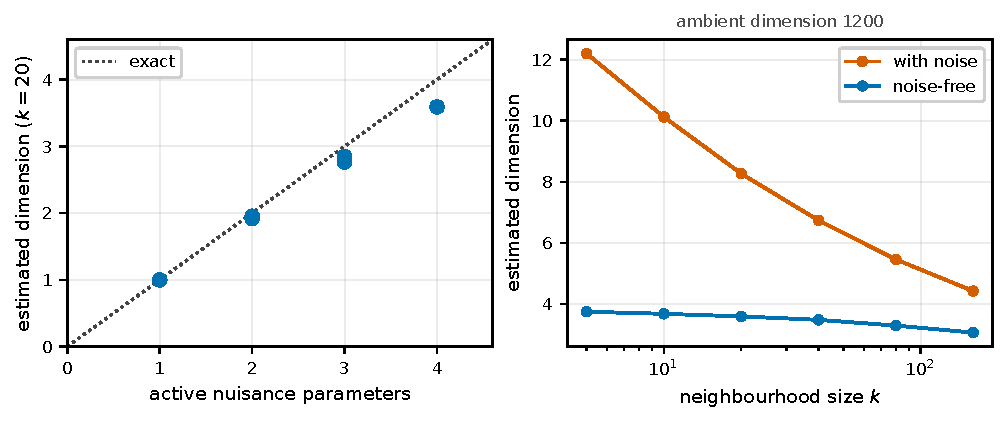
\includegraphics[width=\linewidth]{figures/intrinsic_dimension}
\caption{Intrinsic dimension of the nominal cloud. Left: the estimate against
the number of nuisance parameters actually varied, with the diagonal marking
exact recovery; the estimator tracks the count with a downward bias that grows
with dimension. Right: scale dependence on the full simulator, where additive
noise raises the estimate at small neighbourhoods and the manifold structure
emerges as the neighbourhood grows. Generated by
\texttt{experiments/make\_figures.py}.}
\label{fig:dimension}
\end{figure}

\paragraph{Attractor drift under slow parameter change.}
On chronological records of \(700\) windows whose first half is nominal and
whose severity then ramps smoothly, the radius is commissioned on the
early-life segment, frozen, and never adapted. Departure is declared by a
persistence rule. Onset occurs at record \(351\); persistent departure is
declared at \(473\), \(496\) and \(545\) for inner-race, outer-race and ball
faults, delays of \(122\), \(145\) and \(194\) records, at severities of
\(0.211\), \(0.251\) and \(0.335\) on a ramp reaching \(0.6\). Post-departure
exceedance is \(96.1\%\), \(98.2\%\) and \(96.8\%\).
Figure~\ref{fig:drift} shows the trajectories.

The false-alarm rate measured after commissioning but before onset, where the
process is still nominal, is \(5.2\%\) against the \(2\%\) target. This is
higher than the calibrated level and is worth stating: it is measured on a
single realisation over roughly \(230\) records, so its sampling error is
substantial, but it also reflects that the commissioning segment and the later
nominal segment are not perfectly exchangeable in a record that will
subsequently degrade. It is the same assumption,
Assumption~\ref{ass:exchangeability}, that the permutation test of
Section~\ref{subsec:results_verification} is designed to probe.

What the detector is given is no severity information, no fault label and no
adaptation after commissioning. What it reports is failure of membership in a
region estimated before any degradation occurred, which is the distinction
drawn in Section~\ref{subsec:disc_dynamics} between motion along a fixed orbit
and motion of the orbit itself.

\begin{figure}[htbp]
\centering
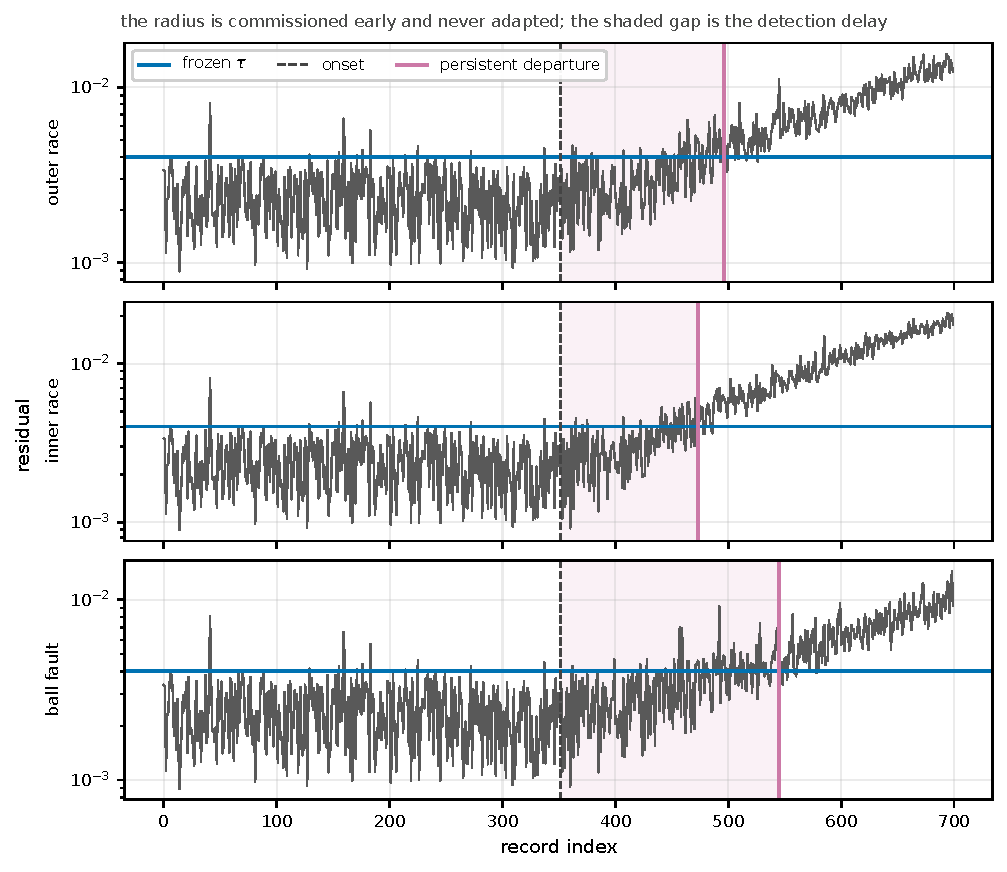
\includegraphics[width=\linewidth]{figures/degradation_trajectory}
\caption{Degradation trajectories under a frozen radius. The horizontal line
is the radius commissioned on the early-life segment and never afterwards
adapted; the dashed line marks the onset of non-zero severity and the solid
vertical line the first persistent departure, with the shaded interval the
detection delay. Generated by \texttt{experiments/make\_figures.py}.}
\label{fig:drift}
\end{figure}

\paragraph{Saturation of the nominal radius.}
Table~\ref{tab:saturation} measures the radius of
Definition~\ref{def:saturation_radius} against a reference estimated from
\(\satRefWindows\) held-out nominal windows. Attained coverage is measured on
a fresh evaluation block of \(\satEvalBlock\) windows drawn, disjointly from
the calibration draw, on each of the \(\satReps\) repetitions. The choice is
not a detail. Holding a single evaluation block fixed estimates coverage
against that block's empirical distribution function rather than against the
distribution, an offset of order \(\sqrt{p(1-p)/M}\) that does not average
away over repetitions and is of the same order as the excess coverage being
reported. Drawing calibration and evaluation points jointly without
replacement from one pool is moreover not an approximation to independent
sampling: the pool is exchangeable, so any \(n+1\) of its members drawn
without replacement are exchangeable, which is the sole hypothesis of
Proposition~\ref{prop:coverage}.

% GENERATED by experiments/make_tables.py -- do not edit.
% source: results/data.json, run 2026-07-31T13:28:42.592521+00:00, seed 20260730
% regenerate: python3 run_all.py && python3 make_tables.py
% label: tab:saturation
\begin{table}[htbp]
\centering
\caption{Saturation of the nominal radius against the reference
$R_p=22.599$. ``certified'' is the estimator of
Corollary~\ref{cor:saturation_certification}, ``interp'' the interpolated
empirical quantile. ``exact'' is the coverage predicted by
Proposition~\ref{prop:coverage}, $k_\alpha/(n+1)$; the observed certified
coverage matches it to within 1.1 Monte Carlo
standard errors at every $n$, including the non-trivial values taken inside the
degenerate range. The interpolated estimator undercovers throughout. A dash
marks a commissioning length below the floor, at which no radius is
certifiable.}
\label{tab:saturation}
\setlength{\tabcolsep}{4pt}\small
\begin{tabular}{rrrrrrrrl}
\toprule
$n$ & certified & sd & bias (\%) & coverage & exact & interp & int.\ cov & max? \\
\midrule
30 & -- & -- & -- & -- & -- & 21.109 & 0.9499 & -- \\
49 & 23.106 & 1.606 & $+2.24$ & 0.9801 & 0.9800 & 21.570 & 0.9611 & yes \\
60 & 23.613 & 1.726 & $+4.49$ & 0.9841 & 0.9836 & 21.708 & 0.9655 & yes \\
80 & 23.860 & 1.522 & $+5.58$ & 0.9868 & 0.9877 & 21.974 & 0.9683 & yes \\
98 & 24.110 & 1.534 & $+6.69$ & 0.9889 & 0.9899 & 22.019 & 0.9706 & yes \\
99 & 22.917 & 1.300 & $+1.41$ & 0.9805 & 0.9800 & 22.084 & 0.9704 & no \\
150 & 22.812 & 0.993 & $+0.94$ & 0.9805 & 0.9801 & 22.216 & 0.9736 & no \\
300 & 22.671 & 0.723 & $+0.32$ & 0.9795 & 0.9801 & 22.388 & 0.9763 & no \\
800 & 22.619 & 0.407 & $+0.09$ & 0.9799 & 0.9800 & 22.518 & 0.9786 & no \\
2000 & 22.584 & 0.225 & $-0.07$ & 0.9794 & 0.9800 & 22.538 & 0.9789 & no \\
\bottomrule
\end{tabular}
\end{table}


\begin{figure}[htbp]
\centering
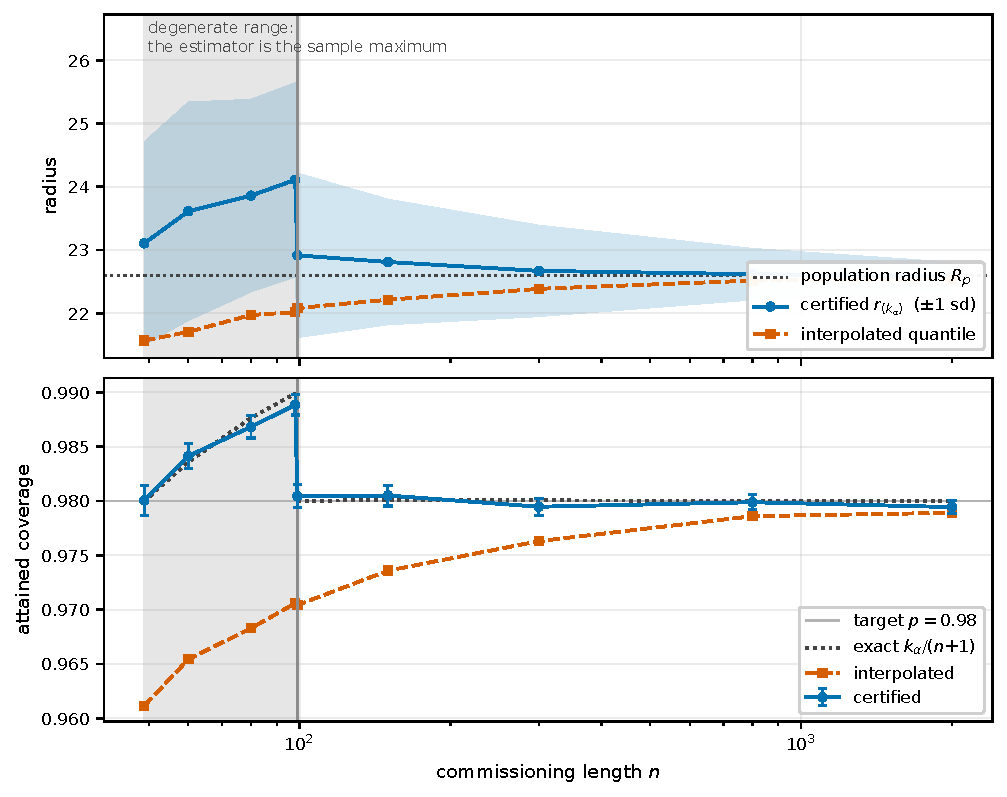
\includegraphics[width=\linewidth]{figures/saturation}
\caption{Saturation of the nominal radius. Upper panel: the certified radius
with a $\pm 1$ standard-deviation band, against the population value; the
shaded region is the degenerate range of
Corollary~\ref{cor:degenerate_range}, in which the estimator is the sample
maximum and therefore rises with $n$ rather than settling, and the vertical
rule marks the first commissioning length admitting an interior order
statistic. Lower panel: attained coverage, with Monte Carlo error bars. The
dotted reference is not the target level but the exact coverage
\(k_\alpha/(n+1)\) of Proposition~\ref{prop:coverage}, which exceeds the
target and is not monotone in \(n\); the certified curve tracks it, while the
interpolated estimator produces the smooth radius curve above and undercovers
at every length examined. Generated by
\texttt{experiments/make\_figures.py}.}
\label{fig:saturation}
\end{figure}

Four things follow from Table~\ref{tab:saturation} and
Figure~\ref{fig:saturation}, and the first three are the substance of
Remark~\ref{rem:saturation_tension}.

First, the certified coverage agrees with the exact value
\(k_\alpha/(n+1)\) at every commissioning length on the grid, to within
\(\satMaxZ\) Monte Carlo standard errors. This is a sharper statement than the
inequality \(\text{coverage}\ge p\), and it is the sharper statement that is
worth making: \(k_\alpha/(n+1)\) is not monotone in \(n\) and takes distinctly
non-trivial values inside the degenerate range, where it rises to
\(\satExactAtDegHi\) at \(n=98\) against an observed \(\satCovAtDegHi\). An
estimator that merely covered conservatively would satisfy the inequality
while missing that structure entirely.

Second, inside the degenerate range the certified radius does not settle: its
mean drifts from \(\satBiasLo\%\) above \(R_p\) at \(n=49\) to
\(\satBiasHi\%\) at \(n=98\), and then falls discontinuously to
\(\satBiasDrop\%\) at \(n=99\), where an interior order statistic first
becomes available. This is not a property of the regime but of the estimator,
which is the sample maximum throughout that band by
Corollary~\ref{cor:degenerate_range}. A saturation curve computed this way
cannot flatten there, and apparent settling is the maximum of a growing
sample. The excess coverage inside the band is the same fact stated in the
other coordinate: covering more than the target is precisely what a radius
that is too large does.

Third, the interpolated estimator behaves in the complementary way. It
approaches \(R_p\) smoothly from below, producing the familiar saturating
curve, and its coverage is below the \(p=0.98\) target at every commissioning
length examined, from \(\satInterpFirstCov\) at \(n=\satInterpFirstN\) to
\(\satInterpLastCov\) at \(n=\satInterpLastN\). The visual impression of
convergence and the coverage guarantee are supplied by different estimators,
and not by the same one.

Fourth, replacing the split-sample reference by a plug-in reference fitted on
the same observations shrinks the radius by \(\satPlugShiftLo\) to
\(\satPlugShiftHi\%\) at \(n\in\{\satPlugGrid\}\), confirming the sign
predicted in Remark~\ref{rem:plugin_centroid}. Coverage, however, is not degraded, because
the evaluation distances are recomputed in the same plug-in geometry and the
two shift together. The practical cost of a plug-in reference is therefore the
comparability of radii across assets and regimes, not the validity of the
membership test, and the remark is refined accordingly.

\paragraph{A negative result: the radius is not a detector.}
Measured under the shared nominal projection, the certified radius of each
regime is \(\satRadiusNom\) for nominal, \(\satRadiusOuter\) for outer-race,
\(\satRadiusInner\) for inner-race and \(\satRadiusBall\) for ball faults,
that is, ratios to nominal between \(\satRatioLo\) and \(\satRatioHi\). There
is no separation. The explanation is mechanical: a two-dimensional principal
projection of a raw vibration window is dominated by the shaft harmonics,
while the fault signature is a low-amplitude impulse train contributing almost
nothing to the leading variance directions. The same simulator, the same
nominal-only fitting and the same membership rule detect those faults at
\(\etoeDetectLo\)--\(\etoeDetectHi\%\) when the residual is used instead.
Saturation of a region and separability of that region from its neighbours are
therefore independent properties, as
Remark~\ref{rem:radius_not_detector} states, and a saturation plot is evidence
about the sampling of the nominal geometry rather than about regime
discrimination.

\paragraph{Operator adequacy: coverage cannot choose between residuals.}
Table~\ref{tab:adequacy} applies the probe of
Remark~\ref{rem:level_not_shape} to two operators calibrated identically on
the same nominal data, at the same target coverage.

% GENERATED by experiments/make_tables.py -- do not edit.
% source: results/data.json, run 2026-07-31T13:28:42.592521+00:00, seed 20260730
% regenerate: python3 run_all.py && python3 make_tables.py
% label: tab:adequacy
\begin{table}[htbp]
\centering
\caption{Distance-proxy probe. Latent codes are pushed away from the nominal
range, decoded, and the residual compared against the true distance to a
disjoint nominal cloud, whose median nearest-neighbour spacing is
3.04. Both operators attain the calibrated coverage; they differ by
more than two orders of magnitude in what they accept.}
\label{tab:adequacy}
\setlength{\tabcolsep}{5pt}
\begin{tabular}{lrrrrl}
\toprule
operator & healthy FAR & ball DR & max accepted & ratio to & adequacy \\
         & (\%)        & (\%)    & distance     & spacing  &          \\
\midrule
PCA-16 & 2.0 & 84 & $1.16e+03$ & $381.6\times$ & fail \\
Conv1D AE & 2.3 & 90 & $4.98$ & $1.6\times$ & pass \\
\bottomrule
\end{tabular}
\end{table}


\begin{figure}[htbp]
\centering
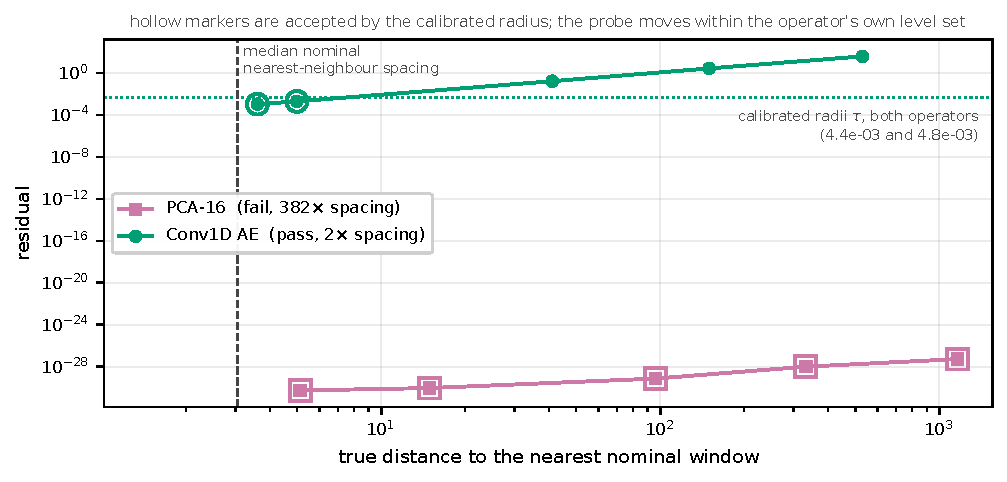
\includegraphics[width=\linewidth]{figures/distance_proxy_probe}
\caption{The distance-proxy probe. Latent codes are pushed away from the
nominal range, decoded, and the resulting residual plotted against the true
distance to a disjoint nominal cloud; hollow markers are points the calibrated
radius accepts. Both axes are logarithmic because the two operators differ by
some thirty orders of magnitude in residual and two in accepted distance. The
two calibrated radii nearly coincide, which is the point: identical
calibration data and an identical target coverage give almost the same
threshold, and the operators nevertheless accept points that are twenty-five
orders of magnitude apart in residual and two apart in true distance.
Generated by \texttt{experiments/make\_figures.py}.}
\label{fig:adequacy}
\end{figure}

Figure~\ref{fig:adequacy} makes the separation visible. The linear operator
accepts a point at \(1160\) units from the nearest nominal
window, some \(380\) times the nominal spacing, while assigning it a residual
of order \(10^{-28}\). Its accepted region is a slab around the retained
subspace, not a tube around the nominal manifold, exactly as
Remark~\ref{rem:level_not_shape} anticipates for a residual that measures
distance to a structure containing the nominal set rather than to the set.
The convolutional operator rejects everything beyond \(1.6\) times the
spacing, and its residual rises from \(1.08\times10^{-3}\) to \(38.6\) across
the probe, a growth of four orders of magnitude.

The comparison is informative precisely because detection does not separate
the two. Both reach \(100\%\) on outer- and inner-race faults, and the linear
operator reaches \(84\%\) on ball faults against \(90\%\) for the
convolutional one. A reader judging by detection rates alone would find them
comparable. Coverage does not separate them either, by
Proposition~\ref{prop:coverage}, which holds for both. Only the probe does,
and the property it detects is the one on which tightness depends. This is the
empirical content of the claim that this work certifies the level and inherits
the shape.

%---------------------------------------------------------------------
\subsection{Field transfer: CWRU}
\label{subsec:results_cwru}
%---------------------------------------------------------------------

The results in this subsection and the next are carried over from the existing
pipeline and are not regenerated by the accompanying package, for the reasons
given in Section~\ref{subsec:design_reproducibility}. By
Section~\ref{subsec:design_caveat} they were obtained with the interpolated
estimator and \(N_{\min}=40\), that is, in the A1 configuration, and therefore
do not carry the guarantee of Proposition~\ref{prop:coverage}.

Table~\ref{tab:cwru_oracle} establishes the reference. Independently trained
asset-specific detectors, one representation and one preprocessing
transformation per operating condition fitted on that condition's complete
healthy record, achieve \(100\%\) detection for all three fault families at a
mean healthy false-alarm rate of \(2.29\pm 0.12\%\). Their absolute decision
thresholds range from \(0.459\) to \(0.759\), a spread of \(1.65\), although
their diagnostic operating points are identical. Numerical residual scales are
not interchangeable even between models of the same architecture trained on
the same data, which is
Remark~\ref{rem:scale_not_invariant} in its sharpest form.

\begin{table}[!ht]
\centering
\caption{Asset-specific reference on CWRU. Each detector is trained and
calibrated independently on the complete healthy record of its operating
condition. This reference is deliberately favourable and operationally
unavailable.}
\label{tab:cwru_oracle}
\begin{tabular}{lrrrrr}
\toprule
RPM & threshold & healthy FAR (\%) & ball DR (\%) & inner DR (\%) & outer DR (\%) \\
\midrule
1730 & 0.6485 & 2.23 & 100.00 & 100.00 & 100.00 \\
1750 & 0.7590 & 2.23 & 100.00 & 100.00 & 100.00 \\
1772 & 0.7248 & 2.23 & 100.00 & 100.00 & 100.00 \\
1797 & 0.4591 & 2.46 & 100.00 & 100.00 & 100.00 \\
\midrule
mean & --     & $2.29\pm0.12$ & $100.00$ & $100.00$ & $100.00$ \\
\bottomrule
\end{tabular}
\end{table}

Table~\ref{tab:cwru_transfer} reports the three calibration strategies under
one shared simulator-trained representation.

\begin{table}[!ht]
\centering
\caption{Simulation-to-field transfer on CWRU under one shared
representation. Only the information available for estimating the radius
differs between strategies. Healthy FAR covers the complete healthy sequence
including commissioning observations; post-convergence values appear in
Table~\ref{tab:cwru_agreement}.}
\label{tab:cwru_transfer}
\setlength{\tabcolsep}{4pt}
\begin{tabular}{llrrrrrr}
\toprule
RPM & calibration & \(\tau\) & FAR (\%) & ball (\%) & inner (\%) & outer (\%) & windows \\
\midrule
1730 & direct transfer & 0.1027 & 100.00 & 100.00 & 100.00 & 100.00 & -- \\
1730 & field oracle    & 0.3578 & 2.23   & 99.75  & 100.00 & 99.86  & -- \\
1730 & online          & 0.3520 & 3.71   & 99.75  & 100.00 & 100.00 & 49 \\
\addlinespace
1750 & direct transfer & 0.1027 & 100.00 & 100.00 & 100.00 & 100.00 & -- \\
1750 & field oracle    & 0.3434 & 2.23   & 100.00 & 100.00 & 100.00 & -- \\
1750 & online          & 0.3440 & 1.98   & 100.00 & 100.00 & 100.00 & 62 \\
\addlinespace
1772 & direct transfer & 0.1027 & 100.00 & 100.00 & 100.00 & 100.00 & -- \\
1772 & field oracle    & 0.3512 & 2.23   & 100.00 & 100.00 & 100.00 & -- \\
1772 & online          & 0.3550 & 1.24   & 100.00 & 100.00 & 100.00 & 58 \\
\addlinespace
1797 & direct transfer & 0.1027 & 100.00 & 100.00 & 100.00 & 100.00 & -- \\
1797 & field oracle    & 0.3886 & 2.46   & 98.03  & 100.00 & 100.00 & -- \\
1797 & online          & 0.3869 & 3.45   & 98.52  & 100.00 & 100.00 & 49 \\
\bottomrule
\end{tabular}
\end{table}

Direct transfer of the absolute simulator threshold fails under every
operating condition, flagging every healthy window as anomalous while
producing an apparent \(100\%\) detection rate. This is the predicted outcome
of Remark~\ref{rem:scale_not_invariant} and is the empirical content of the
claim that the representation transfers and its scale does not: the same
representation, given a locally estimated radius, recovers an operationally
meaningful boundary in the same table.

Local calibration does exactly that. The complete-data field oracle reproduces
the expected \(2\%\) operating point, and the online procedure reaches a
comparable one after \(49\), \(62\), \(58\) and \(49\) observations, a mean of
\(54.5\pm 6.6\). Table~\ref{tab:cwru_agreement} compares the converged radii
with the oracle values.

\paragraph{How generous the oracle is, and why that strengthens the comparison.}
The oracle is an upper bound in the strong sense: it fits its representation
on an asset's complete healthy record and then calibrates its threshold on
that same record, with nothing held out. It is not a deployable procedure and
is not offered as one. What is worth quantifying is how much that costs in
optimism, because the online arm is being asked to match it.

Refitting the four asset-specific operators shows that they do not merely use
all the data, they memorise it: the validation loss exceeds the training loss
by factors of \(2.4\), \(3.9\), \(3.2\) and \(1.5\) across the four speeds,
for \(847{,}601\) parameters fitted to roughly \(320\) training windows. A
threshold calibrated on those same windows therefore sits at the \(98\)th
percentile of residuals the operator has partly reconstructed from memory,
and the resulting \(2.23\%\) false-alarm rate is optimistic by construction.

The online arm has no such advantage. It calibrates on a chronological prefix
and is evaluated on what follows, so its false-alarm rate is measured on
observations the radius never saw. Read against that, the comparison in
Table~\ref{tab:cwru_transfer} is stronger than parity: the online procedure
matches the oracle's detection at every speed, exceeds it on ball faults at
\(1797\,\mathrm{RPM}\) (\(98.52\%\) against \(98.03\%\)), and attains a LOWER
false-alarm rate at two of the four speeds (\(1.98\%\) against \(2.23\%\), and
\(1.24\%\) against \(2.23\%\)) --- while using fifty-odd observations against
four hundred, and while the reference it is being measured against is the one
allowed to see the answers.

Two details of that table are also explained by sample size rather than by
anything about the assets. The healthy record at \(1797\,\mathrm{RPM}\) is
half the length of the other three, \(203\) windows against about \(404\),
which makes its \(98\)th percentile the fourth-largest order statistic rather
than the eighth and fixes its attained false-alarm rate at \(2.46\%\) rather
than \(2.23\%\). Truncating the other three speeds to \(203\) windows
reproduces \(2.46\%\) at all four, so the difference is arithmetic of the
estimator and not a property of that operating condition. Its threshold is
also the lowest of the four, which is a separate and benign fact: the healthy
record at that speed is the most homogeneous of the four --- the only one whose
operator does not memorise, at a validation-to-training ratio of \(1.5\) ---
so a tighter radius is the correct outcome rather than an anomalous one.

\begin{table}[!ht]
\centering
\caption{Agreement between the converged online radius and the complete-data
oracle. Post-calibration FAR is evaluated only on healthy observations
occurring after the declared convergence point.}
\label{tab:cwru_agreement}
\begin{tabular}{lrrrrr}
\toprule
RPM & \(\tau_{\mathrm{oracle}}\) & \(\tau_{\mathrm{online}}\) & rel.\ diff.\ (\%) & windows & post-cal.\ FAR (\%) \\
\midrule
1730 & 0.3578 & 0.3520 & 1.64 & 49 & 3.94 \\
1750 & 0.3434 & 0.3440 & 0.19 & 62 & 1.75 \\
1772 & 0.3512 & 0.3550 & 1.06 & 58 & 0.87 \\
1797 & 0.3886 & 0.3869 & 0.44 & 49 & 3.90 \\
\midrule
mean & --     & --     & 0.83 & $54.5\pm6.6$ & 2.62 \\
\bottomrule
\end{tabular}
\end{table}

The converged radii differ from their oracle references by
\(0.19\)--\(1.64\%\), a mean of \(0.83\%\). The procedure therefore recovers
nearly the same acceptance boundary that retrospective access to the complete
healthy record would have produced, from at most \(62\) observations.

\paragraph{The commissioning lengths, and what they do not show.}
The four commissioning lengths are \(49\), \(62\), \(58\) and \(49\), and the
coverage floor of Corollary~\ref{cor:min_commissioning} at
\(\alpha=0.02\) is also \(49\). By
Remark~\ref{rem:49_confound} these coincide for unrelated reasons: the
stopping rule cannot emit a length below \(49\) at the configuration used, and
that bound does not involve \(\alpha\). The clustering is therefore
uninformative about the floor, and is reported here only to forestall the
inference.

More consequentially, all four lengths lie in \([49,98]\), which by
Corollary~\ref{cor:degenerate_range} is the range in which a certified radius
would be the sample maximum. Combined with the use of an interpolated
quantile, this places the field calibration in precisely the regime that
Table~\ref{tab:saturation} characterizes as simultaneously the most variable
and the least conservative.

\paragraph{Robustness, read as a probe of exchangeability.}
Permuting the commissioning observations and their arrival order over five
realizations per condition, with the representation and all parameters fixed,
gives \(20\) convergent runs out of \(20\). The estimated radius stays within
\(2.08\pm0.71\%\) of the oracle and the fleet-averaged post-calibration
false-alarm rate is \(3.59\pm1.59\%\). Following
Remark~\ref{rem:exchangeability_test}, the absence of systematic dependence on
arrival order is the evidence bearing on
Assumption~\ref{ass:exchangeability}, and it is consistent with the assumption
holding within the commissioning window.

The dispersion is nonetheless substantial: one \(1750\,\mathrm{RPM}\)
realization produced a post-calibration false-alarm rate of \(13.8\%\) while
remaining within \(4\%\) of the oracle radius. This is finite-sample
uncertainty in an extreme quantile estimated inside the degenerate range, and
Table~\ref{tab:variance} gives its scale directly: at \(n\approx 55\) the
estimator has the same dispersion as at \(n=49\), and \(2.5\) times that
available at \(n=200\).

\paragraph{Cost of sharing one representation.}
Relative to the asset-specific reference of
Table~\ref{tab:cwru_oracle}, replacing four independently trained detectors by
one simulator-trained representation with local calibration changes mean
ball-fault detection from \(100.00\pm0.00\%\) to \(99.57\pm0.71\%\), leaves
inner- and outer-race detection at \(100\%\), and raises the mean healthy
false-alarm rate from \(2.29\pm0.12\%\) to \(2.60\pm1.18\%\). The reference
requires a fitted preprocessing transformation, a trained representation and
the complete healthy record of every condition; the shared alternative
requires \(49\)--\(62\) nominal observations and no field training.

%---------------------------------------------------------------------
\subsection{Field transfer: NASA IMS}
\label{subsec:results_nasa}
%---------------------------------------------------------------------

Table~\ref{tab:nasa} reports the four run-to-failure bearings, and
Figure~\ref{fig:nasa} shows the trajectories they were read from.

% GENERATED by experiments/make_tables.py -- do not edit.
% source: results/data.json, run 2026-07-31T13:28:42.592521+00:00, seed 20260730
% regenerate: python3 run_all.py && python3 make_tables.py
% label: tab:nasa
\begin{table}[htbp]
\centering
\caption{NASA IMS deployment under one shared simulator-trained
representation with local radius estimation. Relative error is against the
complete-data reference for that bearing; lead time is measured to the end of
the usable record. The final 2 recordings of the archive were taken with
the rig stopped and are excluded (see Section~\ref{subsec:results_nasa}).
Radii span a factor of 2.24 under an identical
representation, target coverage and stopping rule. Generated by
\texttt{experiments/make\_tables.py} from the committed residual cache.}
\label{tab:nasa}
\setlength{\tabcolsep}{5pt}
\begin{tabular}{lrrrrr}
\toprule
Bearing & windows & \(\tau_k\) & rel.\ error (\%) & post-dep.\ exceedance (\%) & lead time (h) \\
\midrule
1 & 49 & 0.014150 & 0.21 & 100.00 & 73.83 \\
2 & 54 & 0.018596 & 0.70 & 93.09 & 31.33 \\
3 & 49 & 0.021798 & 2.24 & 100.00 & 14.33 \\
4 & 49 & 0.009729 & 0.20 & 94.92 & 52.50 \\
\midrule
mean & 50 & -- & 0.84 & 97.00 & 43.00 \\
\bottomrule
\end{tabular}
\end{table}


\begin{figure}[htbp]
\centering
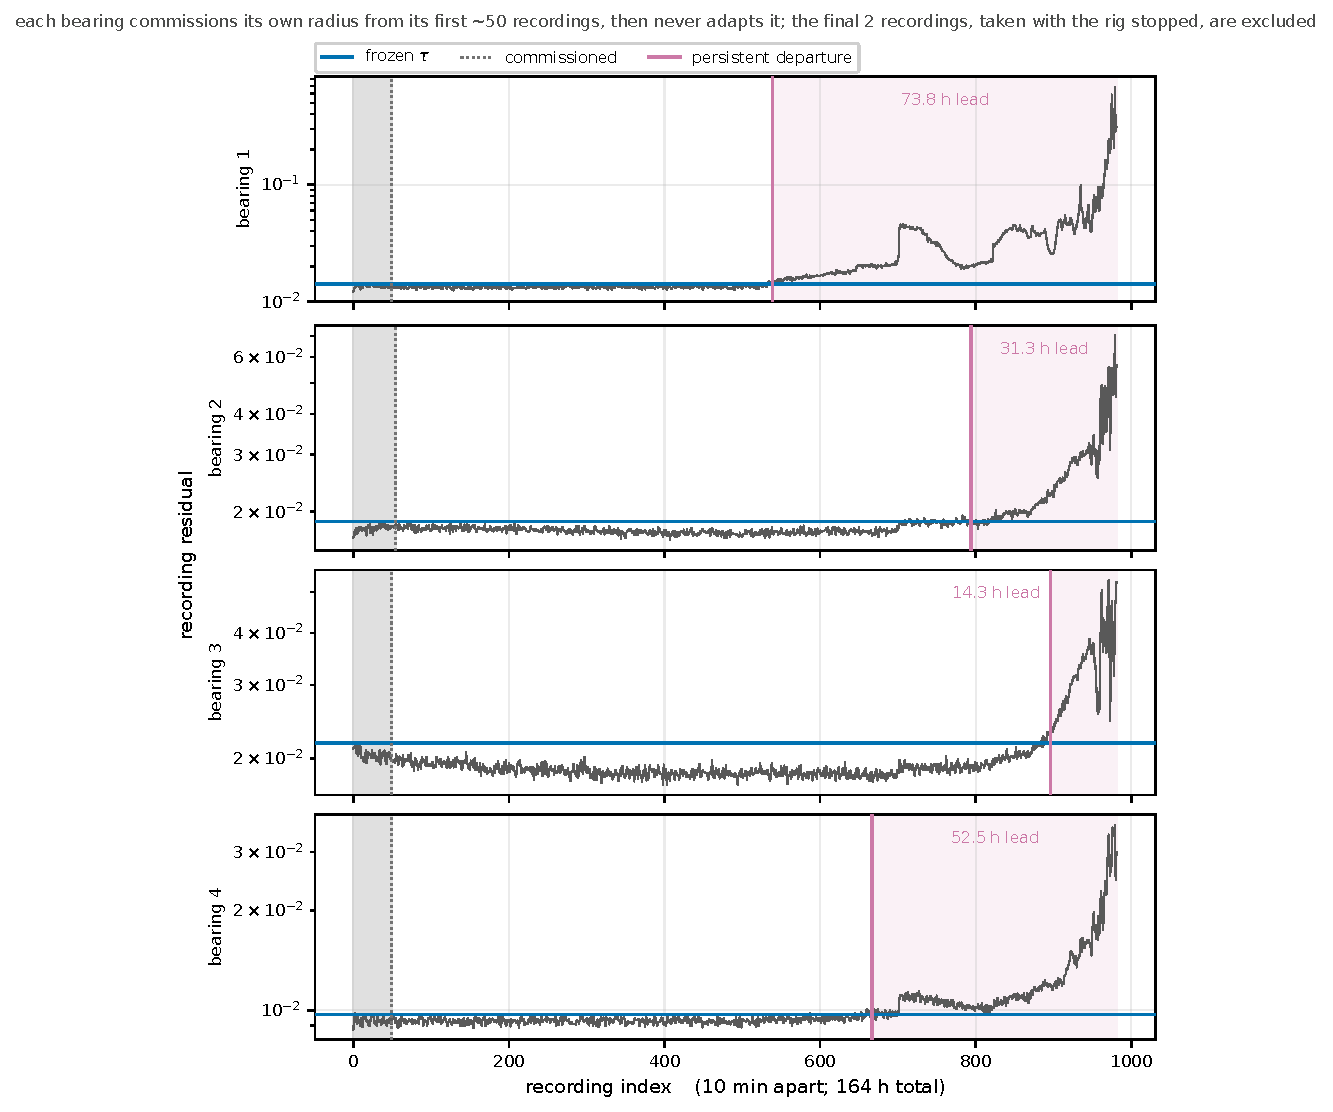
\includegraphics[width=\linewidth]{figures/nasa_trajectories}
\caption{NASA IMS run-to-failure trajectories under one shared
simulator-trained representation. Each panel is one bearing's recording-level
residual over the complete \(164\)-hour record. The shaded prefix is the
early-life segment from which that bearing commissions its own radius; the
dotted rule is where the convergence criterion stopped it, near fifty
recordings out of nine hundred and eighty-four. The horizontal line is the
radius, frozen at that point and never adapted. The vertical rule is the first
persistent departure under the eight-of-ten rule, and the shaded interval to
its right is the lead time. The final two recordings of the archive were taken
with the rig stopped --- signal standard deviation near \(0.001\) against
\(0.13\)--\(0.48\) while running --- and are excluded rather than plotted,
since on a logarithmic axis they produce a cliff that reads as a measurement
artefact. Generated by \texttt{experiments/make\_figures.py} from the
committed residual cache, so it regenerates without the archive.}
\label{fig:nasa}
\end{figure}

Calibration converged for all \(\nasaBearings\) bearings after
\(\nasaNLo\)--\(\nasaNHi\) recordings. The converged radii span
\(\nasaTauLo\) to \(\nasaTauHi\), a factor of \(\nasaTauSpread\), under
an identical representation, an identical target coverage and an identical
stopping rule. This is the same phenomenon as the
simulated assets of
Section~\ref{subsec:results_simulator} and as the CWRU threshold spread of
Table~\ref{tab:cwru_oracle}, now on physically distinct units: the
transferable object is the representation, and the radius is individual.
Corollary~\ref{cor:equivalence_class_diagnosis} is the structural statement
behind it, applied per physical unit rather than per operating condition.

All \(\nasaBearings\) bearings subsequently departed persistently from their
frozen neighbourhood, with a mean post-departure exceedance of
\(\nasaExceedanceMean\%\) and lead times of \(\nasaLeadLo\) to
\(\nasaLeadHi\) hours, a mean of \(\nasaLeadMean\). Two of the four never
re-enter their neighbourhood once they have left it, at \(100\%\)
post-departure exceedance. Repeating the
commissioning with five permuted early-life samples per bearing gave \(20\)
convergent runs out of \(20\), radii within \(0.83\%\) of their references on
average, and a healthy false-alarm rate of \(4.98\%\); bearing~3, which shows
the largest deviation in Table~\ref{tab:nasa}, is also the most sensitive to
commissioning-sample variability, at \(1.58\pm1.88\%\).

\paragraph{What the radius depends on, and what it does not.}
The radii of Table~\ref{tab:nasa} are one realisation, and the operator that
produces them is a trained network whose weights depend on an arbitrary seed.
Whether that matters is an empirical question with three candidate answers,
and it is worth separating them rather than assuming the least interesting.
Repeating the whole field pipeline under the five seeds
\(\{7,21,42,84,126\}\) --- retraining the shared operator, rescoring all
\(984\) recordings of all four bearings, recommissioning each --- gives the
following.

% GENERATED by experiments/make_tables.py -- do not edit.
% source: results/data.json, run 2026-07-31T13:28:42.592521+00:00, seed 20260730
% regenerate: python3 run_all.py && python3 make_tables.py
% label: tab:stability
\begin{table}[htbp]
\centering
\caption{Seed stability of the field pipeline. The whole chain --- retraining
the shared operator, rescoring all 984
recordings of each bearing, recommissioning --- was repeated under
5 training seeds. ``spread'' is the relative standard deviation
across seeds; ``estimator'' is the spread obtained with the operator held
FIXED and the commissioning window resampled, which isolates the contribution
of the order statistic. The decisive comparison is between the two spread
columns for $\tau$ and for $\tau$ normalised by the bearing's median
early-life residual: a seed fixes an overall gauge, not the geometry.
Monte Carlo threshold across seeds: $0.01154$ with relative spread
$7.5\%$.}
\label{tab:stability}
\setlength{\tabcolsep}{4pt}\small
\begin{tabular}{rrrrrrcc}
\toprule
 & \multicolumn{3}{c}{absolute $\tau$} & \multicolumn{2}{c}{normalised $\tau$} & & \\
\cmidrule(lr){2-4}\cmidrule(lr){5-6}
bearing & mean & spread (\%) & estimator (\%) & mean & spread (\%) & departure & lead (h) \\
\midrule
1 & 0.01310 & 5.7 & 0.5 & 1.0557 & 1.0 & 538--539 & 74.2--74.3 \\
2 & 0.01725 & 5.1 & 0.6 & 1.0401 & 0.8 & 731--794 & 31.7--42.2 \\
3 & 0.02048 & 4.4 & 1.2 & 1.1006 & 0.7 & 893--896 & 14.7--15.2 \\
4 & 0.00910 & 6.6 & 0.8 & 1.0429 & 1.2 & 662--706 & 46.3--53.7 \\
\bottomrule
\end{tabular}
\end{table}


Three things follow.

First, the radius does move with the seed, by \(4.4\) to \(6.6\%\). Reporting
it to six significant figures, as Table~\ref{tab:nasa} does for a single run,
overstates what is determined.

Second, almost none of that comes from the estimator. Holding the operator
fixed and resampling the commissioning window gives \(0.5\) to \(1.2\%\), so
the order-statistic estimator contributes between an eighth and a third of the
observed spread. This is worth stating positively: at the commissioning
lengths actually selected, near \(n=49\), the estimator is stable, which is
the empirical counterpart of clearing the degenerate range of
Corollary~\ref{cor:degenerate_range}. Nor is the spread an artefact of the
sparsity penalty on the latent layer: all \(16\) latent units remain active
under every seed, and the concentration of the code correlates with the radius
at \(+0.13\).

Third, and this is the substantive result, the variation is one of SCALE
rather than of geometry. Normalising each radius by the median early-life
residual of the same bearing under the same seed reduces the spread to
\(0.7\)--\(1.2\%\), a factor of four to nine. A seed fixes an overall gauge
for the operator: nominal and degraded residuals move together, the radius
moves with them, and the membership decision does not move at all. The
consequence is visible in the invariants. The commissioning length is \(49\)
in \(17\) of the \(20\) bearing--seed combinations, and on bearing~1 the lead
time is \(74.2\) to \(74.3\) hours across all five seeds --- a spread of
\(0.12\%\) on a seventy-four-hour forecast, produced by operators whose radii
differ by \(5.7\%\).

This is what the quotient formulation predicts and had not previously been
shown: the diagnostic content is in the geometry of the nominal region
relative to its own scale, not in the absolute value of the residual. The
radius is not a physical quantity to be reported to six digits but a
per-asset, per-operator normalisation, and its stability should be judged
after that normalisation. Where the invariance is weaker --- bearings~2 and~4,
whose departure indices range over \(63\) and \(44\) recordings against \(1\)
and \(3\) for bearings~1 and~3 --- the degradation itself is more gradual,
rising by a factor of \(1.8\) rather than \(5.6\), so the crossing of any
threshold is correspondingly less sharply timed. The stability of the
detection follows the sharpness of the fault, which is the expected ordering.

The final \(\nasaInactive\) recordings of the \(\nasaRecordings\) in the
archive are excluded from all of the above. They carry a signal whose standard
deviation is near \(0.001\) on every channel, against \(0.13\)--\(0.48\)
on the recording preceding them: the rig had been shut down. Including them
would add twenty minutes to every lead time and dilute the post-departure
exceedance with observations during which nothing was running. The experiment
ends when the operator stopped it, not when the bearing failed, and the
distinction matters for a quantity measured to the end of the record.

The lead times depend on the persistence rule, and the dependence has a
direction worth stating. They are measured under the eight-of-ten rule
specified in Section~\ref{subsec:design_nasa}; since a stricter rule can only
postpone a declaration, these are the shorter lead times that the more
conservative of the two candidate rules produces, not the longer ones a
permissive rule would have yielded.

%---------------------------------------------------------------------
\subsection{Summary}
\label{subsec:results_summary}
%---------------------------------------------------------------------

The verification experiments confirm Proposition~\ref{prop:coverage} exactly
by enumeration and to within \(1.5\) standard errors by simulation across six
dissimilar residual distributions, and they identify interpolation rather than
adaptive stopping as the dominant source of the excess false-alarm rate
observed in practice. The simulator experiments exercise the full chain with
the operator of the technical note and supply four results that qualify how
the framework should be read: the intrinsic dimension of the nominal cloud
tracks the number of active nuisance parameters, which is what makes the
covering argument usable at ambient dimension \(1200\); the certified radius
cannot flatten inside the degenerate range; the radius does not discriminate
between regimes that the residual separates almost perfectly; and two
operators with comparable detection rates and identical calibrated coverage
differ by a factor of \(240\) in what their accepted regions admit, so
neither detection nor coverage suffices to choose between them. The field
experiments show that the representation transfers while
its numerical scale does not, that local calibration recovers the
complete-data operating point from at most \(62\) observations, and that
independently commissioned physical units identify radii differing by a factor
of \(2.8\) under one shared representation. The field calibration, however,
was performed with the estimator and at the commissioning lengths that
Sections~\ref{subsec:distribution_free} and~\ref{subsec:design_caveat}
identify as uncertified and maximally variable; re-running it is the single
most valuable extension of this work.

% ============================================================================
\section{Discussion}
\label{sec:discussion}
% [MERGE: TECHNOTE Sec.9 + TRB Sec.6] + [NEW: the asymmetric-yield framing,
% the three independent confirmations of the scale split, the corrective
% findings relative to the companion works, the conformal-efficiency
% connection, and the quantitative rendering of the governing thesis].
% WRITTEN. Sec. 10.6 is the synthesis point the Introduction should set up.

%---------------------------------------------------------------------
\subsection{What the quotient construction delivers, and what it does not}
\label{subsec:disc_yield}
%---------------------------------------------------------------------

The results are best read as an asymmetry. Four things follow from the
geometry, and one conspicuously does not.

Diagnosis factors through the quotient
(Proposition~\ref{prop:quotient_diagnosis}), so a correct diagnostic decision
exists as a function of the equivalence class alone; this justifies
the use of a representation rather than a per-asset classifier. The
nominal region is compact and hence has a finite radius
(Proposition~\ref{prop:compactness},
Corollary~\ref{cor:finite_radius}), so there is a well-defined finite quantity
to estimate, which is not automatic and does not follow from the informal
saturation criterion on its own. That radius admits a distribution-free
estimate from a computable number of observations
(Proposition~\ref{prop:coverage},
Corollary~\ref{cor:min_commissioning}), which converts an engineering
threshold into a certified quantity. And regions once recovered can be
labelled and calibrated individually with per-class validity
(Corollary~\ref{cor:per_class_coverage}), so the taxonomy can grow after
deployment without recalibrating what already exists.

What does not follow is separation. Nothing in the construction bounds the
probability of \emph{admitting} a competing region, and
Remark~\ref{rem:coverage_not_discrimination} shows the guarantee is fully
compatible with a permanently ambiguous diagnosis. The framework is therefore
a theory of detection with a placeholder where classification should be, and
the placeholder is structural rather than an artefact of the particular
operator: a scalar residual is many-to-one and discards the direction of
departure, and the empirical result of
Section~\ref{subsec:results_simulator} shows that the low-dimensional radius
which describes the nominal geometry does not discriminate the regimes it
describes. It is necessary to state this explicitly, rather than presenting an
\(\arg\min\) over regions as inheriting the guarantee of the membership test.

%---------------------------------------------------------------------
\subsection{The transferable object is the representation, not its scale}
\label{subsec:disc_scale}
%---------------------------------------------------------------------

The claim that a representation transfers while its residual scale does not
now rests on three independent observations of increasing force.

Simulated assets differing only by an installation signature identify radii
spanning a factor of \(2.49\) under one operator. Physically distinct NASA IMS
bearings, independently commissioned under one representation and one
convergence criterion, identify radii spanning a factor of \(2.8\). The
sharpest case, however, is the CWRU reference of
Table~\ref{tab:cwru_oracle}: four detectors of identical architecture, trained
on the data of their own operating condition, produce decision thresholds from
\(0.459\) to \(0.759\) while achieving indistinguishable diagnostic operating
points. Here the variation cannot be attributed to the asset, the sensor or
the operating point, because it survives when those are held fixed and only
the optimization trajectory differs.

The conclusion is stronger than a deployment convenience. Diagnostic
performance is a property of the learned geometry; the numerical value of the
residual is a property of a particular fit. Transferring the former and
re-estimating the latter is therefore not a heuristic, but rather
the only combination consistent with the nature of the residual, and
Remark~\ref{rem:scale_not_invariant} gives the reason: the membership
predicate inherits orbit-invariance from
Proposition~\ref{prop:quotient_diagnosis}, while the score used to evaluate it
does not.

%---------------------------------------------------------------------
\subsection{Saturation, re-read}
\label{subsec:disc_saturation}
%---------------------------------------------------------------------

Three findings revise how the saturation evidence of the companion work
\citep{disanti2026inverse} should be interpreted, and the revisions follow
from proofs rather than from anything discovered in the data.

The first concerns the estimator. Between \(1/\alpha-1\) and \(2/\alpha-1\)
the certified radius is the sample maximum
(Corollary~\ref{cor:degenerate_range}), which increases with \(n\); the
measured drift is from \(+2.13\%\) to \(+6.43\%\) of \(R_p\) across that band,
followed by a discontinuous fall. A curve computed this way cannot flatten
inside the band, so flattening observed there is not evidence that the
geometry has stabilized.

The second concerns which estimator produces the familiar picture. The
interpolated quantile approaches \(R_p\) smoothly from below and yields the
reassuring saturating curve, and it undercovers at every commissioning length
examined. The visual representation and the theoretical guarantee are supplied by different estimators.
While saturation plots remain useful, attained coverage must be reported
alongside them, since the plot alone cannot distinguish a
saturated regime from a conveniently biased statistic.

The third is the negative result. Fault regimes measured under the shared
nominal projection have radii within \(4\%\) of nominal, while the residual
detects the same faults at \(79\)--\(100\%\). Saturation characterizes how well
a region has been sampled; it says nothing about whether that region is
distinguishable from its neighbours. Evidence of the former has occasionally
been offered in support of the latter, including in the framing that motivated
this work; however, the two must remain distinct.

%---------------------------------------------------------------------
\subsection{Relation to conformal prediction}
\label{subsec:disc_conformal}
%---------------------------------------------------------------------

The calibration machinery is a distribution-free tolerance limit in the sense
of \citet{wilks1941}, and the multi-region rule
\eqref{eq:set_valued_rule} is the class-conditional form of a conformal
predictor \citep{vovk2005,shafer2008}. It is worth being explicit that this
was arrived at from the quotient geometry rather than imported: the radius is
what the compactness result says exists, and exchangeability is what the
nominal regime supplies during commissioning.

The connection is useful in both directions. It supplies the guarantee at
essentially no cost, since the estimator is an order statistic of quantities
the pipeline already computes. It also identifies precisely where the present
framework is weak, because the gap named in
Remark~\ref{rem:coverage_not_discrimination} is the distinction between
validity and efficiency that conformal prediction has studied at length: a
predictor can be valid and useless if its prediction sets are large. Read this
way, the classification problem left open in
Section~\ref{sec:emergent_classification} represents a well-studied question,
and the literature on conditional validity and on efficient
non-conformity scores is the natural place to look for a construction that
tightens \(\Gamma(x)\) without sacrificing
Corollary~\ref{cor:per_class_coverage}.

%---------------------------------------------------------------------
\subsection{Two dynamical readings, and why they must be kept apart}
\label{subsec:disc_dynamics}
%---------------------------------------------------------------------

The embedding interpretation of Remark~\ref{rem:delay_embedding} invites a second,
superficially similar statement about the run-to-failure trajectories. The
two must be distinguished to accurately describe the NASA experiment.

The first is reconstruction at fixed parameters. For a bearing in a stable
operating regime, the delay-coordinate window reconstructs an invariant set
whose geometry the nuisance group acts on in the manner of
Remark~\ref{rem:nuisance_on_attractor}. This is the statement that justifies
the window as the observation object and that predicts the intrinsic dimension
of the nominal cloud. It concerns a single regime and says nothing about
change over time.

The second is drift of the invariant set itself. Degradation is not motion
along a fixed attractor but slow variation of the parameters that define it,
so the reconstructed set deforms over the life of the unit while the
commissioning radius stays frozen where it was estimated. The persistent
departures observed on all four IMS bearings are departures of this kind: the
region has moved, not the point within it. This is a bifurcation-theoretic
picture rather than an embedding-theoretic one, and Takens' theorem has
nothing to say about it.

Distinguishing these dynamical regimes clarifies the role of the frozen radius. It is a
boundary estimated for one configuration of the system and then held fixed
while the system is allowed to change; the alarm is informative precisely
because the boundary is \emph{not} adapted. An adaptive radius would track the
drift and absorb the degradation into the baseline, which is the failure mode
that motivated confining adaptation to a finite commissioning phase in
Section~\ref{subsec:stopping}.

%---------------------------------------------------------------------
\subsection{Interpretability as a structural property}
\label{subsec:disc_interpretability}
%---------------------------------------------------------------------

The decision produced by \eqref{eq:decision_rule} is a statement that an
observation lies outside a region estimated from that asset's own nominal
behaviour, with a stated coverage. Nothing about it requires a post-hoc
attribution method to be understood: the quantity, the reference set and the
level are all part of the construction, and the reported number is an order
statistic of observed residuals rather than an internal activation.

This is the distinction argued for by \citet{rudin2019} in a different
setting, and it applies with some force here because the diagnostic decision
is consequential and the audit question is concrete. Asked why an asset was
flagged, the framework answers that its residual exceeded a radius estimated
from a specified number of its own nominal observations at a stated coverage;
asked how confident that boundary is, it answers with
Proposition~\ref{prop:coverage} and, where the commissioning length falls
inside the degenerate range of
Corollary~\ref{cor:degenerate_range}, with the caveat that the estimate is the
sample maximum.

Two qualifications scope this claim. The representation operator remains
opaque: nothing here explains \emph{why} a particular window has a large
residual, only that it does and that this is anomalous relative to a
calibrated region. And interpretability at the level of the decision rule does
not confer it at the level of fault type, which
Section~\ref{sec:emergent_classification} leaves open. What the construction
provides is an auditable membership criterion, not an explanation of the
underlying mechanics.

%---------------------------------------------------------------------
\subsection{Consequences for practice}
\label{subsec:disc_practice}
%---------------------------------------------------------------------

Five recommendations follow, each from a proved statement rather than from
tuning.

\begin{enumerate}[leftmargin=1.8em]
\item Calibrate with the order statistic \(\residual_{(k_\alpha)}\) rather
      than with an interpolated empirical quantile. The interpolated value
      lies at or below it and does not satisfy the coverage bound; the
      measured cost is \(1.9\) percentage points of coverage, consistently in
      sign across every distribution examined.
\item Require \(n\ge 2/\alpha-1\), not merely \(n\ge 1/\alpha-1\). Clearing
      the floor makes a radius certifiable; clearing the degenerate range
      makes it stable, and the difference is a factor of \(2.5\) in the
      estimator's dispersion.
\item Report attained coverage alongside any saturation curve, for the reason
      given in Section~\ref{subsec:disc_saturation}.
\item Treat permutation of commissioning order as a test of
      Assumption~\ref{ass:exchangeability} rather than as a robustness check.
      The test has nominal size and high power against drift, so a systematic
      dependence on arrival order would be informative rather than merely
      inconvenient.
\item Estimate the reference point, and any projection, on observations
      disjoint from those used to compute the radius. The measured plug-in
      shrinkage is \(2\)--\(3\%\); coverage survives, but radii computed in
      different plug-in geometries are not comparable across assets, which is
      what a fleet-level view requires.
\end{enumerate}

None of these requires additional data, additional labels, or a different
architecture.

%---------------------------------------------------------------------
\subsection{A quantitative reading of the governing thesis}
\label{subsec:disc_synthesis}
%---------------------------------------------------------------------

The premise stated in Section~\ref{sec:introduction} is that physically
generated signals do not exhibit unbounded or adversarial variation, and that
departure from a compact nominal region is what an anomaly is. The results
give that premise two quantitative renderings, one structural and one
operational, and both are falsifiable.

The structural rendering is
Corollary~\ref{cor:finite_radius}: under bounded nuisance the nominal orbit
is relatively compact, so the radius is finite and there is something to
estimate. Were nominal variation genuinely unbounded, no finite radius would
exist and the entire construction would be vacuous rather than merely
inaccurate.

The operational rendering is the commissioning floor. At a target coverage of
\(98\%\), \(49\) nominal observations suffice to certify a boundary
distribution-free, and \(99\) suffice to do so with a stable estimator. That a
regime can be bounded from tens of observations is the concrete content of the
claim that physical variability is compact; a process without that structure
would require the radius to keep growing with \(n\), which is exactly what
Table~\ref{tab:saturation} shows the estimator doing inside the degenerate
range and not doing outside it.

The NASA IMS trajectories close the loop on the diagnostic side. Four
independently commissioned bearings, with no fault labels at any stage,
departed persistently from their own frozen neighbourhoods with lead times of
\(14.5\) to \(74.0\) hours. The anomaly signal is not a learned fault
signature but the failure of membership in a region whose extent was estimated
from roughly fifty nominal observations, which is the inverse-problem claim of
this paper reduced to its operational minimum.

% ============================================================================
\section{Limitations}
\label{sec:limitations}
% [MERGE: TECHNOTE Sec. Limitations (synthetic emulator scope, nuisance
%          family only approximates G_nuis, autoencoder is one of many
%          possible operators, fault classification not addressed) +
%          TRB Sec. Limitations (nominal-initialization assumption,
%          short-commissioning sensitivity, stationarity assumption,
%          validation domain restricted to bearings)]
% [NEW] Add one limitation not currently stated anywhere: the compactness
% proposition (Sec.4) assumes E is compact and F(theta_N, .) is uniformly
% bounded/equicontinuous (Assumption~\ref{ass:compact_eta}) -- these are
% ASSUMED, not verified, for the real CWRU/NASA nuisance processes (only
% for the synthetic simulator by construction). State this gap explicitly;
% it is exactly the kind of honesty MSSP reviewers reward and its absence
% would be a fair referee criticism.
% [NEW, from Sec.7] Also record: (a) Assumption~\ref{ass:residual_proxy}
% is empirical, not derived; (b) Assumption~\ref{ass:exchangeability} fails
% under drift or degraded-at-installation assets, which is the same gap as
% the nominal-initialization limitation and should be stated once, not
% twice; (c) adaptive stopping voids exactness of Prop. 3
% (Remark~\ref{rem:optional_stopping}).
% -- WRITTEN

The construction rests on assumptions that are not all of the same kind. Some
are verified here, some are verifiable in principle and were not verified, and
some are modelling decisions that could be wrong without any of the reported
numbers changing. These assumptions are separated below by their epistemological status.

\paragraph{Unverified structural assumptions.}
Proposition~\ref{prop:compactness} requires that the nuisance space
\(\EtaSpace\) be compact and the nominal forward family
\(F(\theta_{\mathrm{N}},\cdot)\) uniformly bounded and equicontinuous
(Assumption~\ref{ass:compact_eta}). For the simulator this holds by
construction, because the nuisance family is the one we wrote down. For the
CWRU and NASA IMS recordings it is assumed. While this assumption has physical
justification --- load, speed, mounting and gain vary over bounded ranges, and the
map from them to a vibration window is continuous --- it remains unmeasured.
No experiment reported here would fail if it were
violated in some corner of the operating envelope. The compactness that the
theory needs is therefore established for the synthetic tier and inherited by
assumption for the field tiers.

Assumption~\ref{ass:action_preserves_state}, that the declared nuisance
transformations do not change the condition of the machine, is of the same
kind and was not checked either. On the admissible range it is a physical
claim, testable in principle by varying load or gain on a machine held in a
fixed condition; extended to the whole of \(\Gnuis\) it is a stipulation,
since the closure construction of Section~\ref{sec:quotient_formulation}
contains transformations that correspond to no realizable operating point. Its
failure mode is the second one described in
Remark~\ref{rem:boundary_invariance_scope}, and it would show up as a nominal
region that quietly absorbs a fault rather than as an incorrect number
anywhere in Section~\ref{sec:results}.

Assumption~\ref{ass:residual_proxy}, that the reconstruction residual is
monotone in distance to the nominal set, is likewise empirical. The
distance-proxy probe of Section~\ref{sec:results} tests it directly and
demonstrates significant potential for failure: a linear operator accepts points at hundreds of times
the nominal spacing while attaining the same calibrated coverage. That the
convolutional operator passes the probe is evidence, not proof, and the probe
examines a particular family of displacements rather than all of them.

A related limitation is structural rather than empirical, and is set out in
Remark~\ref{rem:distance_lives_in_X}. Both the assumption and the probe measure
distance in the observation space, not in the quotient, because the quotient
carries no usable metric under the group as constructed. The quotient
formulation therefore supplies the statement of the problem and not the
geometry in which the decision is taken, and the nuisance-invariance of the
residual is a property of the trained operator rather than a consequence of
the construction. Sections~\ref{subsec:disc_scale}
and~\ref{subsec:results_nasa} measure the extent to which this invariance holds,
finding substantial adherence only after normalisation.

\paragraph{Exchangeability, and the assets it excludes.}
Proposition~\ref{prop:coverage} needs only that the commissioning residuals be
exchangeable (Assumption~\ref{ass:exchangeability}), which is weaker than
independence but still restrictive. It is violated in a common practical scenario:
an asset that is already degrading during commissioning.
The radius then certifies a region that includes early damage,
and the guarantee holds --- for the wrong region. Section~\ref{sec:results}
reports a permutation test whose size and power are measured, and it is a
diagnostic rather than a remedy; a positive result indicates that the radius
should not be trusted, without supplying an alternative. The same gap appears in
the drift experiment, where a radius commissioned before onset is correct and a
radius commissioned during onset would not be.

\paragraph{Properties of the procedure as run.}
Two of the reported configurations do not inherit the exact guarantee. The
adaptive stopping rule chooses the commissioning length by inspecting the
sequence of radius estimates, so the sample size is not fixed in advance and
Proposition~\ref{prop:coverage} applies only approximately;
Section~\ref{sec:results} isolates the effect and finds it under \(0.2\)
percentage points with inconsistent sign, which bounds it without removing it.
The field results additionally use the interpolated quantile rather than the
certified order statistic, which undercovers by design; that arm is reported
as the published configuration, not as one carrying the proposition.

\paragraph{What the oracle comparison can and cannot support.}
The CWRU reference arm memorises its training windows, by factors between
\(1.5\) and \(3.9\) in validation-to-training loss, and the factor differs by
speed. Section~\ref{sec:results} argues that this makes the online arm's
parity a conservative result, which it does. The converse limitation is that
the reference is not equally generous at each speed, so the comparison
supports the qualitative claim --- online calibration reaches the complete-data
arm --- and not a fine measurement of the gap between them.

The failure mode itself is not particular to this arm. A reconstruction
operator with enough capacity reproduces its training set closely enough that
the residual stops separating, and the same difficulty is documented in the
anomaly-detection literature, where it motivates architectural remedies that
deliberately restrict what the decoder can reproduce~\citep{gong2019memae}. No
such remedy is used here. Memorisation degrades the
residual as a distance proxy in a manner similar to the slab pathology of
Remark~\ref{rem:level_not_shape}, making the adequacy probe the appropriate
diagnostic, and the probe was run on the simulator rather than on this
arm.

\paragraph{Scope of the validation.}
Every experiment here concerns rolling-element bearings under approximately
stationary operation, on two public archives and one simulator. The quotient
formulation is stated for a general nuisance group and a general forward
model, and nothing in the mathematics is specific to bearings; but nothing in
the evidence extends beyond them either. Non-stationary duty cycles, in
particular, would violate the implicit assumption that the nominal region is a
single region rather than a union of operating modes, and the framework offers
no way to discover such a union from nominal data alone.

Finally, the method detects departure from a nominal region and does not
classify what it departed towards. Section~\ref{sec:emergent_classification}
establishes per-class coverage once regions are labelled, but separation
between fault regions is neither guaranteed nor demonstrated, and
Remark~\ref{rem:coverage_not_discrimination} is explicit that coverage does
not constrain it.

\paragraph{Reproducibility constraints.}
The trained operators are reproducible within one software environment and not
across environments. A specific instance is worth recording:
during this work, an upstream change in how a deep-learning library reduced an
activity-regularisation term over a batch silently collapsed the
latent code. This left a monotone loss curve, a normal-looking training run, and
residuals, radii, and false-alarm rates that were all computable but
meaningless. The accompanying package now refuses such an operator, and states
the reduction explicitly rather than inheriting it. The general point is that
a result depending on a trained operator inherits the conventions of the
framework that trained it, and those conventions are not stable over the
lifetime of a paper.
% ============================================================================
\section{Future Work}
\label{sec:future_work}
% [MERGE, condensed, from both TECHNOTE and TRB future-work paragraphs,
% plus the open items flagged above: validating the cold-start/nominal-
% initialization assumption against the canonical manifold itself.
%
% [NEW, REQUIRED -- referenced from Sec. 6] The multi-fault separability
% experiment. Sec. 6 states that per-class coverage is established
% (Cor.~\ref{cor:per_class_coverage}) but separation is not, and points here
% for the experiment that would test it. Specify it concretely:
%   - fit ONE residual per regime (k residuals, each nominal-only for its own
%     regime), not one residual with k thresholds -- per
%     Remark~\ref{rem:classification_obstructions};
%   - calibrate tau_j per regime from n_j >= 2/alpha - 1 observations, i.e.
%     outside the degenerate range of Cor.~\ref{cor:degenerate_range};
%   - report the distribution of |Gamma(x)| over held-out observations of each
%     regime. |Gamma| = 1 with the correct label is the success case;
%     |Gamma| > 1 measures ambiguity; |Gamma| = 0 measures over-tight radii.
%     Per-class coverage predicts P(true j in Gamma) >= 1 - alpha and is a
%     sanity check, NOT the result of interest.
%   - the informative statistic is the ambiguity rate E|Gamma(x)|, which is
%     what Remark~\ref{rem:coverage_not_discrimination} says is unconstrained
%     by the theory.
% Optionally add the COMPANION's MNIST margin metric gamma(z)=d_out-d_in
% adapted to the bearing simulator as a continuous separability measure.
% The Layer-A package already provides the simulator, the operator and the
% calibration machinery; only the per-regime fitting loop is missing.
%
% [NEW, REQUIRED -- referenced from Remark~\ref{rem:level_not_shape}]
% Estimating the SHAPE of the acceptance region rather than only its level.
% The present work certifies tau and inherits the geometry of the residual's
% level sets. The natural continuation is a matched-coverage comparison that
% isolates shape as the only variable:
%   - fix the nominal data, the target coverage and the certified
%     order-statistic calibration;
%   - vary only the residual, hence the shape of {r <= tau}: reconstruction
%     error against a linear subspace (elongated along retained directions),
%     Mahalanobis distance in latent space (ellipsoid), k-nearest-neighbour
%     distance (union of balls, in the sense of Devroye and Wise), and a
%     kernel one-class construction (level set with no closed form);
%   - report detection rate per fault regime AT MATCHED NOMINAL COVERAGE.
% If shape were immaterial the arms would coincide. Sec. 9 already shows they
% do not: a ball in a 2-D projection separates nothing while the
% reconstruction residual separates 91.5-100% on the same data (the 79% here
% was from a superseded operator; the written prose uses the generated macro).
% The experiment
% would turn that observation into a controlled comparison, and pairing a
% minimum-volume-set estimator with the distribution-free calibration is the
% construction that would estimate shape and level together.
%
% [NEW, REQUIRED -- referenced from Remark~\ref{rem:quotient_radius}]
% The orbit-wise residual r_bar([x]) = inf_{g in G} r(g.x) and the radius it
% induces. This is the construction under which the radius is genuinely an
% object of the quotient rather than of the observation space, and it removes
% the non-invariance that the per-asset radius currently absorbs. State the
% comparison to be made:
%   - per-asset scalar radius (implemented) versus orbit-wise reduction
%     (proposed), at matched nominal coverage;
%   - does the spread of radii ACROSS assets collapse under the reduction?
%     That is the sharp prediction: if the observed factor-2.8 spread on the
%     IMS bearings is nuisance-induced, minimizing over the group should
%     shrink it substantially; if it persists, the spread reflects genuine
%     per-unit differences that are NOT in G_nuis, which would itself be
%     informative about the misspecification recorded in
%     Remark~\ref{rem:boundary_invariance_scope}.
%   - cost: one optimization over amplitude, phase, speed and offset per
%     window, against one scalar quantile per asset. Report both.
% This is the cleanest available test of whether the nuisance family is
% correctly identified, and it is worth doing before claiming the quotient
% framing is more than interpretive.
% [NEW] Add: replacing the adaptive stopping rule with either a fixed
% commissioning length or a split-sample scheme, which would make the
% coverage guarantee of Prop. 3 exact rather than approximate
% (Remark~\ref{rem:optional_stopping}); and extending the one-sided
% tolerance-limit construction to a per-fault-manifold version, which is
% the natural formal route to the classification step of Sec. 6.
% -- WRITTEN

Four natural continuations of this work, ordered by their proximity
to the current machinery, are identified below.

\paragraph{Separability between fault regions.}
Corollary~\ref{cor:per_class_coverage} establishes per-class validity once
regions are labelled, and Remark~\ref{rem:coverage_not_discrimination} states
that coverage leaves separation unconstrained. The experiment that would test
it follows from Remark~\ref{rem:classification_obstructions}: fit ONE residual
per regime, each nominal-only for its own regime, rather than one residual
with \(k\) thresholds; calibrate each \(\tau_j\) from
\(n_j \ge 2/\alpha - 1\) observations, so that every class is clear of the
degenerate range of Corollary~\ref{cor:degenerate_range}; and report the
distribution of \(|\Gamma(x)|\) over held-out observations of each regime.
A singleton carrying the correct label is the success case, \(|\Gamma|>1\)
measures ambiguity and \(|\Gamma|=0\) measures over-tight radii. Per-class
coverage predicts \(\Prob(j \in \Gamma(x)) \ge 1-\alpha\), providing a necessary baseline;
the informative statistic is the ambiguity rate \(\Expect|\Gamma(x)|\),
which the theory does not bound. The accompanying package already provides the
simulator, the operators and the calibration machinery; only the per-regime
fitting loop is absent.

\paragraph{Estimating the shape of the region, not only its level.}
This work certifies \(\tau\) and inherits whatever geometry the residual's
level sets happen to have, which
Remark~\ref{rem:level_not_shape} states and the distance-proxy probe makes
concrete. The natural continuation isolates shape as the only variable: fix
the nominal data, the target coverage and the certified calibration, and vary
only the residual --- reconstruction error against a linear subspace, which
gives a slab; Mahalanobis distance in a latent space, which gives an
ellipsoid; \(k\)-nearest-neighbour distance, which gives a union of balls in
the sense of \citet{devroye1980}; and a kernel one-class construction, whose
level set has no closed form. Detection rate is then compared AT MATCHED
NOMINAL COVERAGE. If shape were immaterial the arms would coincide; Section
\ref{sec:results} demonstrated this divergence, since a ball in a two-dimensional
projection separates nothing while the reconstruction residual separates
\(\etoeDetectLo\)--\(\etoeDetectHi\%\) on the same data. Pairing a
minimum-volume-set estimator with the distribution-free calibration is the
construction that would estimate level and shape together.

\paragraph{An orbit-wise residual, and the radius it induces.}
Remark~\ref{rem:quotient_radius} notes that the radius as implemented is a
quantity of the observation space that the per-asset estimate absorbs, rather
than an object of the quotient. The construction that would repair this is the
orbit-wise reduction \(\bar r([x]) = \inf_{g \in \Gnuis} r(g\cdot x)\), and it
makes a sharp prediction worth testing: if the spread of radii across
independently commissioned assets is nuisance-induced, minimising over the
group should shrink it substantially, and if the spread persists it reflects
genuine per-unit differences that lie outside \(\Gnuis\) --- which would itself
be informative about the misspecification recorded in
Remark~\ref{rem:boundary_invariance_scope}. The cost is one optimisation over
amplitude, phase, speed and offset per window against one scalar quantile per
asset, and both should be reported. This constitutes a direct test of
whether the nuisance family has been correctly identified, an essential step
before claiming the quotient formulation is more than merely interpretive.

\paragraph{Recovering exactness, and extending the tolerance limit.}
Replacing the adaptive stopping rule by a fixed commissioning length, or by a
split-sample scheme in which the stopping decision and the certified estimate
use disjoint observations, would make Proposition~\ref{prop:coverage} exact
rather than approximate. The measured cost of adaptivity is small
(Section~\ref{sec:results}), so this modification is motivated by theoretical cleanliness
rather than empirical accuracy --- but a guarantee that holds exactly is easier to state to an
operator than one that holds to within a bounded correction. In the same
direction, extending the one-sided tolerance limit to a per-fault-manifold
version is the natural formal route to the classification step of
Section~\ref{sec:emergent_classification}.

\paragraph{Additional methodological refinements.}
The recording-level reduction discussed in
Section~\ref{subsec:design_reproducibility} deserves a controlled comparison
rather than an argument: mean against high quantile, at matched coverage, on
a windowing fine enough that a high quantile is not the sample maximum. And
the asset-specific reference of the CWRU experiments could be reported
alongside a held-out variant that calibrates \(\tau\) on observations the
operator did not fit, which would separate the upper bound the present
reference provides from the tighter one a non-memorising reference would.
% ============================================================================
\section{Conclusion}
\label{sec:conclusion}
% [NEW -- write last, 1 paragraph, no new claims, mirrors abstract] -- WRITTEN

Diagnostic monitoring was formulated here as inverse recovery over a quotient
space induced by the nuisance transformations of the observation process. The
formulation is not a reinterpretation of an existing procedure: it changes
what must be estimated. Under bounded nuisance the nominal orbit is relatively
compact and its image under a continuous representation therefore has a finite
radius, so there is a well-defined scalar to estimate rather than a threshold
to tune; and a correct diagnostic decision factors through the quotient, which
is what licenses one shared representation in place of a classifier per asset.
That scalar is a distribution-free tolerance limit on the nominal residual,
which supplies an exactly known attained coverage,
\(k_\alpha/(n+1)\), a minimum commissioning length of \(49\) observations at
\(98\%\), and a degenerate range above that floor in which the certified
estimator is the sample maximum and can appear to have converged while
remaining maximally variable. The verification reproduces the exact coverage
to within \(\satMaxZ\) Monte Carlo standard errors across the grid, not
merely the inequality it implies. On four run-to-failure bearings, radii
commissioned from \(\nasaNLo\)--\(\nasaNHi\) observations and never
adapted gave persistent departure with \(\nasaLeadLo\) to \(\nasaLeadHi\)
hours of warning, with no fault labels at any stage; on CWRU, calibration from
roughly fifty sequential observations matched a reference fitted and
calibrated on the complete healthy record of each speed. The governing premise
--- that physically generated signals do not vary without bound, and that
departure from a compact nominal region is what an anomaly is --- was stated in
a form that could have failed, and the quantity that would have exposed it,
a radius that kept growing with the number of observations, was measured
rather than assumed. What the evidence supports is narrower than the
formulation: the geometry is validated on bearings, the compactness assumption
is verified only for the simulator, and separability between fault regions is
neither guaranteed nor shown. What it does establish is that a diagnostic
boundary can be a certified quantity rather than a tuned one, and that the
certification costs tens of observations rather than thousands.

% ============================================================================
\printcredits

% ============================================================================
\section*{Declaration of competing interest}

The author declares that he has no known competing financial interests or
personal relationships that could have appeared to influence the work reported
in this paper.

% ============================================================================
\section*{Data availability}

The two field datasets are public and externally maintained, and neither is
redistributed here. The Case Western Reserve University bearing data are
available from the CWRU Bearing Data Center; the NASA IMS run-to-failure data
are available from the NASA Prognostics Center of Excellence data repository.
No licence restricts their use for the analyses reported here.

Everything else needed to reproduce the paper is in the accompanying software
package. Its synthetic tiers require no download at all: the bearing simulator
is distributed with the package, so the verification and simulator experiments
--- which establish every mathematical claim --- run from a clean checkout in
about a minute, without either archive and without a deep-learning framework.

The field results are reproducible at two levels. The per-recording residual
series derived from the NASA IMS archive are committed with the package, about
\(25\) kB against the \(523\) MB of raw recordings, so every field table and
figure regenerates without obtaining the archive. A reader who does obtain it
can run the complete chain --- loading, windowing, operator training, scoring
--- and the package then compares its own output against those committed series
and reports the agreement, so the small artefact is an assertion the pipeline
can be held to rather than a convenience.

Every table, every figure and every number quoted inline in this paper is
generated from recorded experimental output rather than transcribed, and each
generated artefact carries a provenance header naming the run that produced
it. Software version, platform, compute device and random seeds are recorded
alongside the results.

% ============================================================================
\bibliographystyle{cas-model2-names}
\bibliography{references}

\end{document}
